\chapter{Development of the VBF DNN}
\label{app:chap:DNN}

\section{Software suite for the development of the VBF DNN}
\label{app:dnn:software-suite}
The software used for the development of the DNN is based on industry-standard state-of-the-art ML libraries. 
The entire workflow is based on Docker images that provide the necessary packages that are all built with a Python frontend. The simulated MC samples provided centrally within the ATLAS collaboration are first transformed in order to remove the ATLAS software dependencies and make them easily useable with open-source ML libraries. The data is then stored in hdf5 format, and handled with the numpy and pandas packages. The training is performed using Keras and TensorFlow. The scikit-learn library is included in the training, and the matplotlib package is used for data visualization. The final DNN model is stored in JSON format and deployed in the \HWW\ analysis using the C++ based LightWeight Tagger Neural Network (lwtnn) package [148].
\todo{REFERENCES!}
\todo{Mention FreeForestML}


\section{Optimization studies for the development of the VBF DNN}
\label{app:dnn:opt-studies}

Different optimization studies for the VBF DNN were performed during the course of the author's PhD thesis.
The following studies were performed with an earlier version of the DNN training setup, including an earlier version of the training data. For this reason, the absolute values of $Z0$(40 bins) are not necessarily comparable with other results presented in this thesis. However, they are perfectly suitable for drawing conclusions when being compared against each other.

Many sets of observables were studied for use as DNN input variables.
As baseline, the set of variables that was used in the BDT-based analysis of the previous iteration of the \HWW\ measurement \cite{HIGG-2016-07} is chosen, comprising in total 8 variables.
The most important comparisons of the performances of models using an increasing number of variables are shown in \cref{tab:input-var-opt}.
Comparing the baseline to the results labelled ``S1'' shows significant improvements. This is an indication that the DNN exploits the correlations between the single $m_{\ell_\alpha j_\beta}$ (with $\alpha, \beta = 1, 2$) and other observables. 
Although the discrimination power of \pTjone and \pTjtwo in linear dimension is limited, they also introduce a significant performance improvement when being included (``S2''). The same is true for the \pTjthree observable (``S3''), which adds information about whether a third jet is present in the event. 
The final variable that was added and showed benefits is \METSig (``S4''). This observable has only recently been developed for use in the ATLAS collaboration \cite{ATLAS-CONF-2018-038} and is a strong discriminant between events with real undetected high-\pT particles and events where the \MET is the result of resolution effects. 
Overall the significance metric $Z0$(40 bins) improves by a maximum of almost 50\% when comparing the baseline with the best performing set.
These results motivate the use of the 15 input variables that correspond to the set labelled ``S4'' in \cref{tab:input-var-opt}.
In addition to the comparisons shown, several other observables were studied but did not lead to further improvements. 
These tests included (i) using the $C_\ell$ observable separately instead of the sum for both leptons, (ii) using \MET instead of \METSig, and (iii) using the \pT of both leptons on top of the other 15 variables.
Furthermore, the performance of DNN models trained with all 15 variables except one was studied. It was seen, that all of the chosen 15 variables provide discrimination power, although dropping highly correlated observables such as \mjj and \dyjj did not show strong performance losses.

The physics-motivated optimization of the input variables was followed by the rather technical optimization of the neural network architecture. 
The performances of different setups are shown in \cref{tab:architecture-opt}. All results are very similar to each other. Among the best performing architectures, the one with the least layers is chosen, which corresponds to the architecture labelled ``A4''. The results were produced with the set of variables labelled ``S3'' in \cref{tab:input-var-opt}

\begin{table}[h]
    \centering
    \small
    \begin{tabular}{ l l | r}
        \toprule
        Identifier & Input Variables                                                                                         & $Z0$(40 bins) \\
        \midrule
        Baseline   & \mjj, \dyjj, \lepetacent, \dphill, \mll, \mT, \pttot, $\sum_{\alpha,\beta=1,2} m_{\ell_\alpha j_\beta}$ & 7.7           \\
        S1         & Baseline w/ separate \mlonejone, \mlonejtwo, \mltwojone, \mltwojtwo,                                    & 8.57          \\
        S2         & S1 + \pTjone, \pTjtwo                                                                                   & 9.55          \\
        S3         & S2 + \pTjthree                                                                                          & 10.92         \\
        S4  & S3 + \METSig                                                                                            & 11.5          \\
        \bottomrule
    \end{tabular}
    \caption{Comparison of the significance metric $Z0$(40 bins) for DNN models trained with different input variables.}
    \label{tab:input-var-opt}
\end{table}

\begin{table}[h]
    \centering
    \small
    \begin{tabular}{ l l | r}
        \toprule
        Identifier & Hidden layers                      & $Z0$(40 bins) \\
        \midrule
        A1         & {32, 16, 8}                        & 10.4          \\
        A2         & {64, 32, 24, 16, 8}                & 10.6          \\
        A3         & {128, 64, 32, 24, 16, 8}           & 10.7          \\
        A4      & {256, 128, 64, 32, 24, 16, 8}      & 10.8          \\
        A5         & {128, 128, 64, 64}                 & 10.5          \\
        A6         & {512, 256, 128, 64, 32, 24, 16, 8} & 10.8          \\
        \bottomrule
    \end{tabular}
    \caption{Comparison of the significance metric $Z0$(40 bins) for DNN models using different architectures.}
    \label{tab:architecture-opt}
\end{table}


\section{Optimization of the EW $WW$ training fraction}
\label{app:sec:ewww-sample-fraction-optimization}
In a previous iteration of the VBF, \HWW\ analysis it was found that theoretical uncertainties related to particular processes dominate the final measurement uncertainties. In particular EW $WW$ processes that mimic the VBF signal signature contributed significantly in the highest DNN bin, which lead to large uncertainties.
This prompted a change in the training procedure that places more emphasis on suppressing the EW $WW$ background by increasing the training fraction of the EW $WW$ sample in the training.
In addition, the performance metric $Z0$(var. bins + syst. unc.) (see \cref{subsec:performance-metrics}) was introduced to take into account theoretical uncertainties on the different processes when comparing different DNN trainings.

The results of this final optimization of the VBF DNN are shown by means of the expected number of events in the highest DNN bin in \cref{fig:bkg-fractions}. The contributions for each process without and with an increased training fraction for the EW $WW$ processes are displayed.
The goal of this optimization is to achieve approximately equal number of expected events in the highest DNN bin for the dominant background processes with large uncertainties (which are ggF, EW $WW$, $WW$, and \ttbar, see \cref{tab:DNNtrainingstats}).
This is expected to prove beneficial when combining the uncertainties in the statistical analysis, compared to a scenario where one of the backgrounds dominates.
%Due to this change, the final measurement uncertainties of the VBF, \HWW\ production cross-section were reduced by roughly 5\%. 
The details of this study that lead to the final choice of the EW $WW$ training fraction are visualized in \cref{fig:ew-fraction-scan}.
It can be seen that the EW $WW$ fraction of the total background in the highest DNN bin decreases as the training fraction used for EW $WW$ processes in the training is increased.
The training with an EW $WW$ training fraction of 0.05 roughly corresponds to the values shown in \cref{fig:bkg-fraction-a}.
In the range of [0.06-0.12], the significance metrics that do not take into account theory uncertainties show a slight downward trend. The $Z0$(var. bins + syst. unc.) metric, on the other hand, shows a very subtle upward trend, indicating a benefit of suppressing the EW $WW$ content. While this metric does not cover all aspects that determine the final measurement uncertainties, it helps to select the model that performs best in the final statistical analysis and therefore provides an improved measure over the more simple metrics that do not account for theory uncertainties.

\begin{table}[h]
    \centering
    \small
    \begin{tabular}{ c  | c}
        \toprule
        Background sample   & $\sigma^\text{rel}_\text{approx}$ \\
        \midrule
        $H_{\mathrm{VBF}}$  & 0.3                               \\
        $H_{\mathrm{ggF}}$  & 0.5                               \\
        $t\bar{t}$          & 0.3                               \\
        $Wt$                & 0.5                               \\
        $WW$ (Strong)       & 0.3                               \\
        $WW$ (EW)           & 0.5                               \\
        $Z/\gamma*$         & 0.25                              \\
        $V\gamma$           & 1                                 \\
        Other $VV$          & 0.12                              \\
        \bottomrule
    \end{tabular}
    \caption{Relative systematic uncertainty $\sigma^\text{rel}_\text{approx}$ assumed on the different processes for constructing a metric.}
    \label{tab:rough-uncertainties}
\end{table}

% Significance Z0:
% hww_syst_unc = {"Vgamma": 1, "otherVV":0.12, "Zjets": 0.25, "WW":0.3, "EWWW": 0.5, "singletop":0.5, "ttbar":0.3, "ggF":0.5, "VBF":0.3}

\begin{figure}[t]
    \subfloat[No optimized training fractions] {
        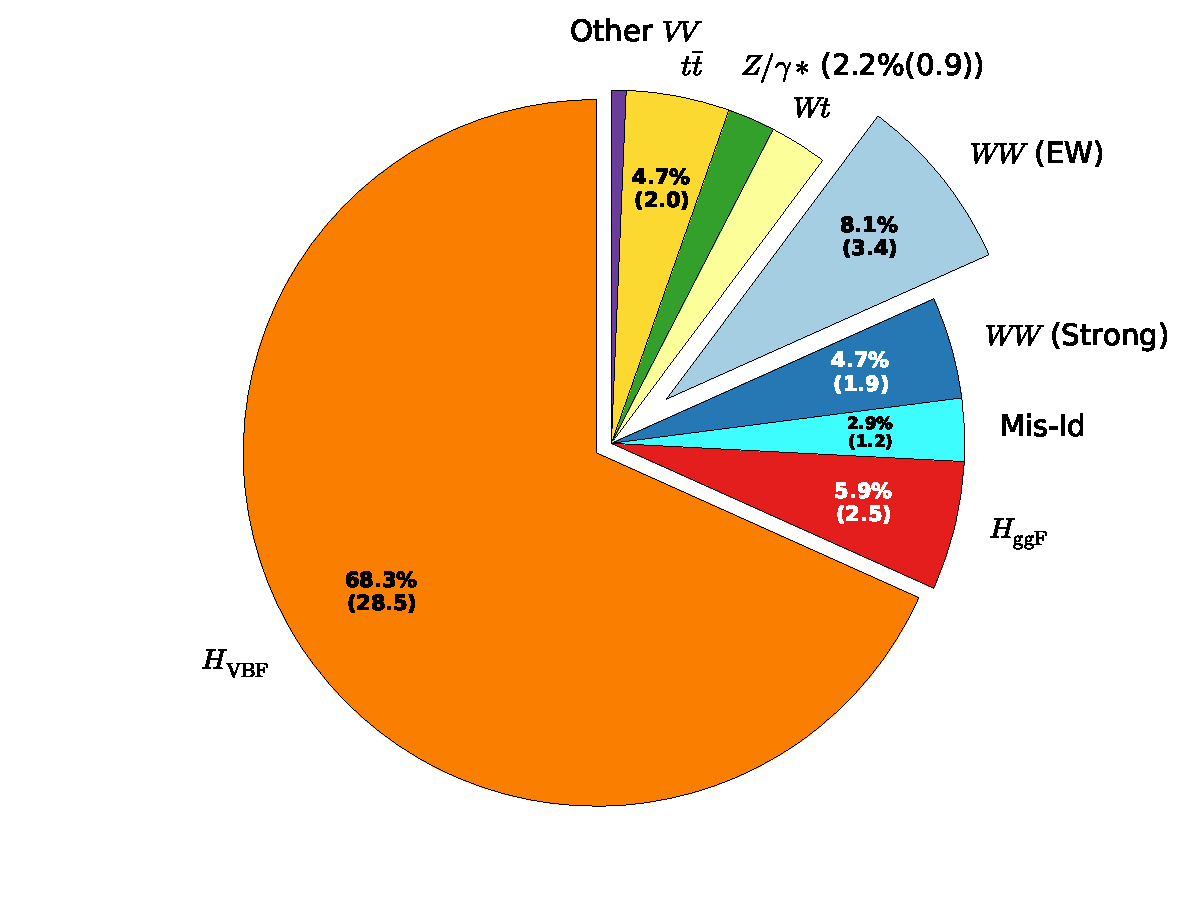
\includegraphics[width=0.49\textwidth,trim=35 0 0 0]{figures/plots/bkg-fraction-highest-bin/pie-chart-fractions-old.pdf}
        \label{fig:bkg-fractions-a}
    }
    \subfloat[Optimized EW $WW$ training fractions] {
        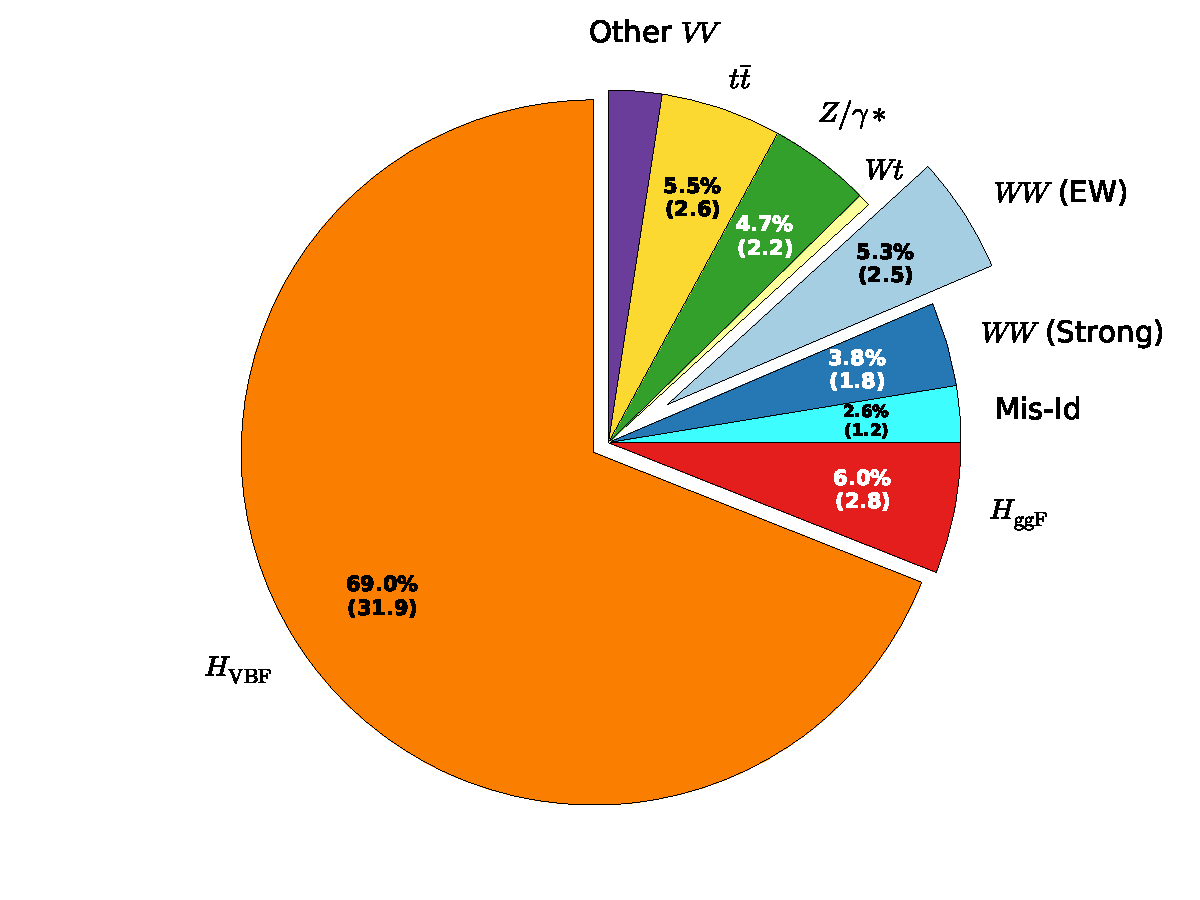
\includegraphics[width=0.49\textwidth,trim=35 0 0 0]{figures/plots/bkg-fraction-highest-bin/pie-chart-fractions-new.pdf}
        \label{fig:bkg-fractions-b}
    }
    \caption{Fraction of background in highest DNN output bin based on the validation set. }
    \label{fig:bkg-fractions}
\end{figure}

% Plots made with SFUsMLKit on cedar with:
% ./plot.py -c configs/HWW/winningSubmission.cfg --trainingFolderName dropout-02-5-fold-aggressive-lr-schedule-2-fine-scan-ewww-scan-etafix/210805_9_0.12_8226149877761426764
\begin{figure}[t]
    % \subfloat[] {
    %     \newImageResizeCustom{0.47}{figures/plots/sample-fractions/sig_vs_lrate.pdf}
    % }
    % \subfloat[] {
    \newImageResizeCustom{0.5}{figures/plots/sample-fractions/sig_vs_ew_fraction_lr9.pdf}
    % }
    \caption{}
    \label{fig:ew-fraction-scan}
\end{figure}



\FloatBarrier
\section{Distributions of the input variables in bins of the VBF DNN}
\label{app:dnn:input-vars}

\Cref{fig:dnn-inputs-vbf-top1,fig:dnn-inputs-vbf-top2,fig:dnn-inputs-vbf-top3,fig:dnn-inputs-hwwdecay,fig:dnn-inputs-top-sup} show distributions of the DNN input variables with different selections on the DNN output. This shows the effect of the DNN on the variables. 

\captionsetup[subfloat]{captionskip=5pt} % space between subfloat caption and image
\begin{figure}[ht]
    \centering
    \subfloat[$\mjj$]{
        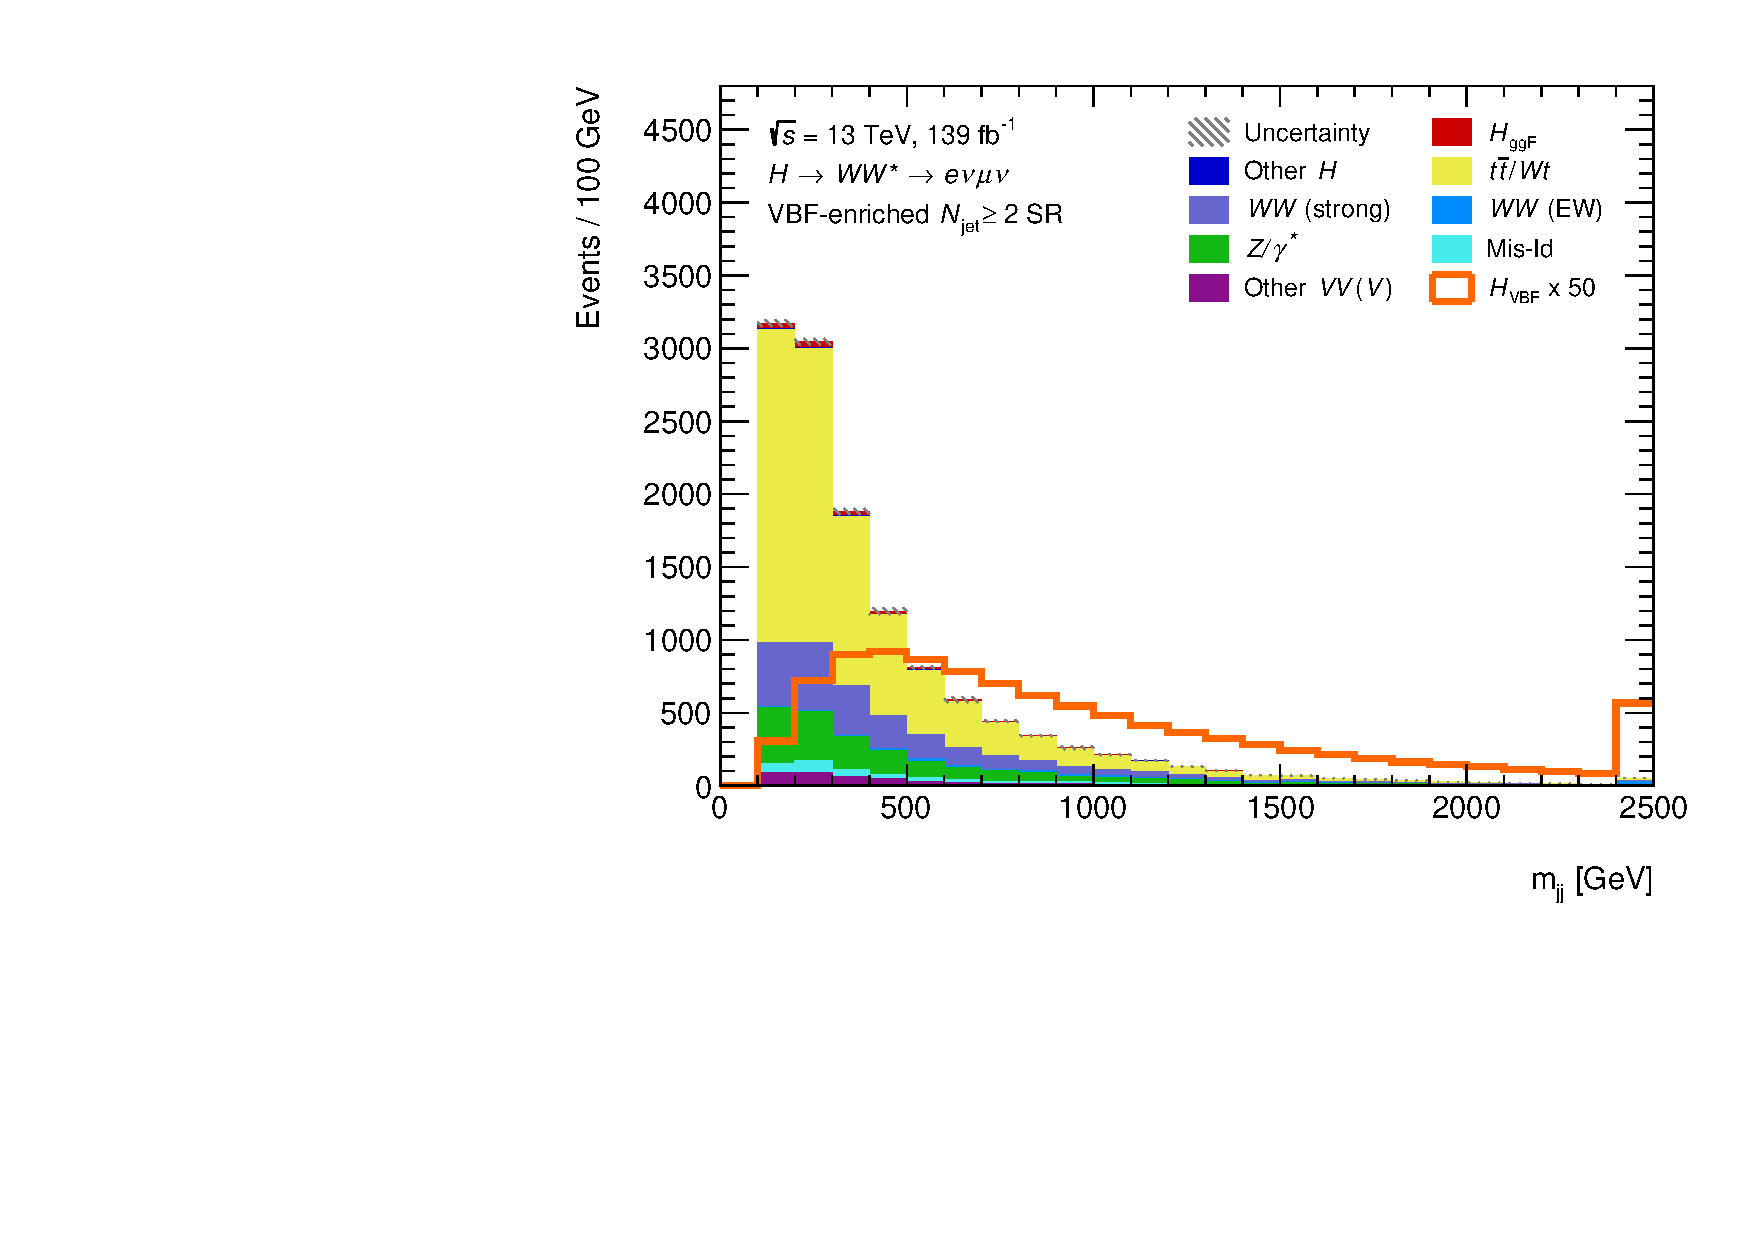
\includegraphics[width=0.32\textwidth]{figures/hww/dnn/blinded/run2-emme-CutVBF_SR-Mjj-lin.pdf} \hfill
        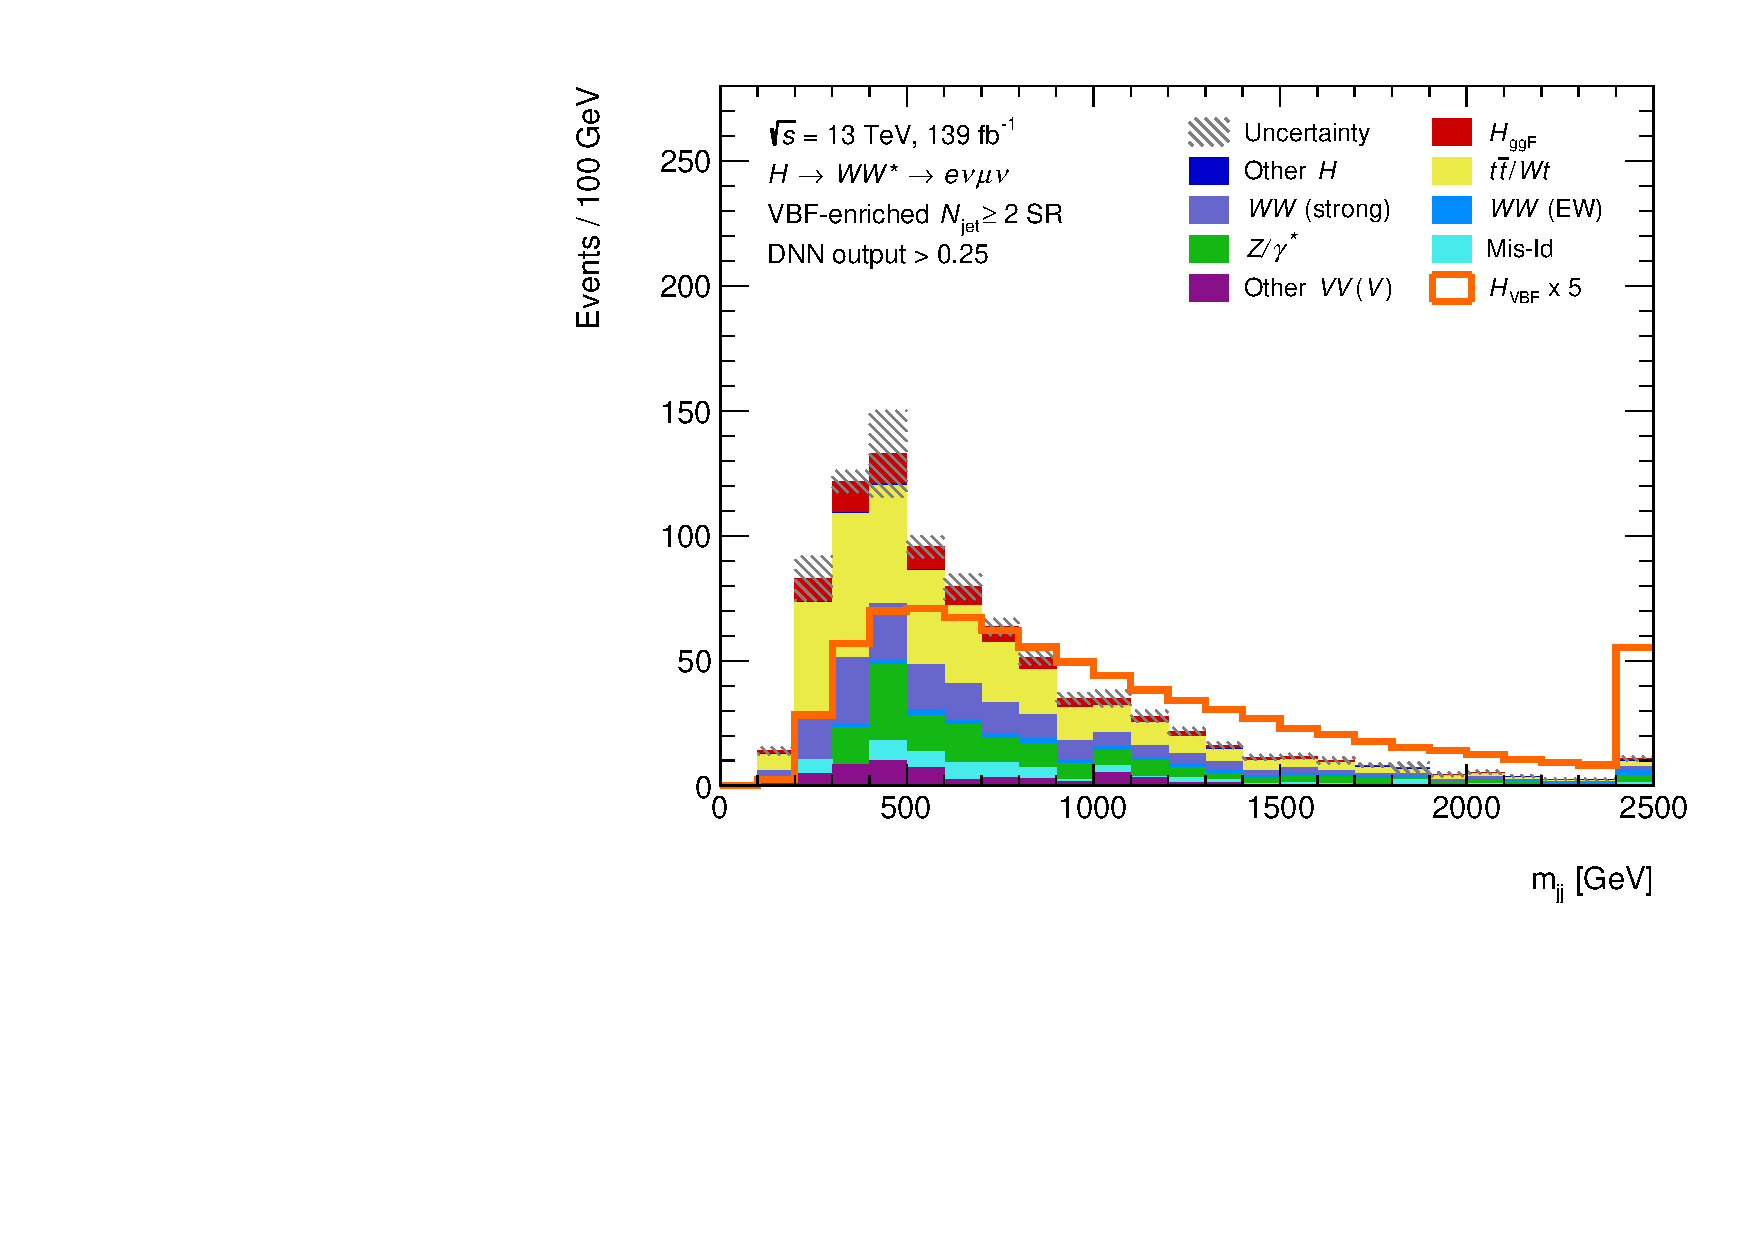
\includegraphics[width=0.32\textwidth]{figures/hww/dnn/blinded/run2-emme-CutVBFSR_DNN25-Mjj-lin.pdf} \hfill
        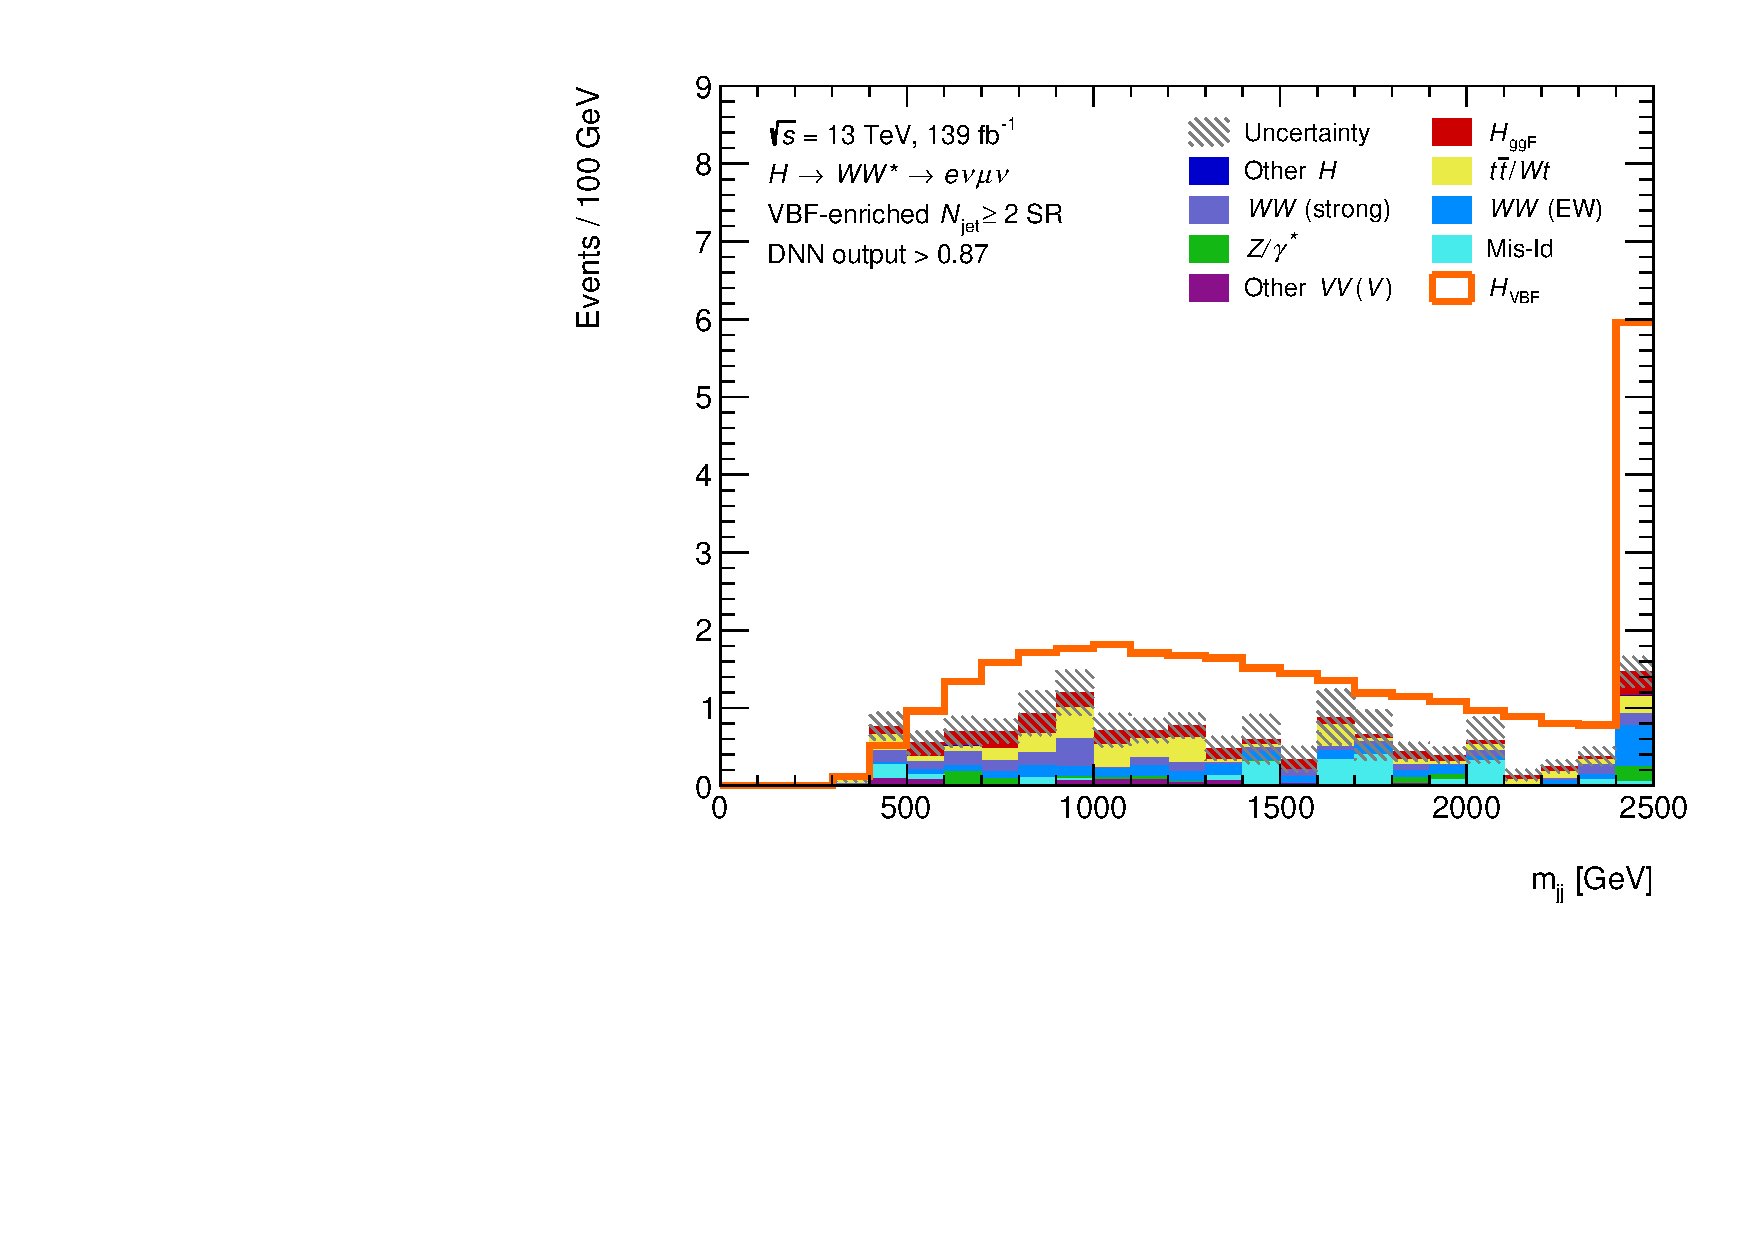
\includegraphics[width=0.32\textwidth]{figures/hww/dnn/blinded/run2-emme-CutVBFSR_DNN87-Mjj-lin.pdf}
    } \\
    \subfloat[$\dyjj$]{
        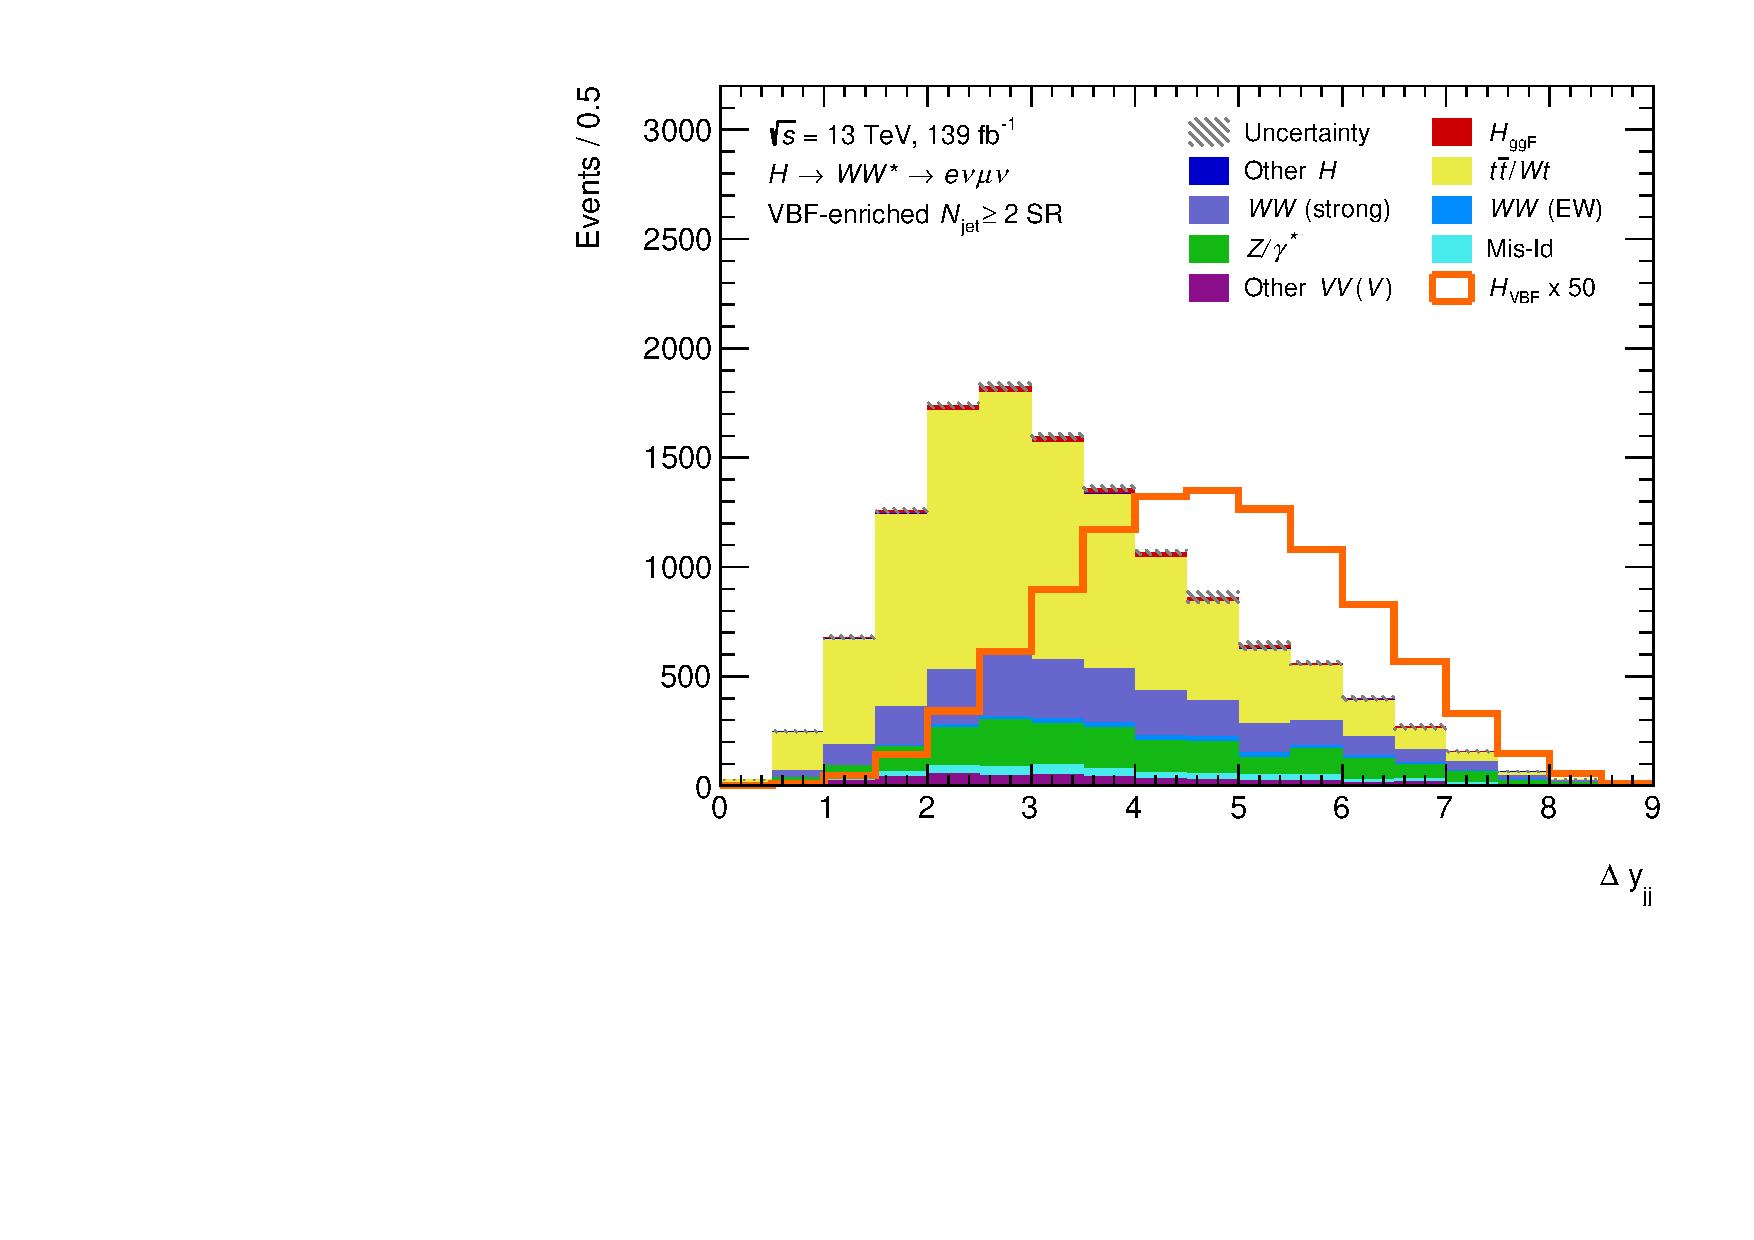
\includegraphics[width=0.32\textwidth]{figures/hww/dnn/blinded/run2-emme-CutVBF_SR-DYjj-lin.pdf} \hfill
        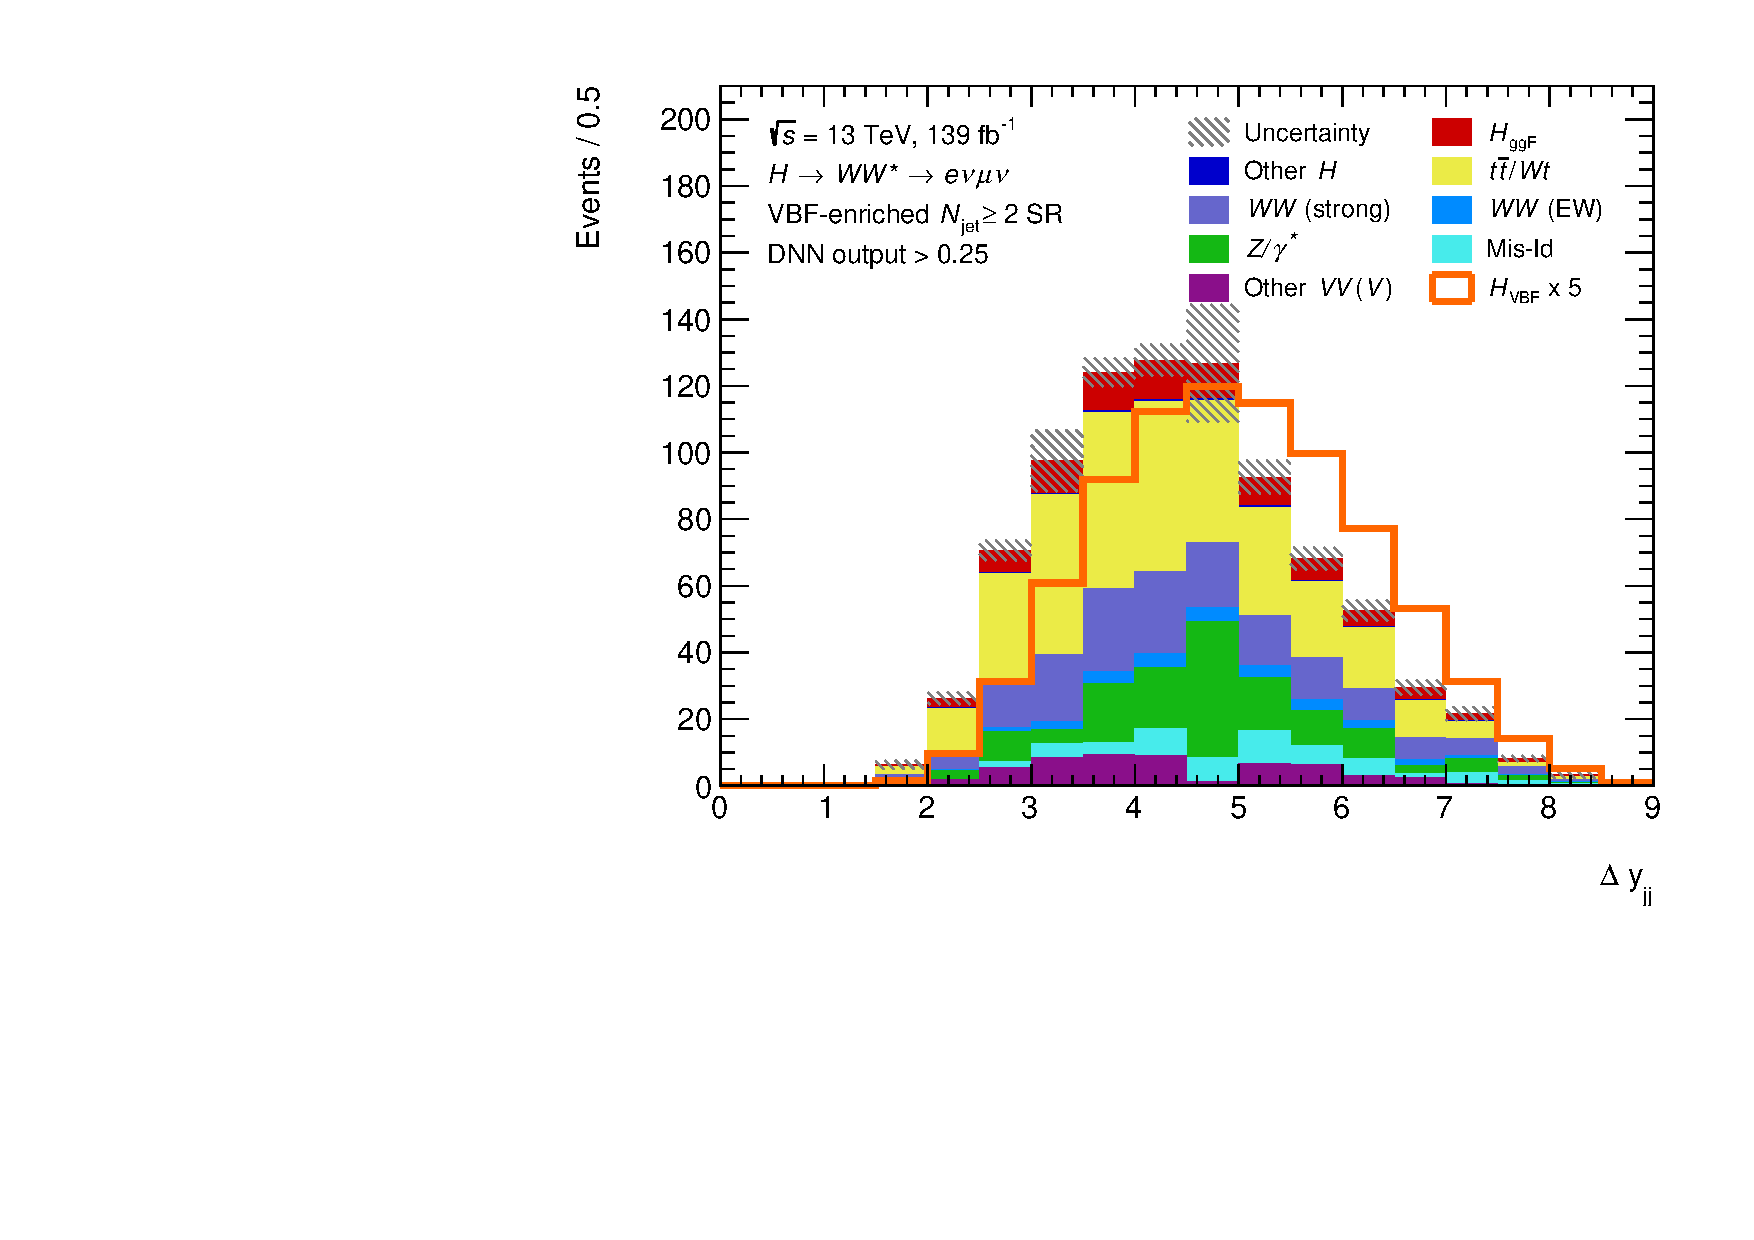
\includegraphics[width=0.32\textwidth]{figures/hww/dnn/blinded/run2-emme-CutVBFSR_DNN25-DYjj-lin.pdf} \hfill
        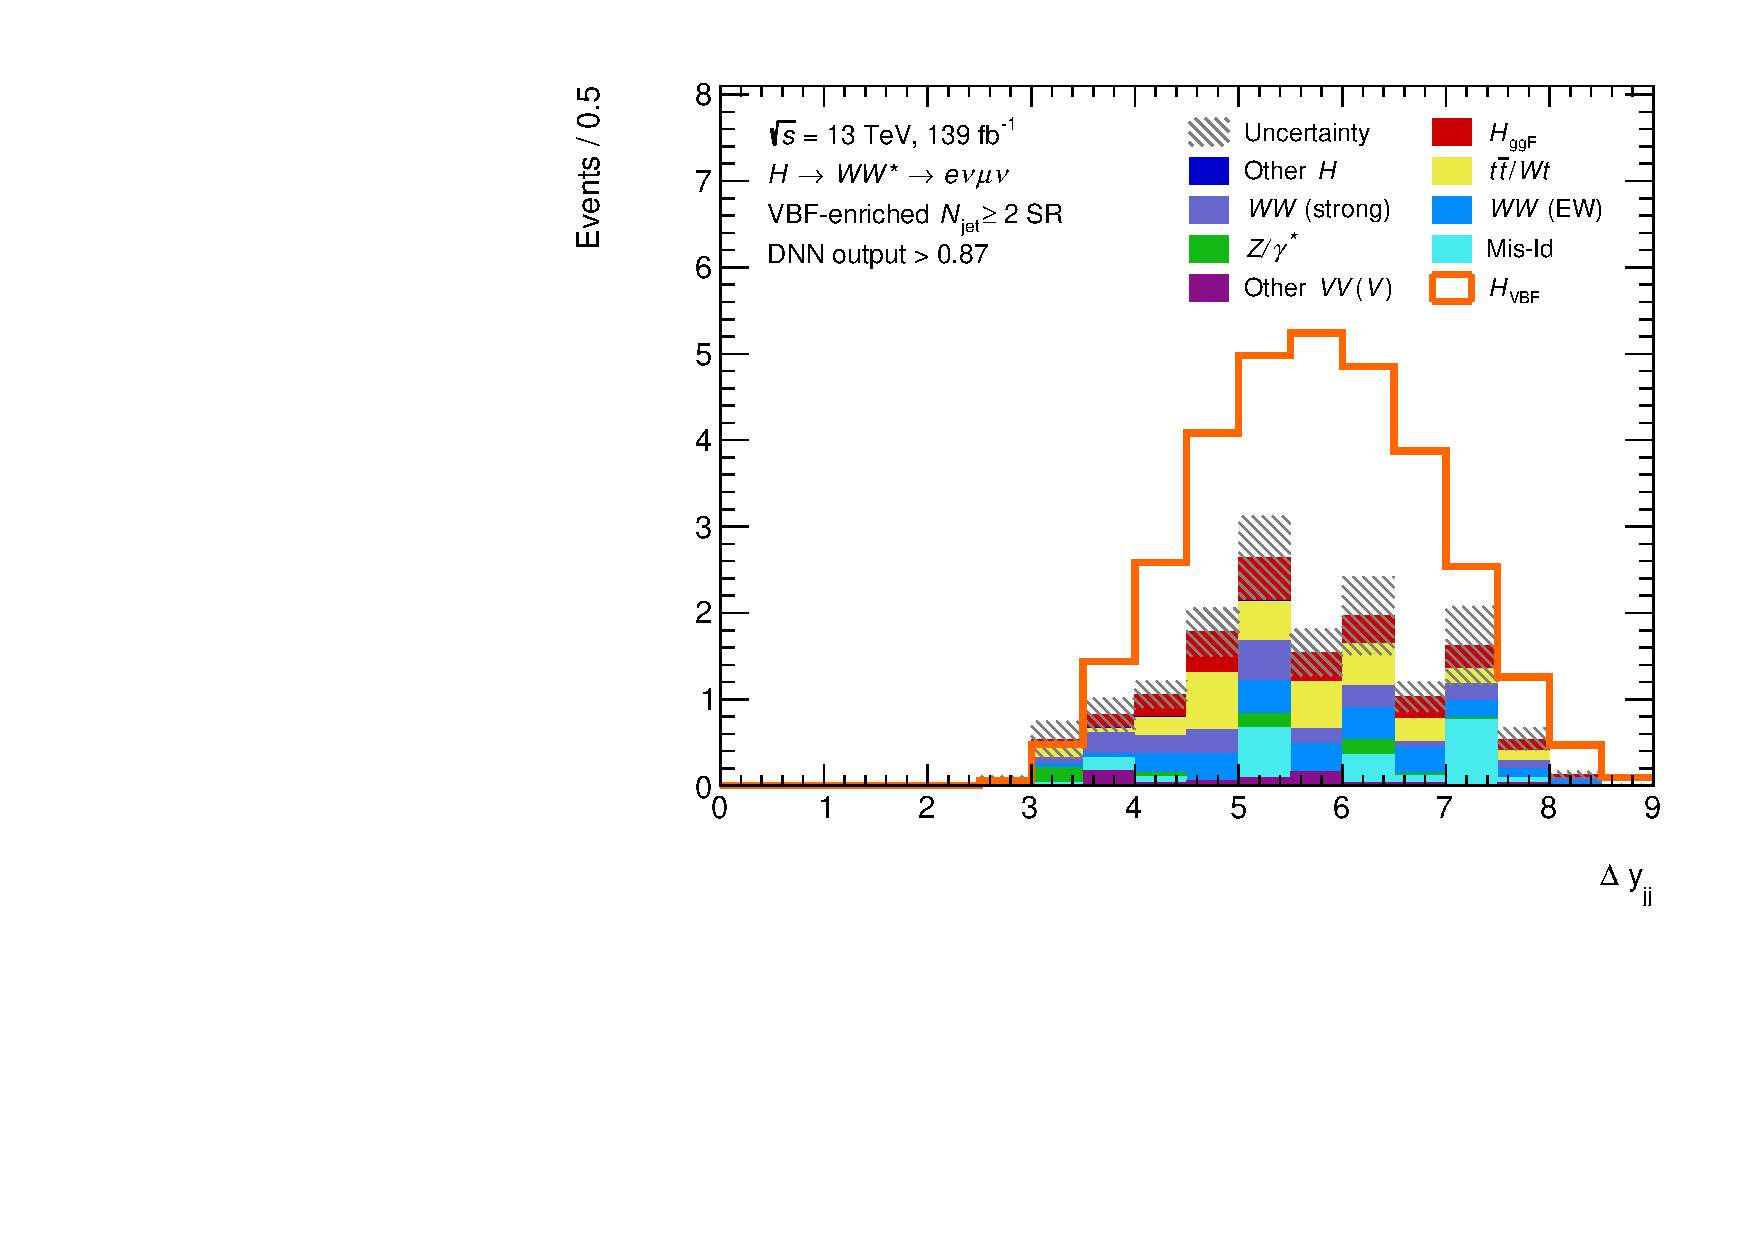
\includegraphics[width=0.32\textwidth]{figures/hww/dnn/blinded/run2-emme-CutVBFSR_DNN87-DYjj-lin.pdf}
    } \\
    \subfloat[$\lepetacent$]{
        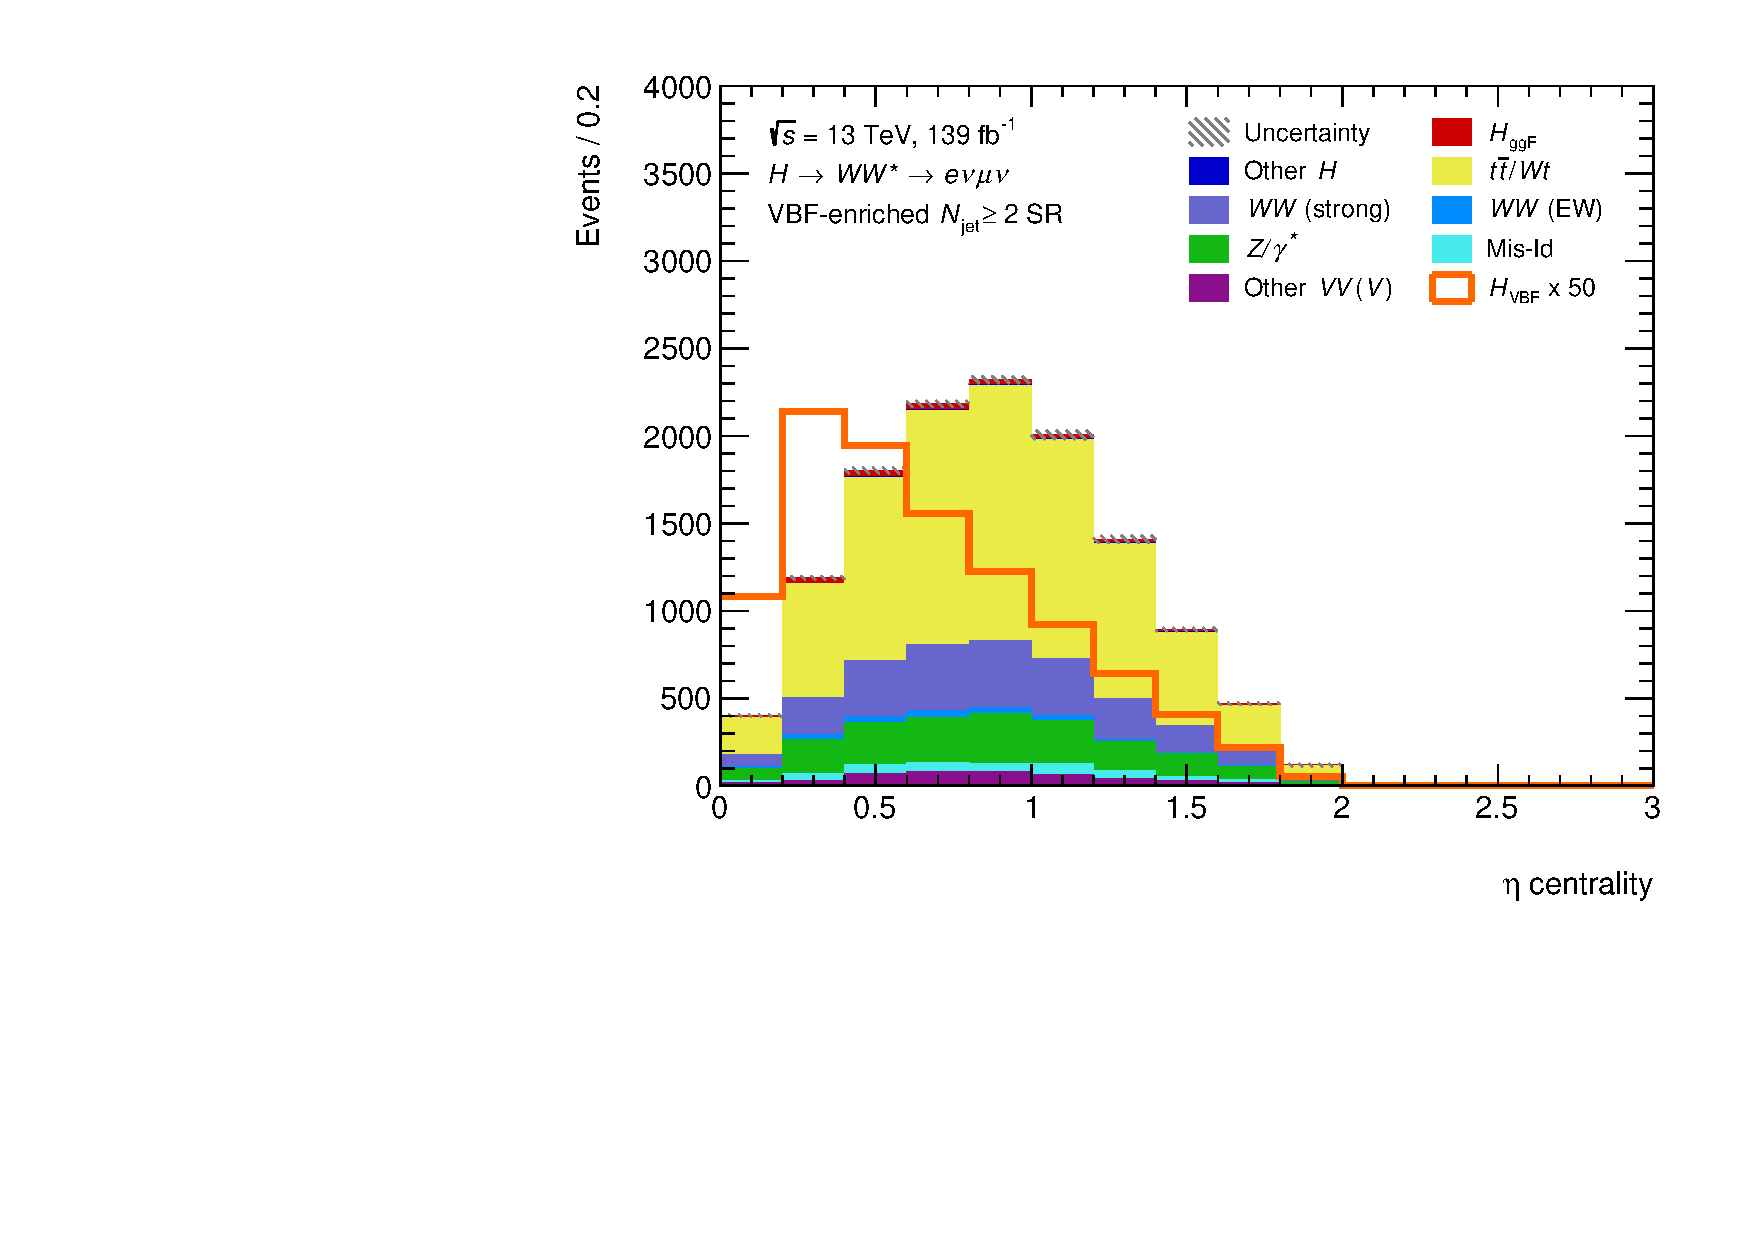
\includegraphics[width=0.32\textwidth]{figures/hww/dnn/blinded/run2-emme-CutVBF_SR-contOLV-lin.pdf} \hfill
        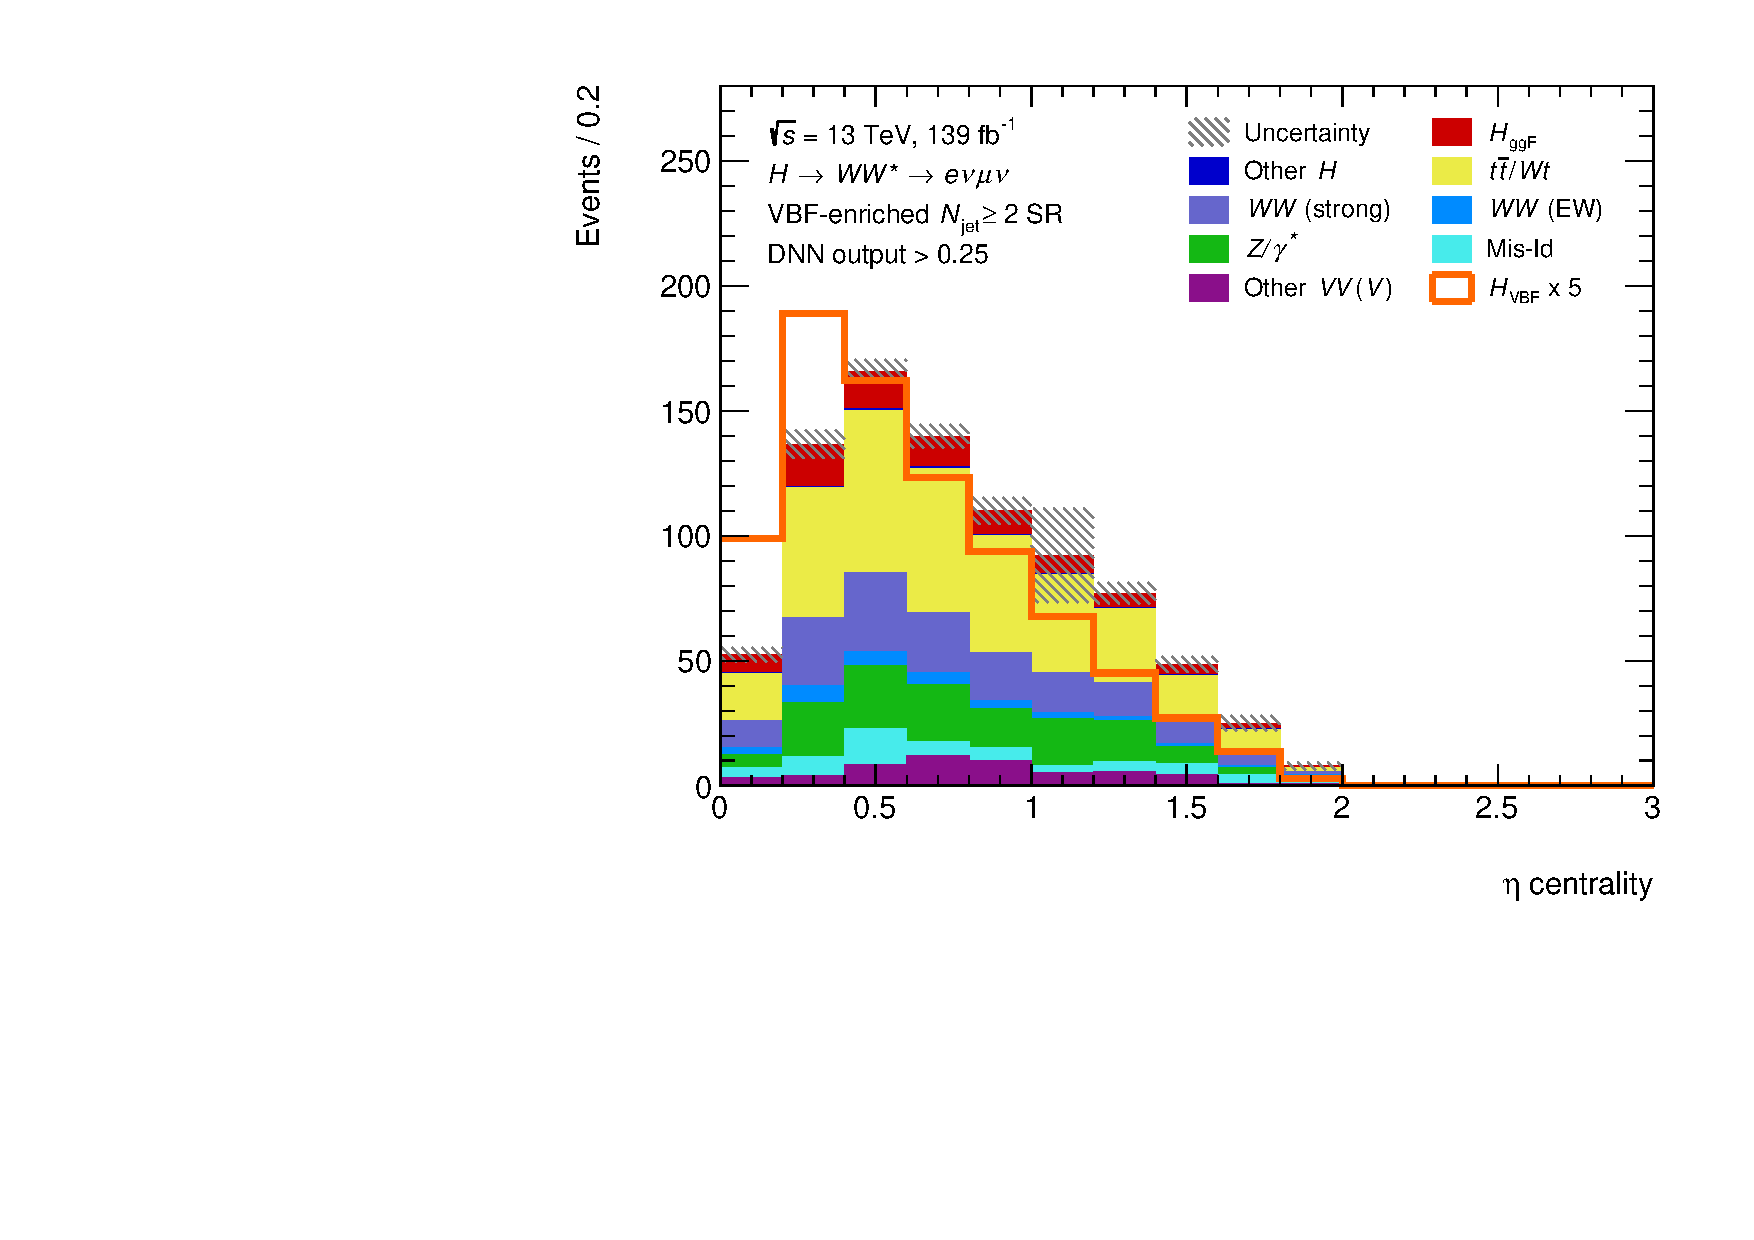
\includegraphics[width=0.32\textwidth]{figures/hww/dnn/blinded/run2-emme-CutVBFSR_DNN25-contOLV-lin.pdf} \hfill
        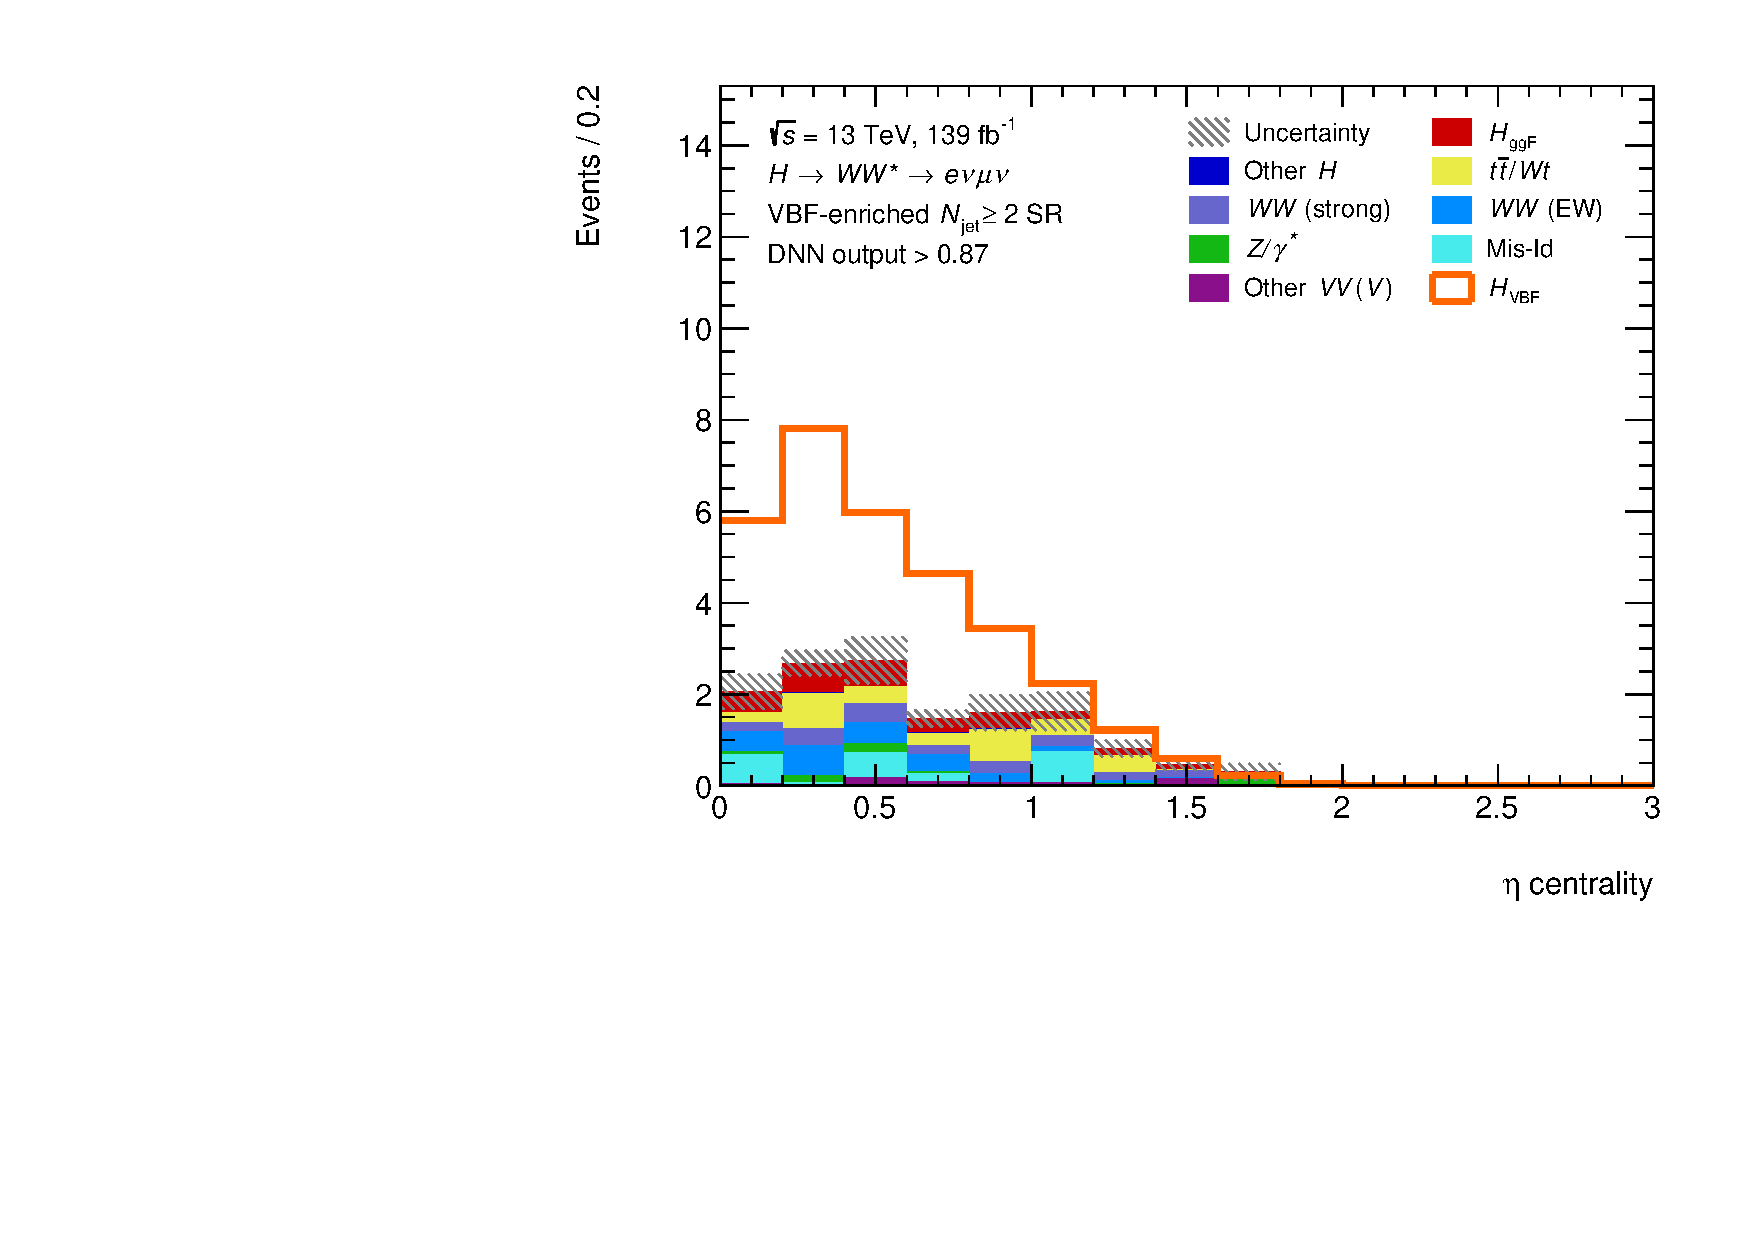
\includegraphics[width=0.32\textwidth]{figures/hww/dnn/blinded/run2-emme-CutVBFSR_DNN87-contOLV-lin.pdf}
    } \\
    {\caption{Distributions of $\dphill$, $\mll$, $\lepetacent$ in the VBF signal region.
        Each row corresponds to one variable with different selections made on the DNN output.
        \label{fig:dnn-inputs-vbf-top1} }}
\end{figure}


\begin{figure}[h]
    \centering
    \subfloat[$\mlonejtwo$]{
        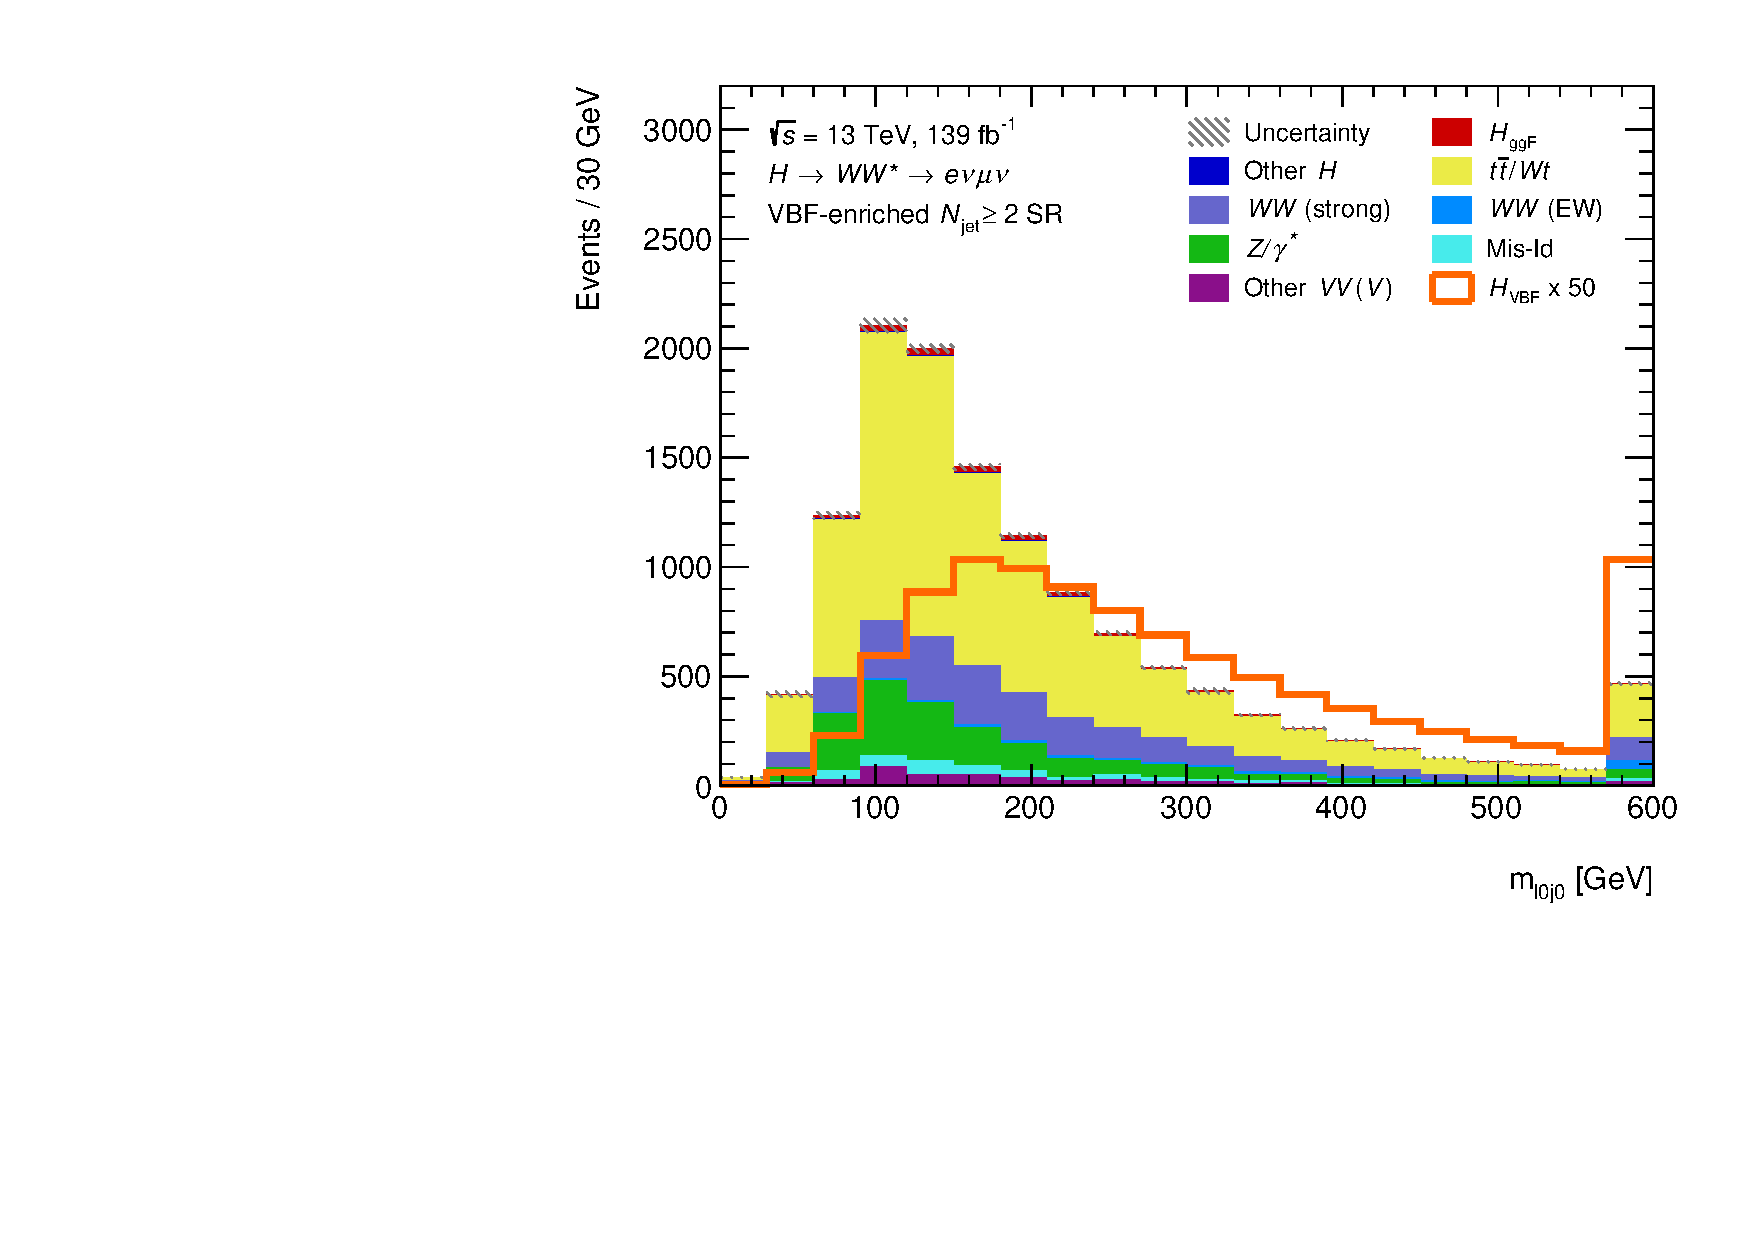
\includegraphics[width=0.32\textwidth]{figures/hww/dnn/blinded/run2-emme-CutVBF_SR-Ml0j0-lin.pdf} \hfill
        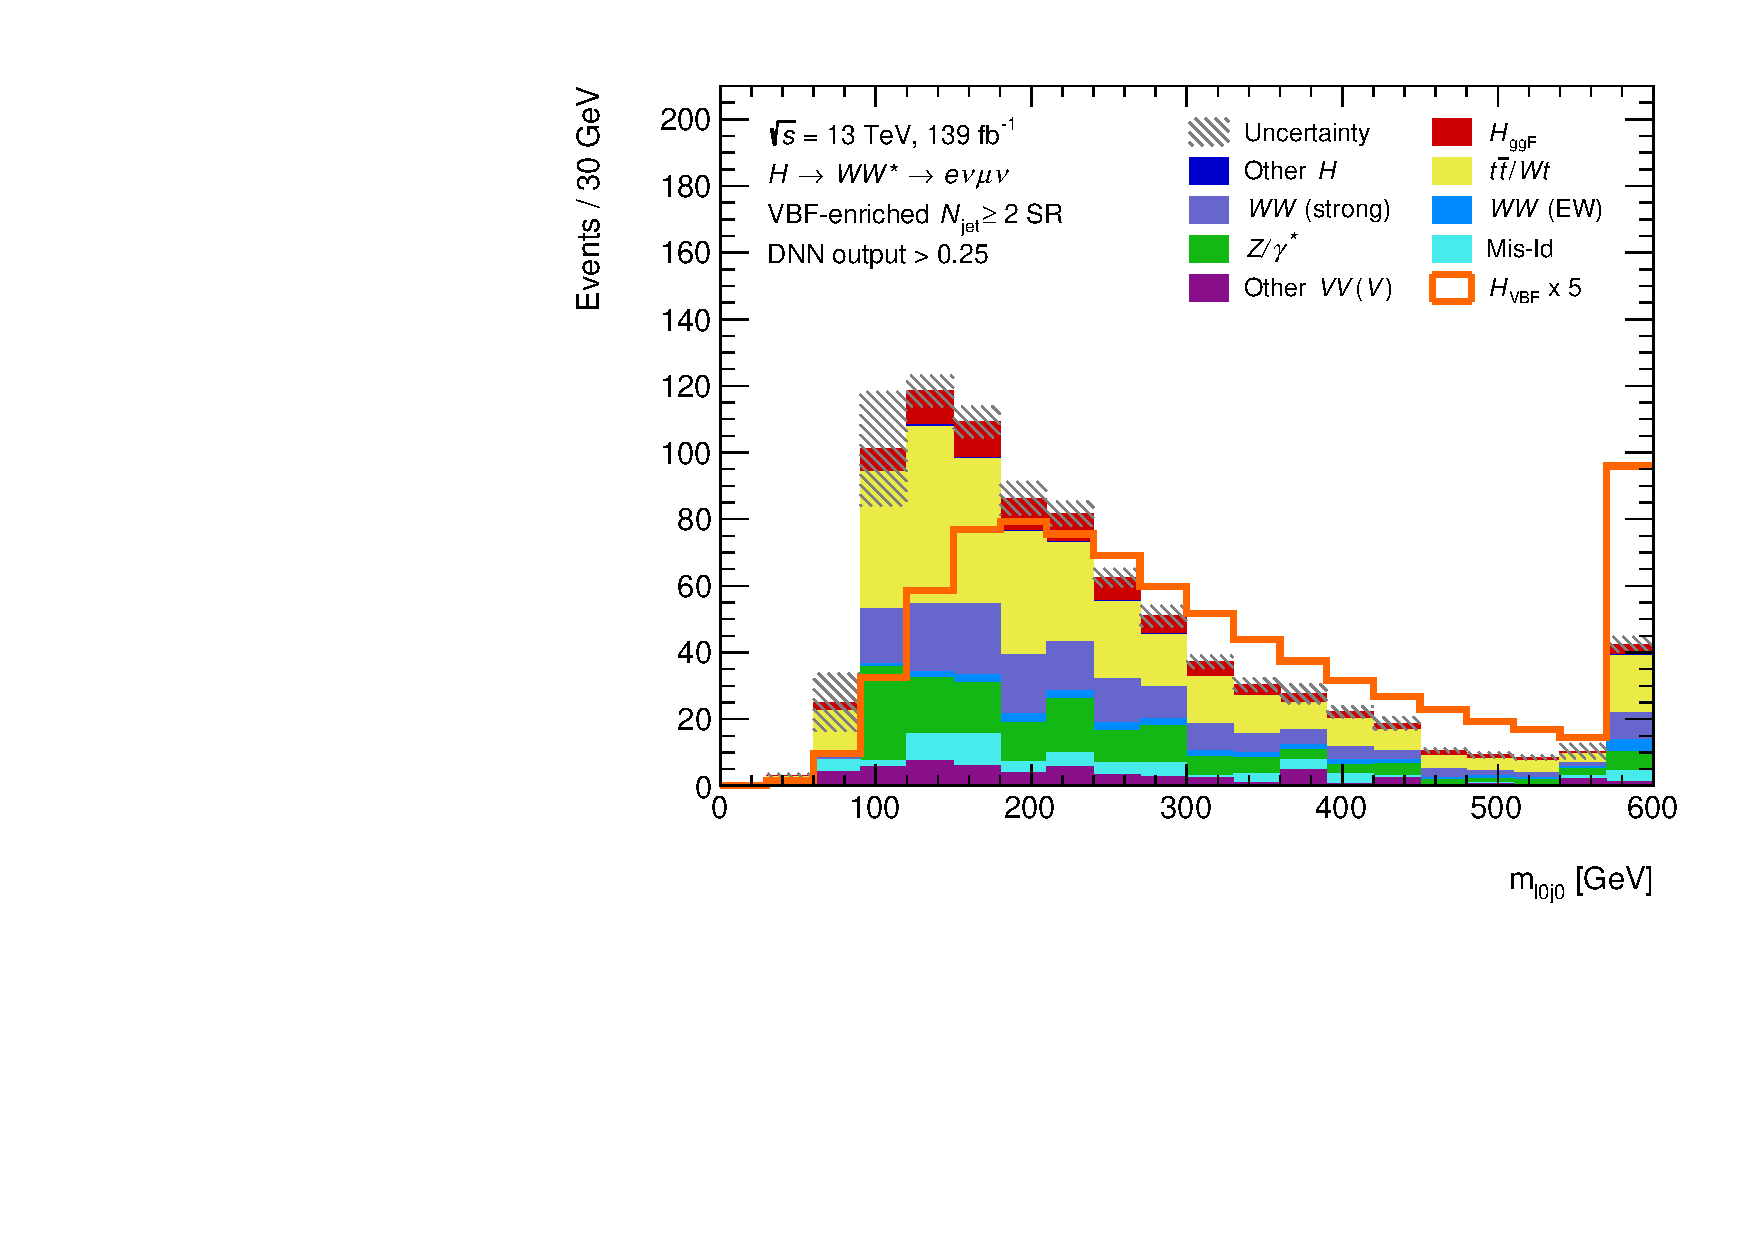
\includegraphics[width=0.32\textwidth]{figures/hww/dnn/blinded/run2-emme-CutVBFSR_DNN25-Ml0j0-lin.pdf} \hfill
        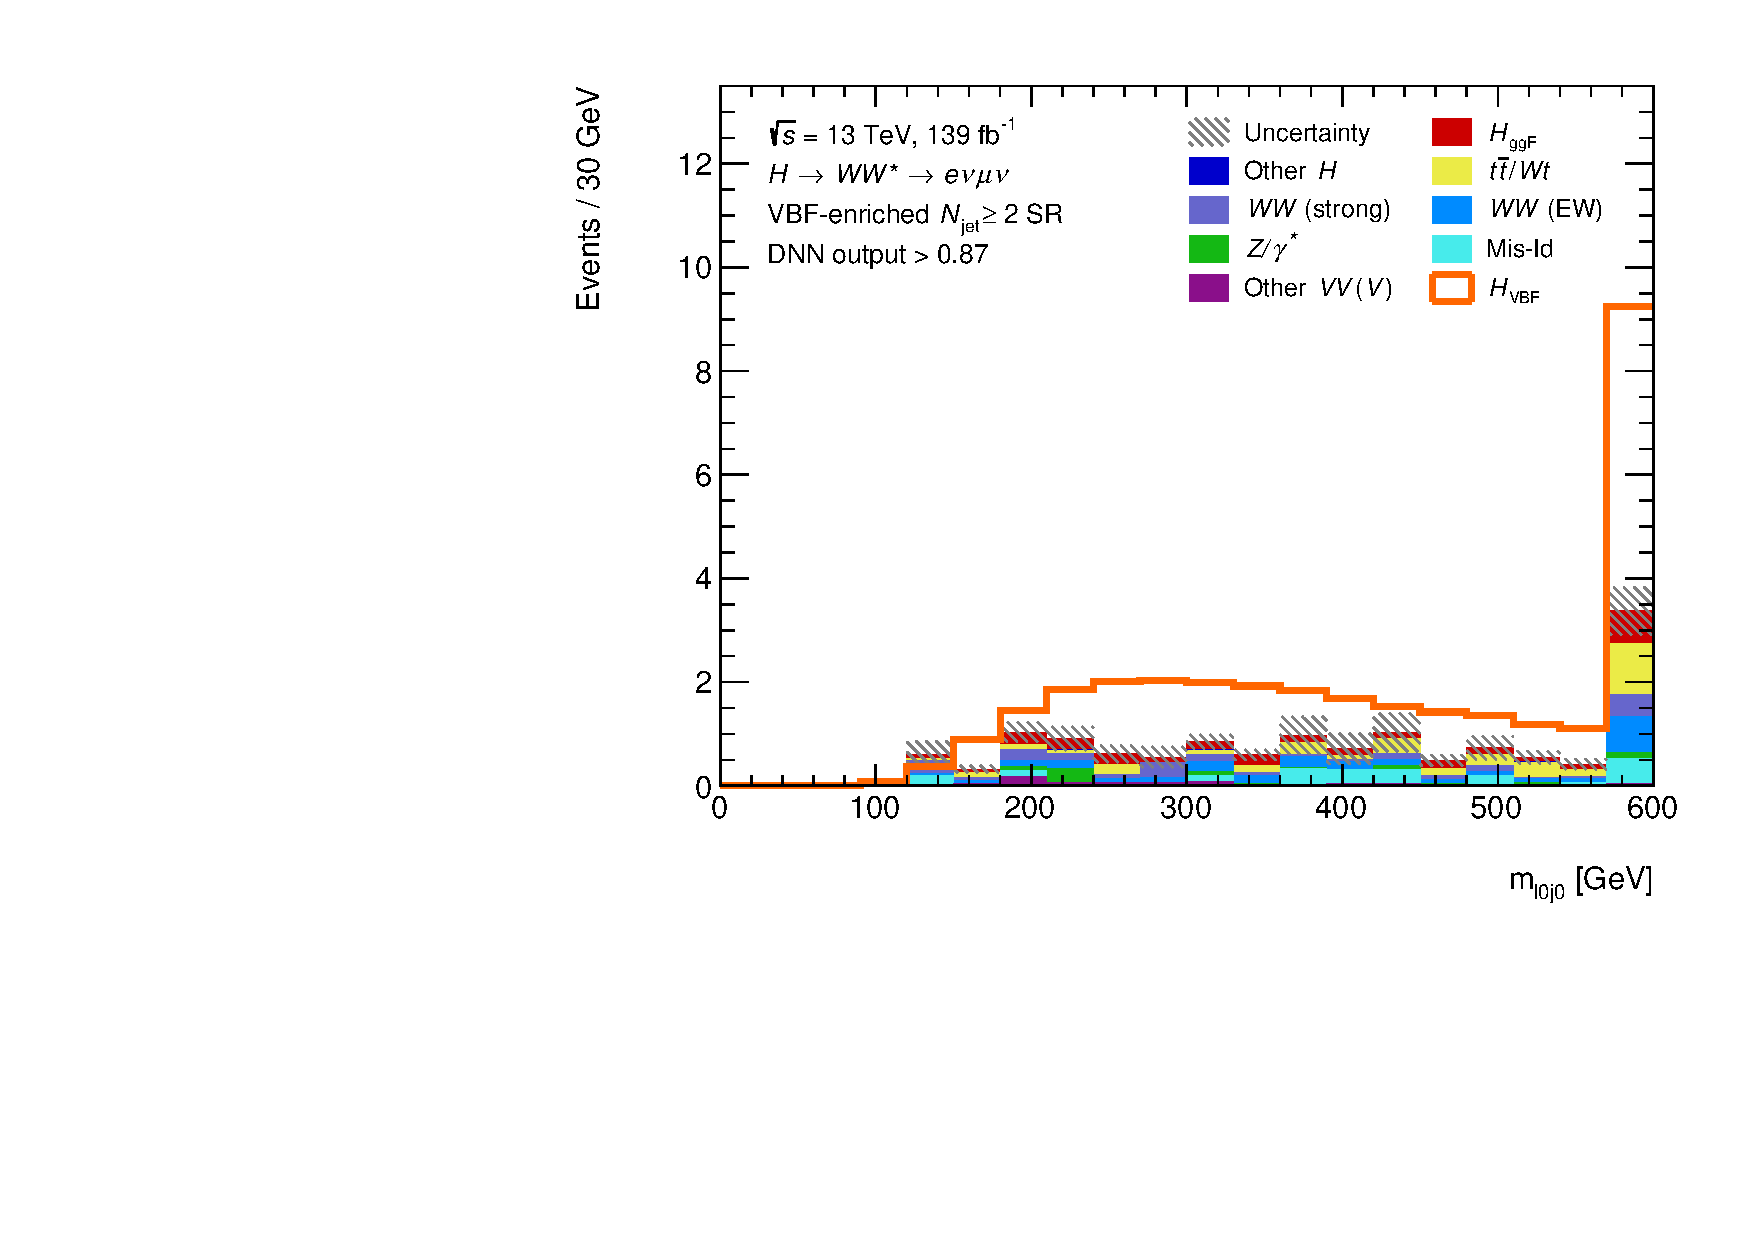
\includegraphics[width=0.32\textwidth]{figures/hww/dnn/blinded/run2-emme-CutVBFSR_DNN87-Ml0j0-lin.pdf}
    } \\
    \subfloat[$\mltwojone$]{
        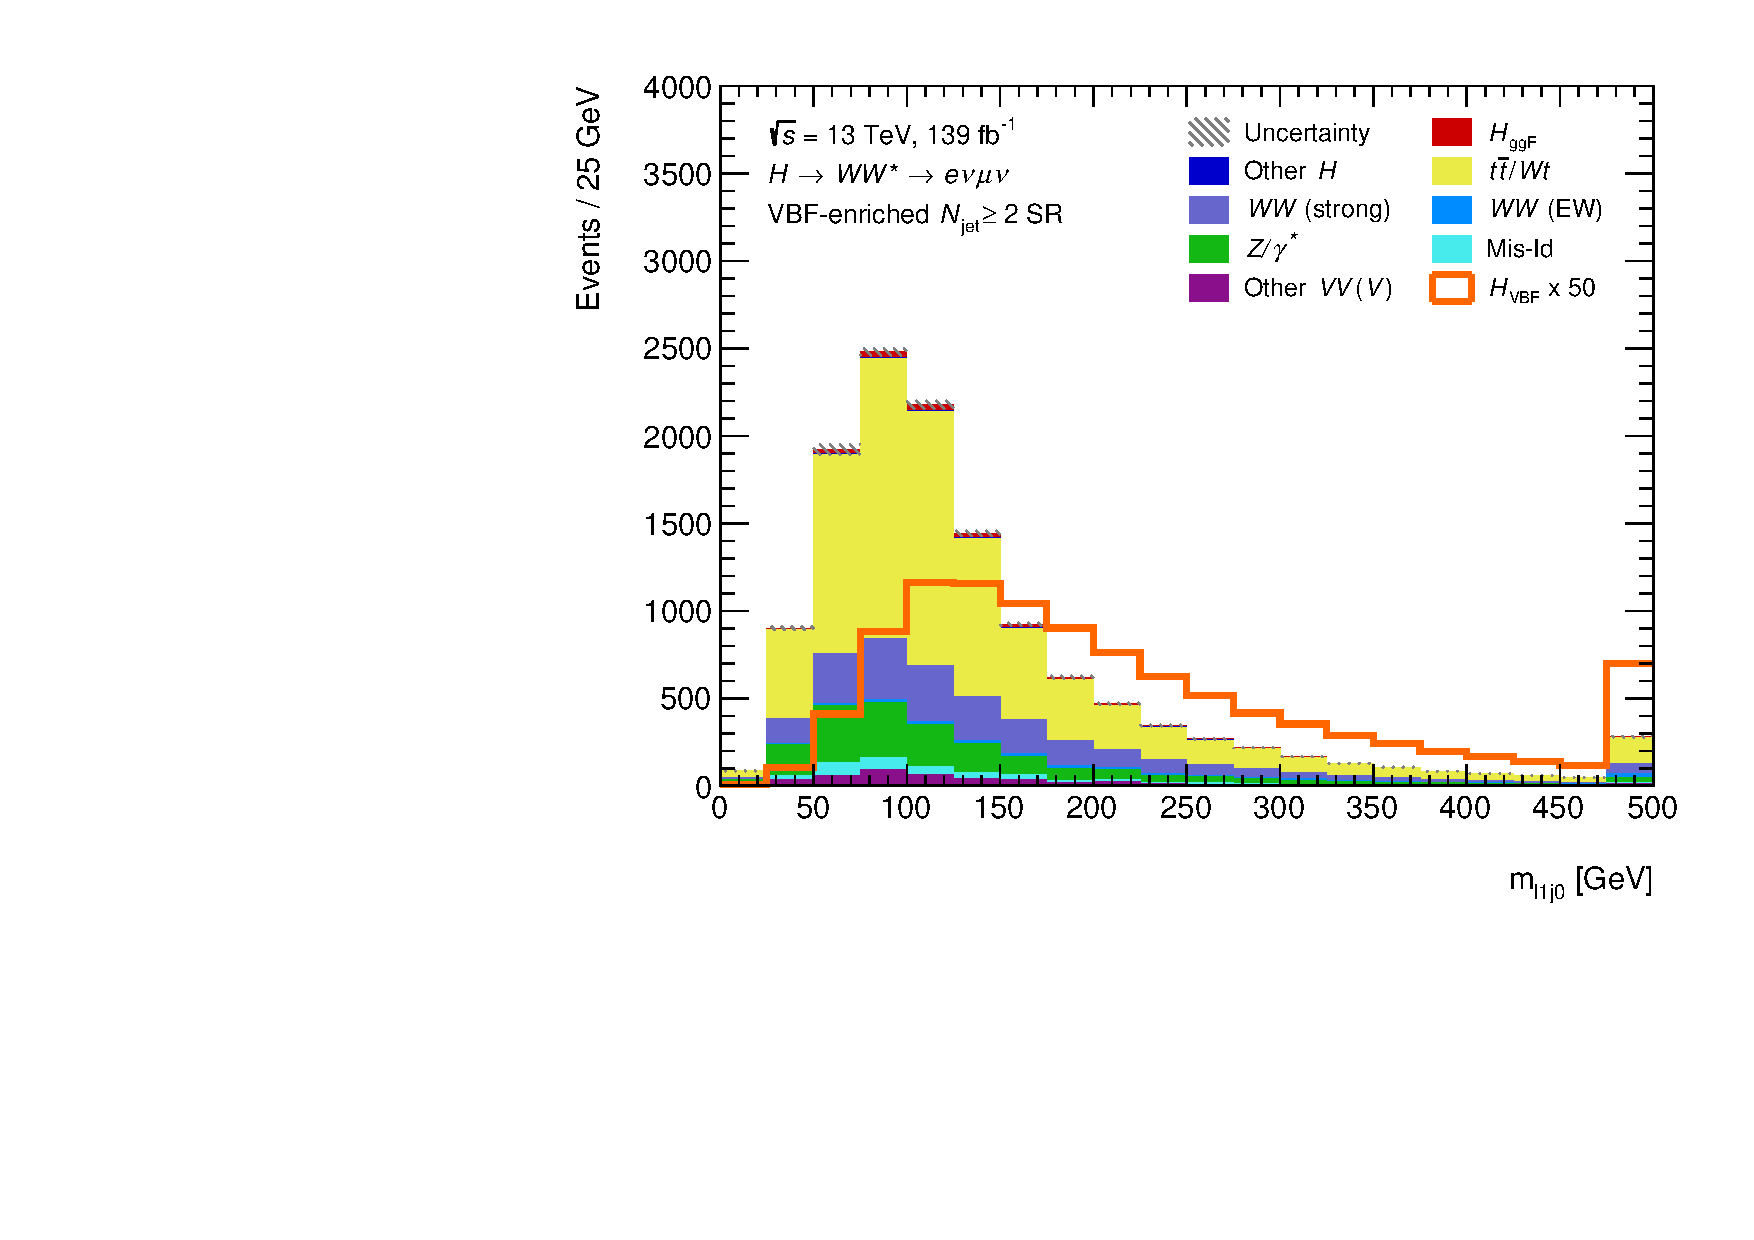
\includegraphics[width=0.32\textwidth]{figures/hww/dnn/blinded/run2-emme-CutVBF_SR-Ml1j0-lin.pdf} \hfill
        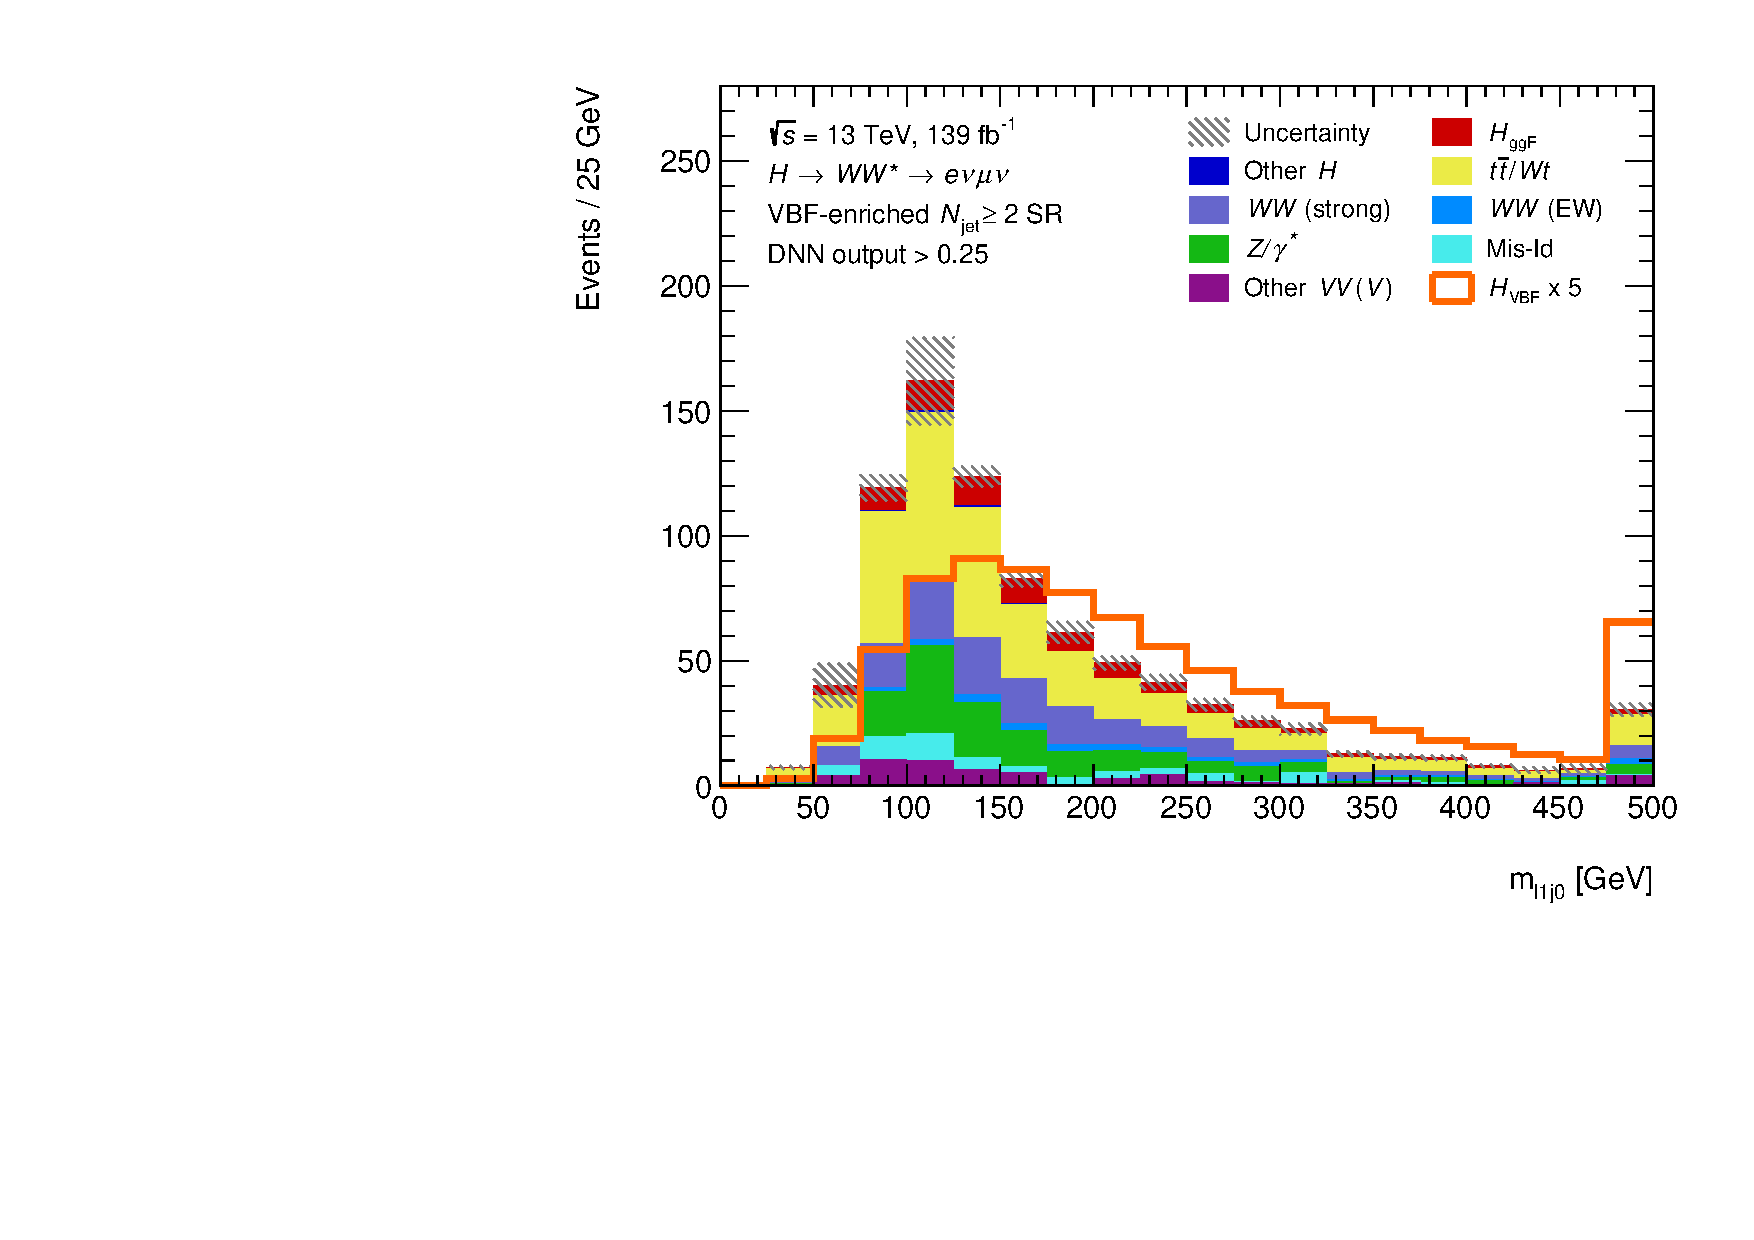
\includegraphics[width=0.32\textwidth]{figures/hww/dnn/blinded/run2-emme-CutVBFSR_DNN25-Ml1j0-lin.pdf} \hfill
        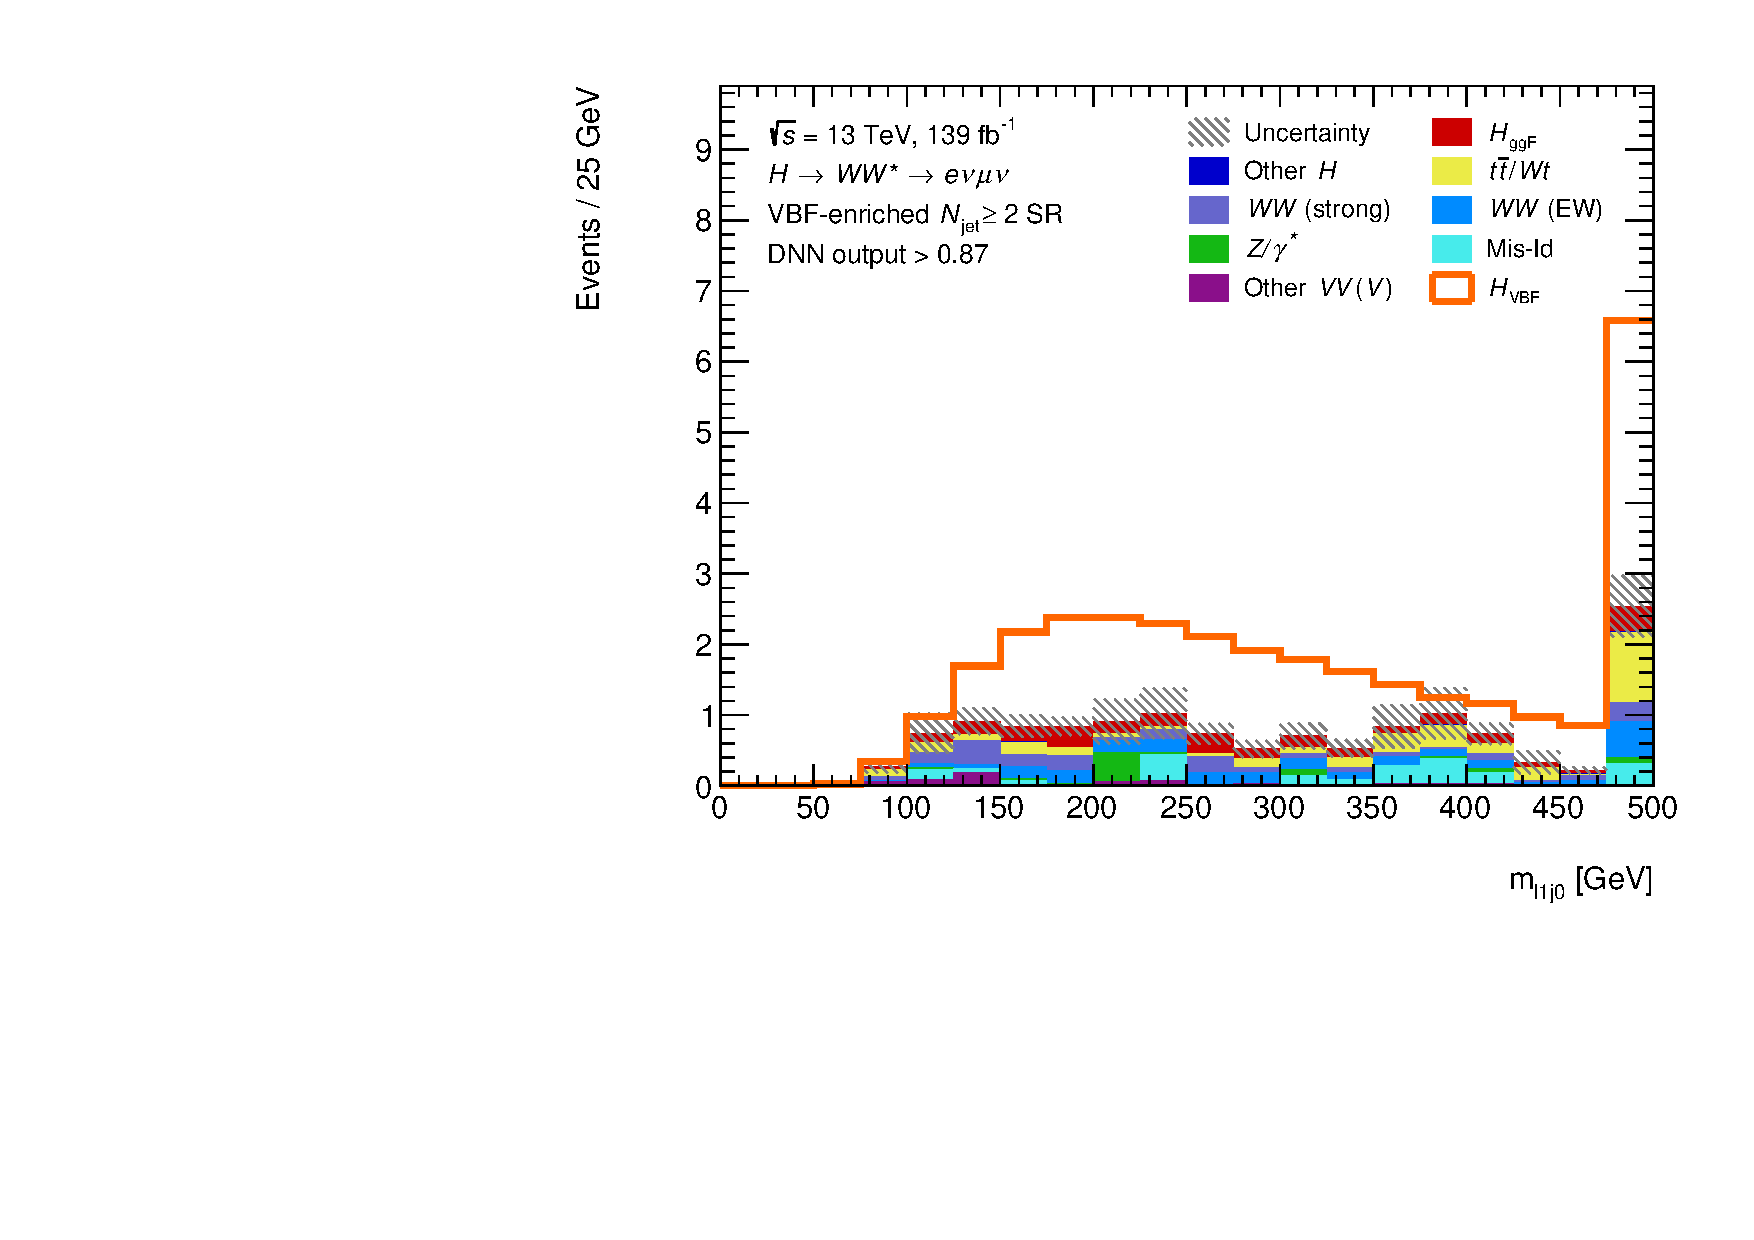
\includegraphics[width=0.32\textwidth]{figures/hww/dnn/blinded/run2-emme-CutVBFSR_DNN87-Ml1j0-lin.pdf}
    } \\
    \subfloat[$\mlonejtwo$]{
        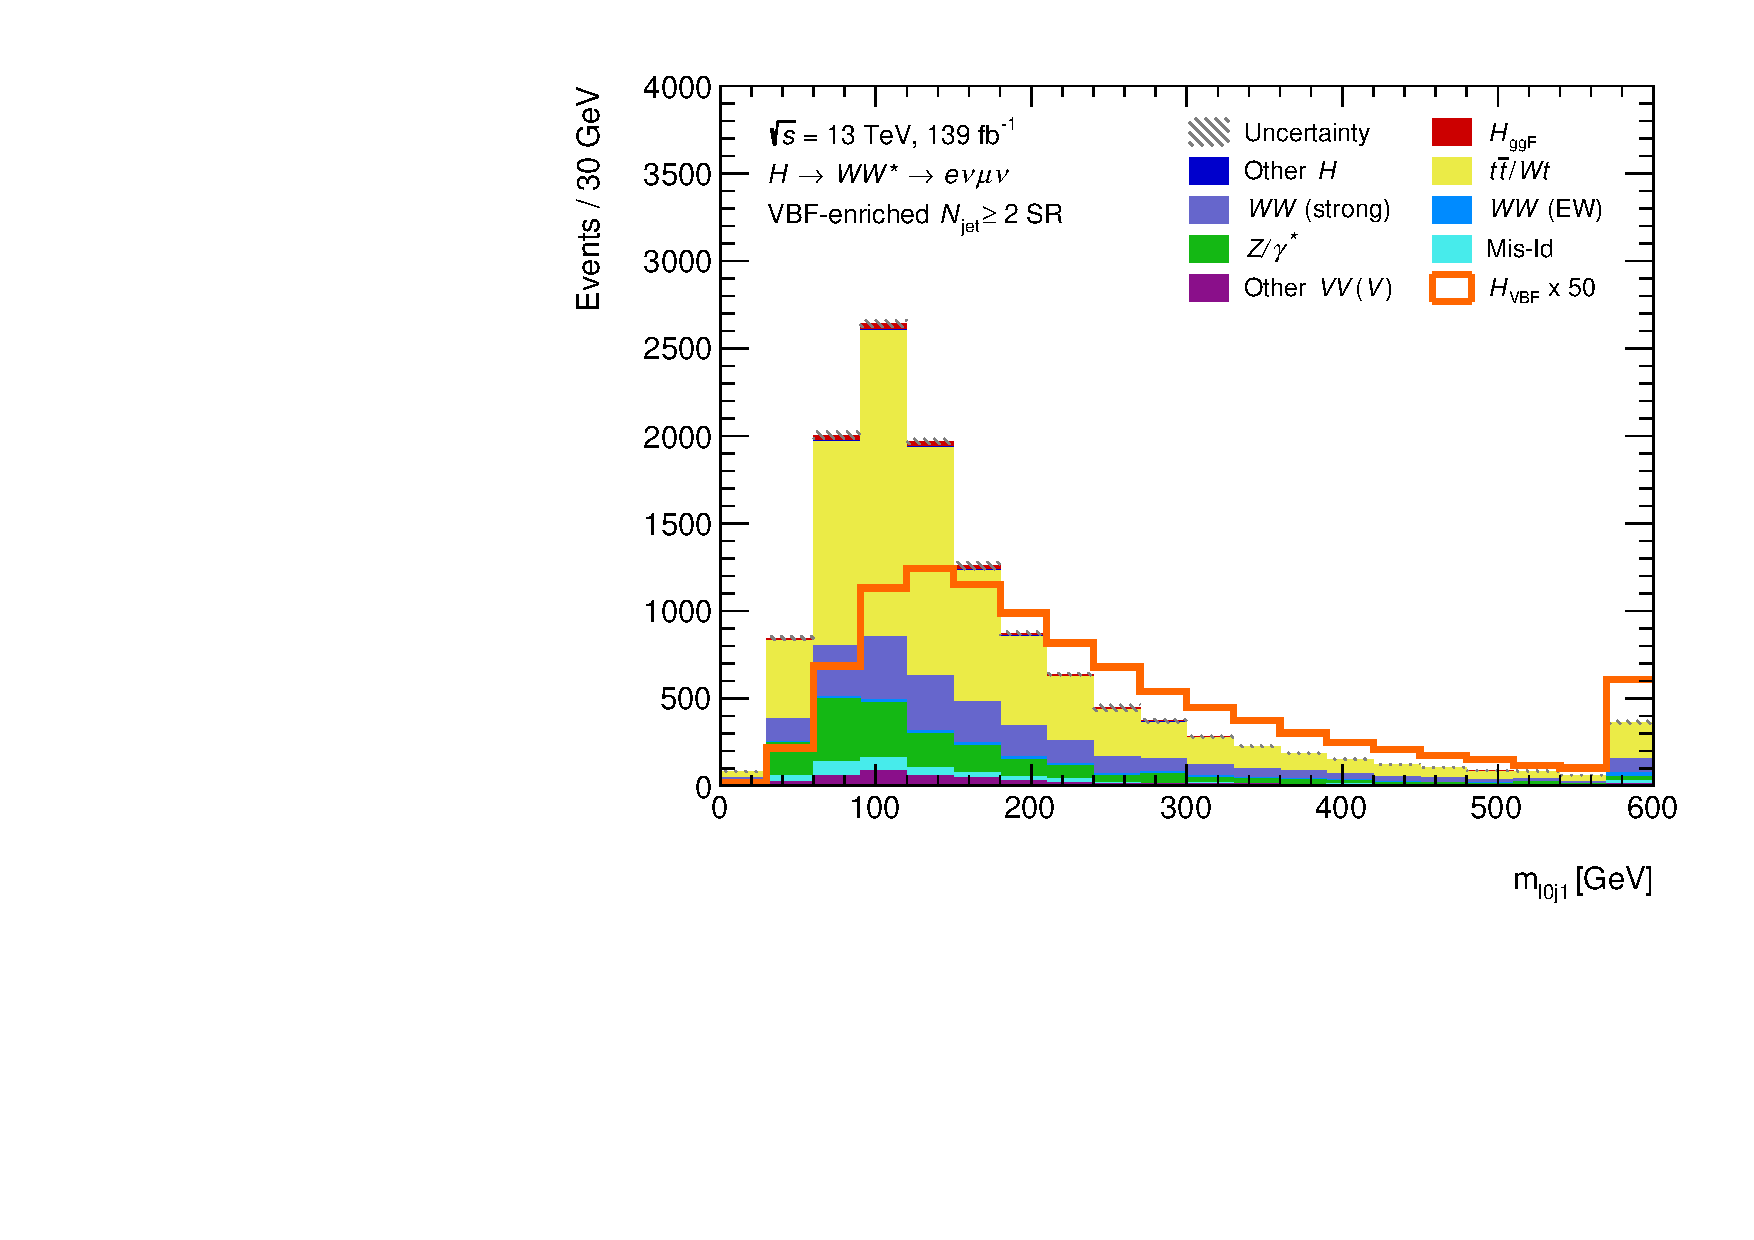
\includegraphics[width=0.32\textwidth]{figures/hww/dnn/blinded/run2-emme-CutVBF_SR-Ml0j1-lin.pdf} \hfill
        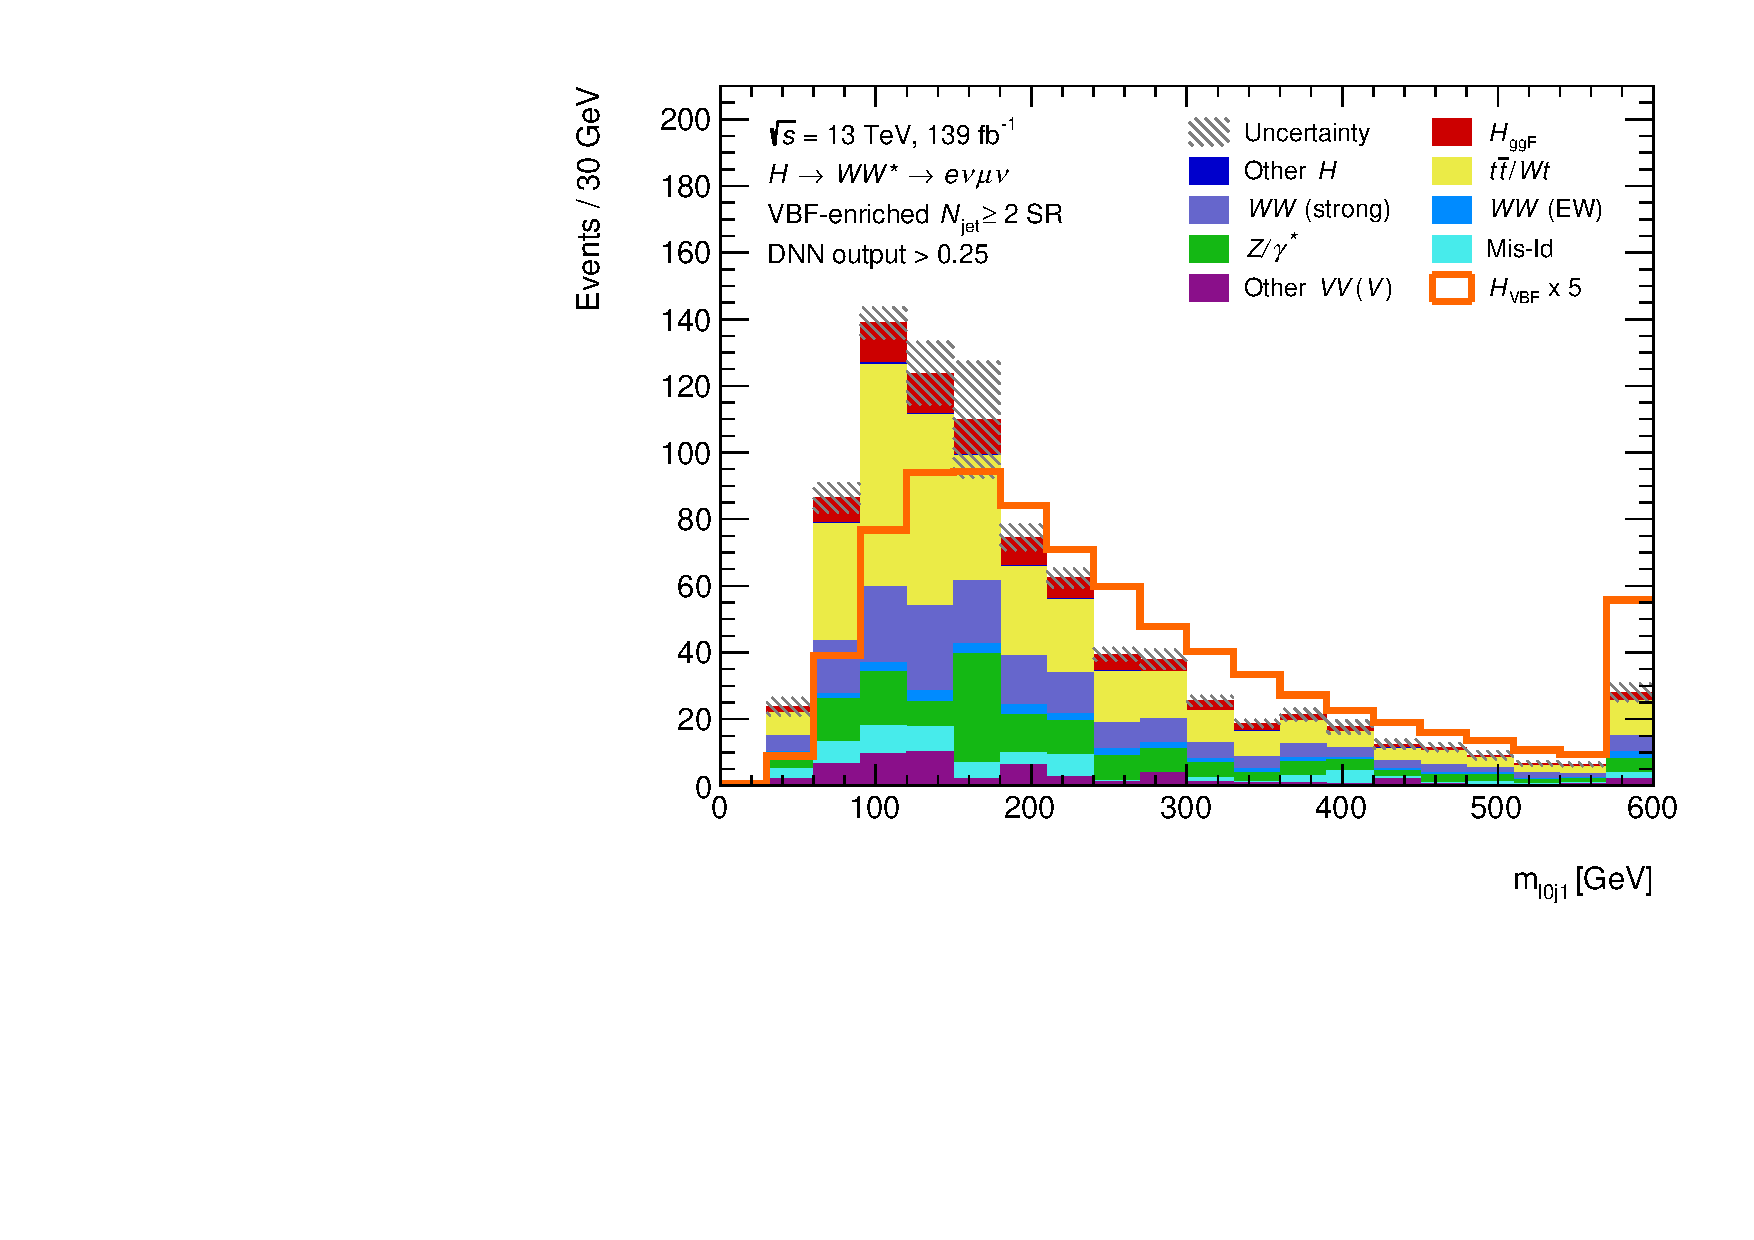
\includegraphics[width=0.32\textwidth]{figures/hww/dnn/blinded/run2-emme-CutVBFSR_DNN25-Ml0j1-lin.pdf} \hfill
        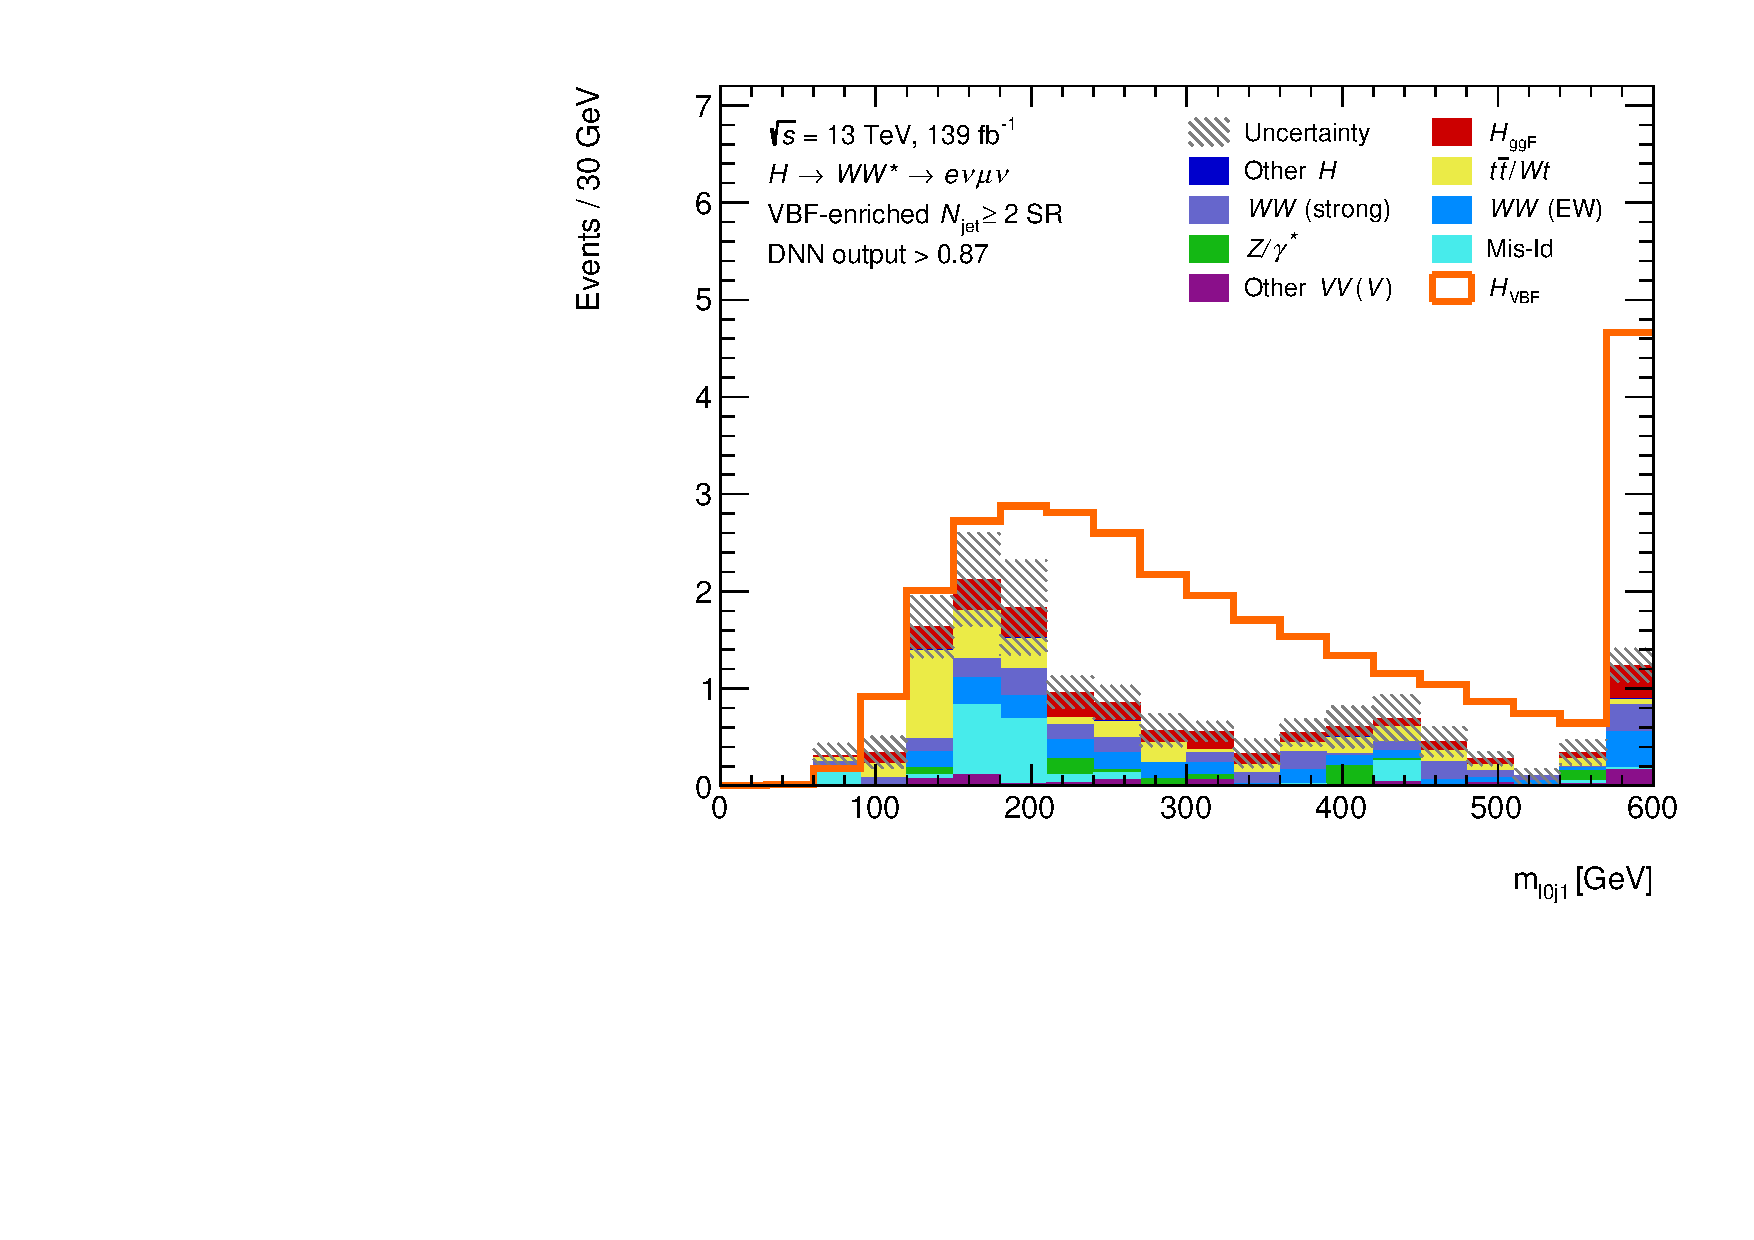
\includegraphics[width=0.32\textwidth]{figures/hww/dnn/blinded/run2-emme-CutVBFSR_DNN87-Ml0j1-lin.pdf}
    } \\
    \subfloat[$\mltwojtwo$]{
        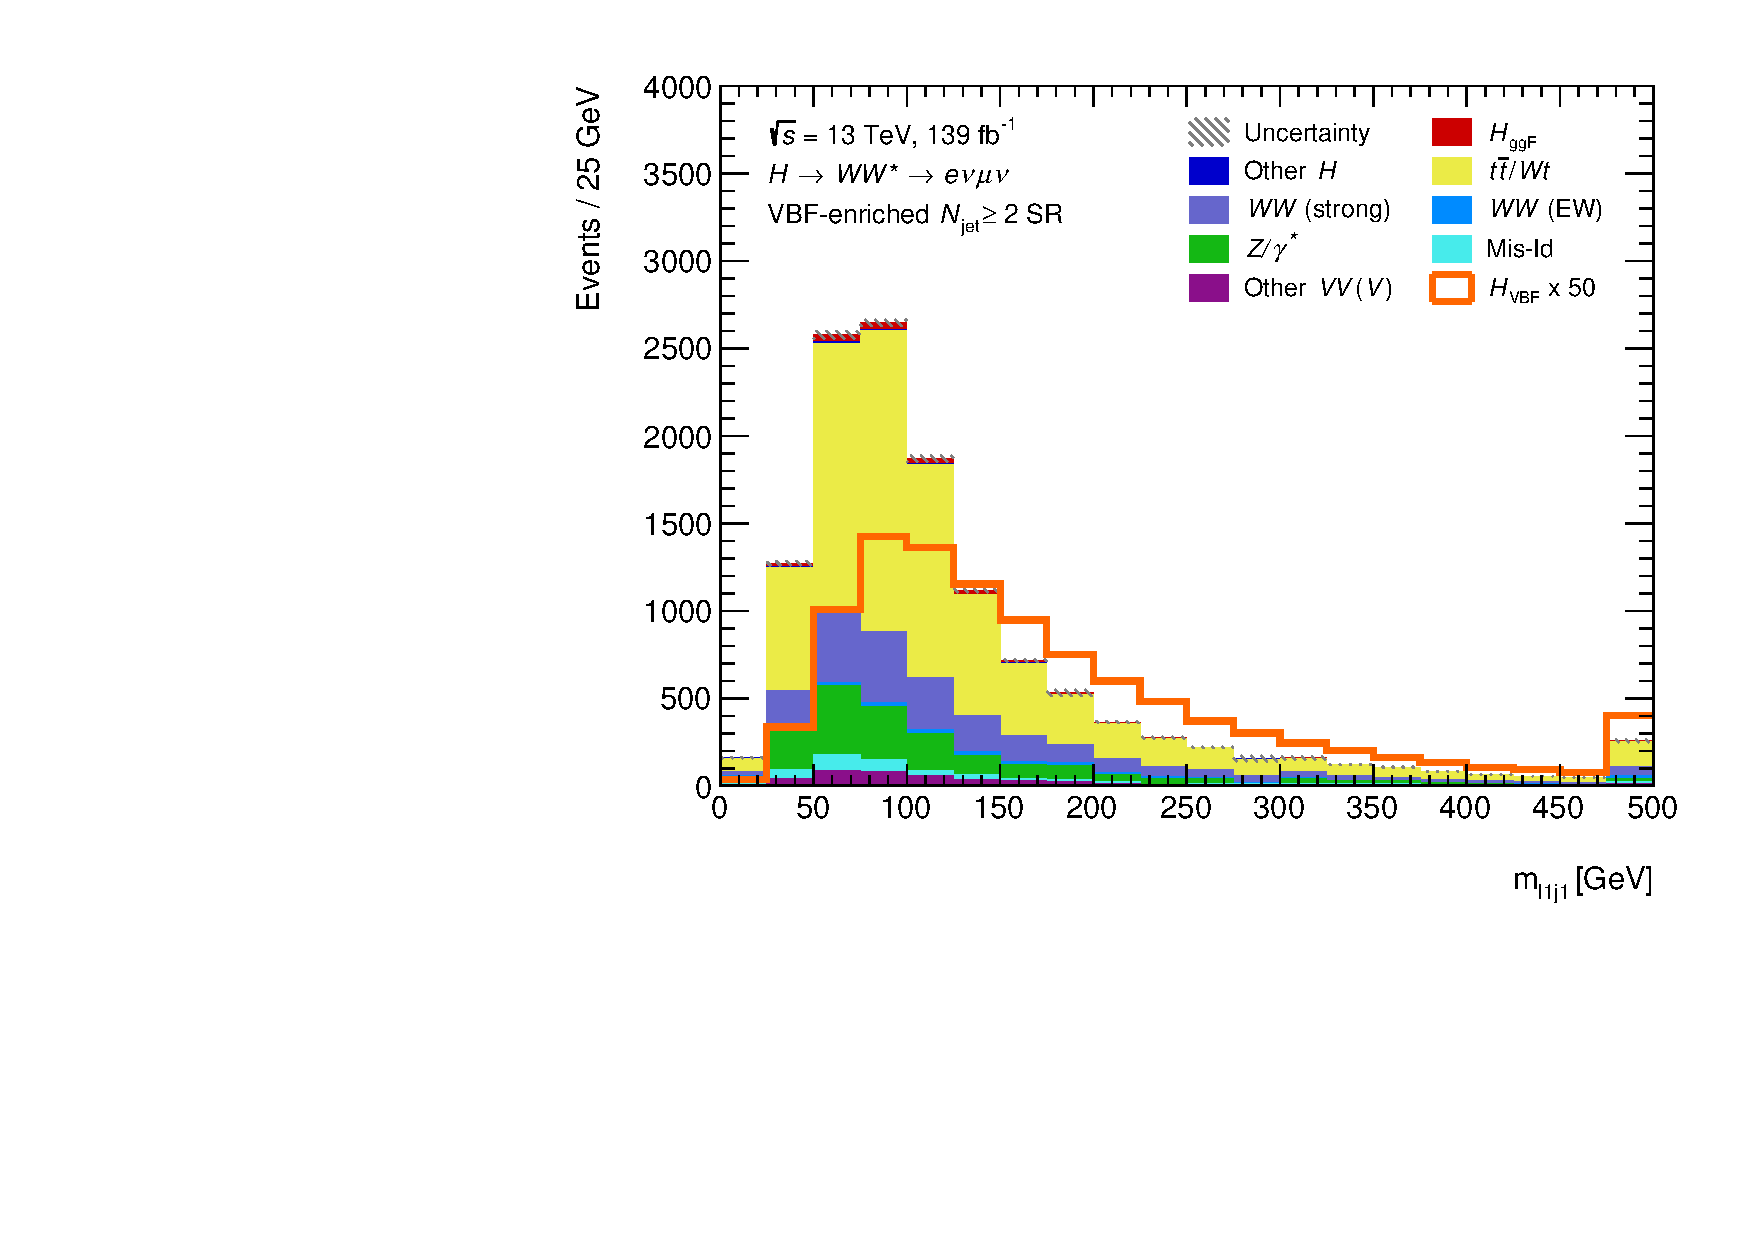
\includegraphics[width=0.32\textwidth]{figures/hww/dnn/blinded/run2-emme-CutVBF_SR-Ml1j1-lin.pdf} \hfill
        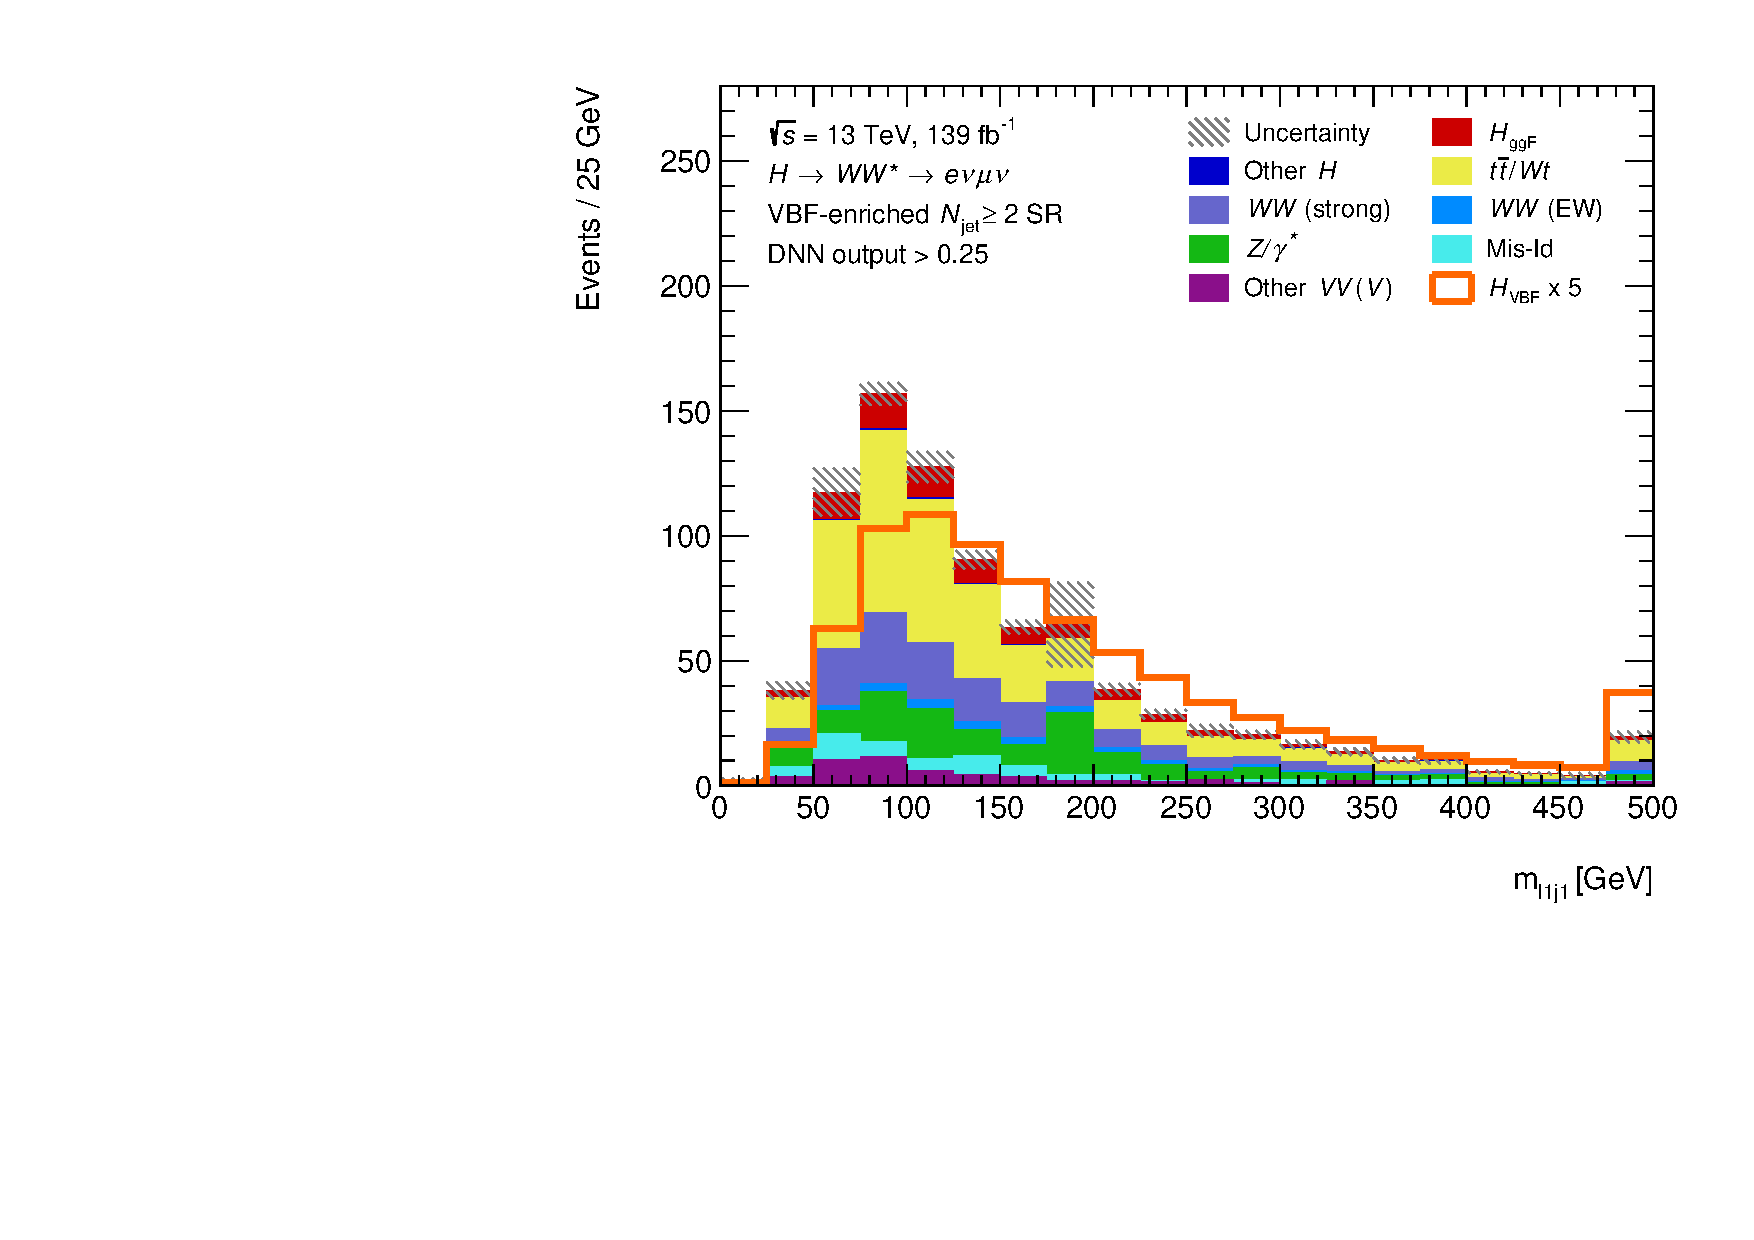
\includegraphics[width=0.32\textwidth]{figures/hww/dnn/blinded/run2-emme-CutVBFSR_DNN25-Ml1j1-lin.pdf} \hfill
        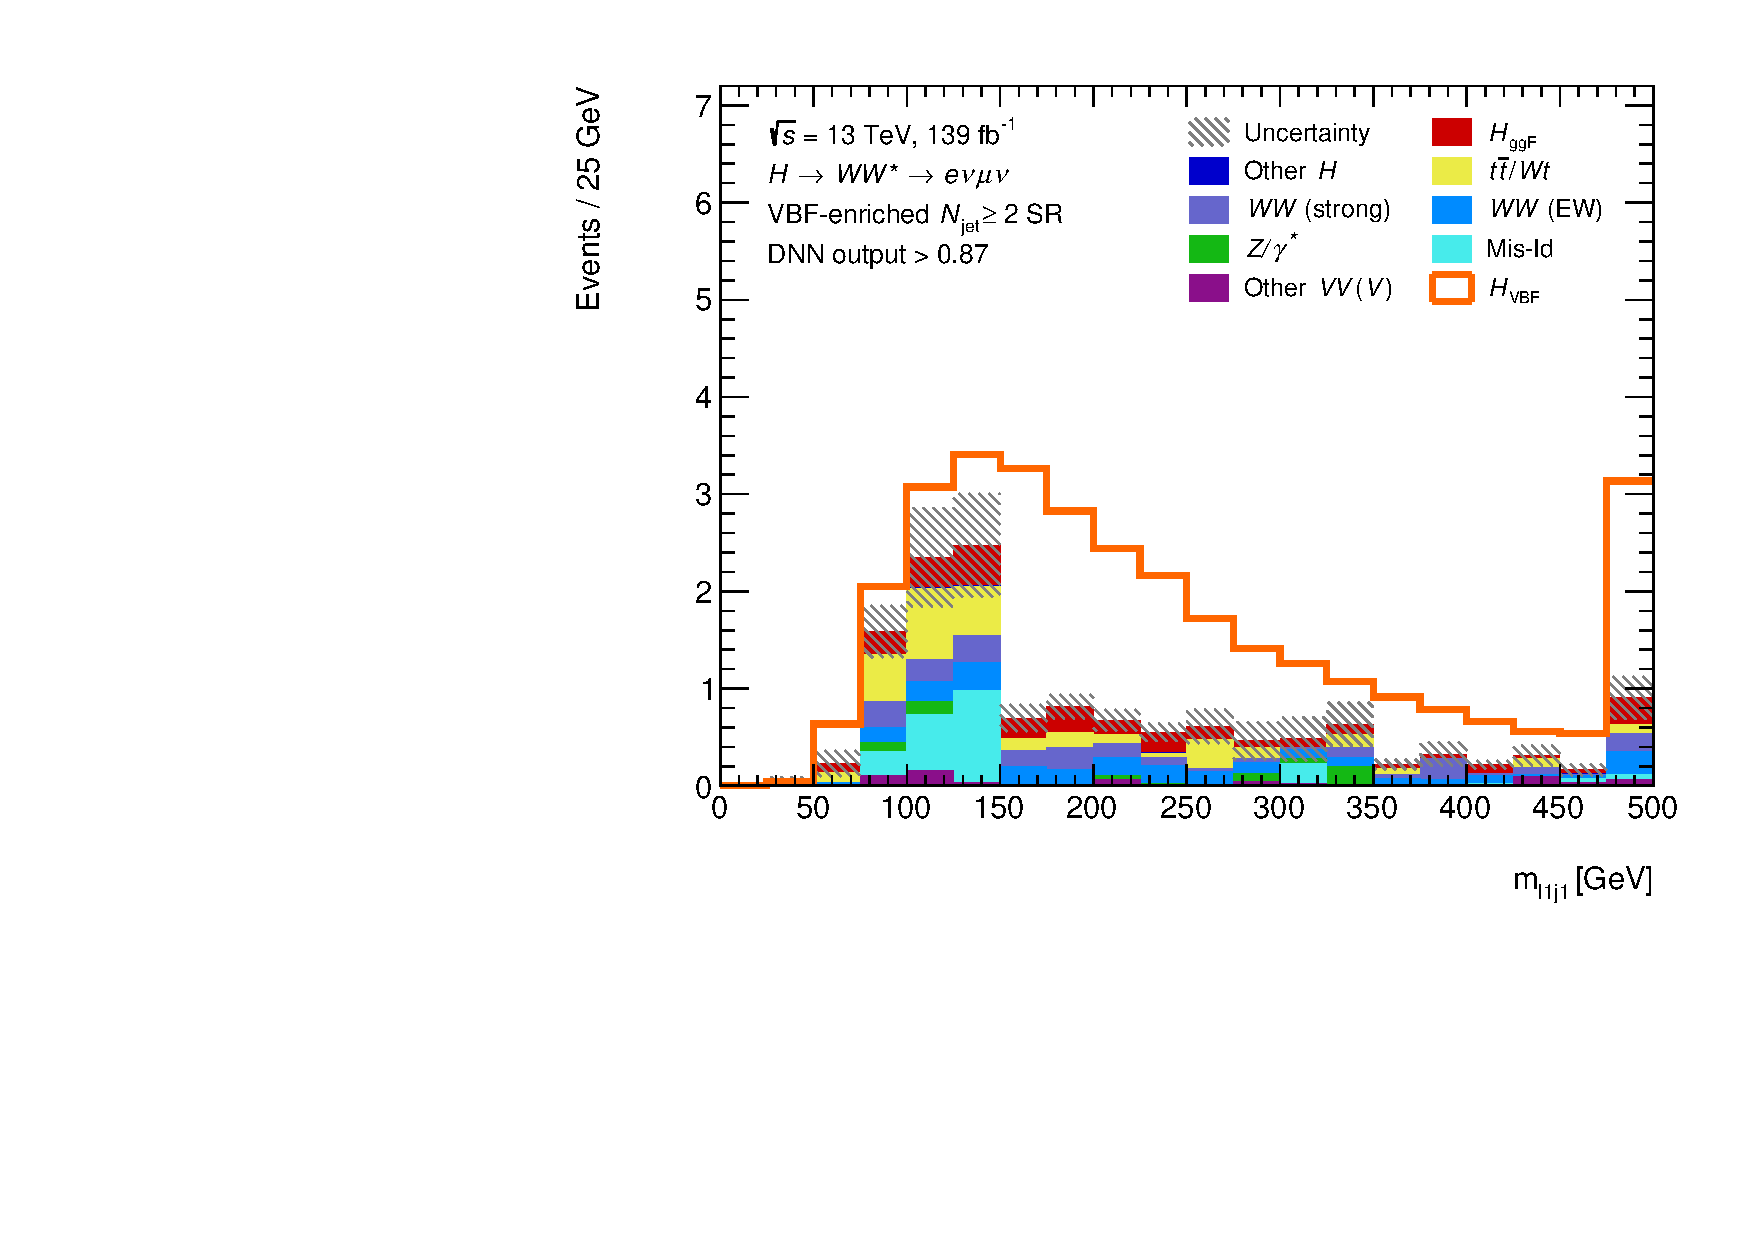
\includegraphics[width=0.32\textwidth]{figures/hww/dnn/blinded/run2-emme-CutVBFSR_DNN87-Ml1j1-lin.pdf}
    } 
    {\caption{Distributions of $\mlonejone$, $\mltwojone$, $\mlonejtwo$, and $\mltwojtwo$ in the VBF signal region.
            Each row shows one variable with different cuts on the DNN output distribution being applied in different columns.
            \label{fig:dnn-inputs-vbf-top2} }}
\end{figure}


\begin{figure}[h]
    \centering
    \subfloat[$\pTjone$]{
        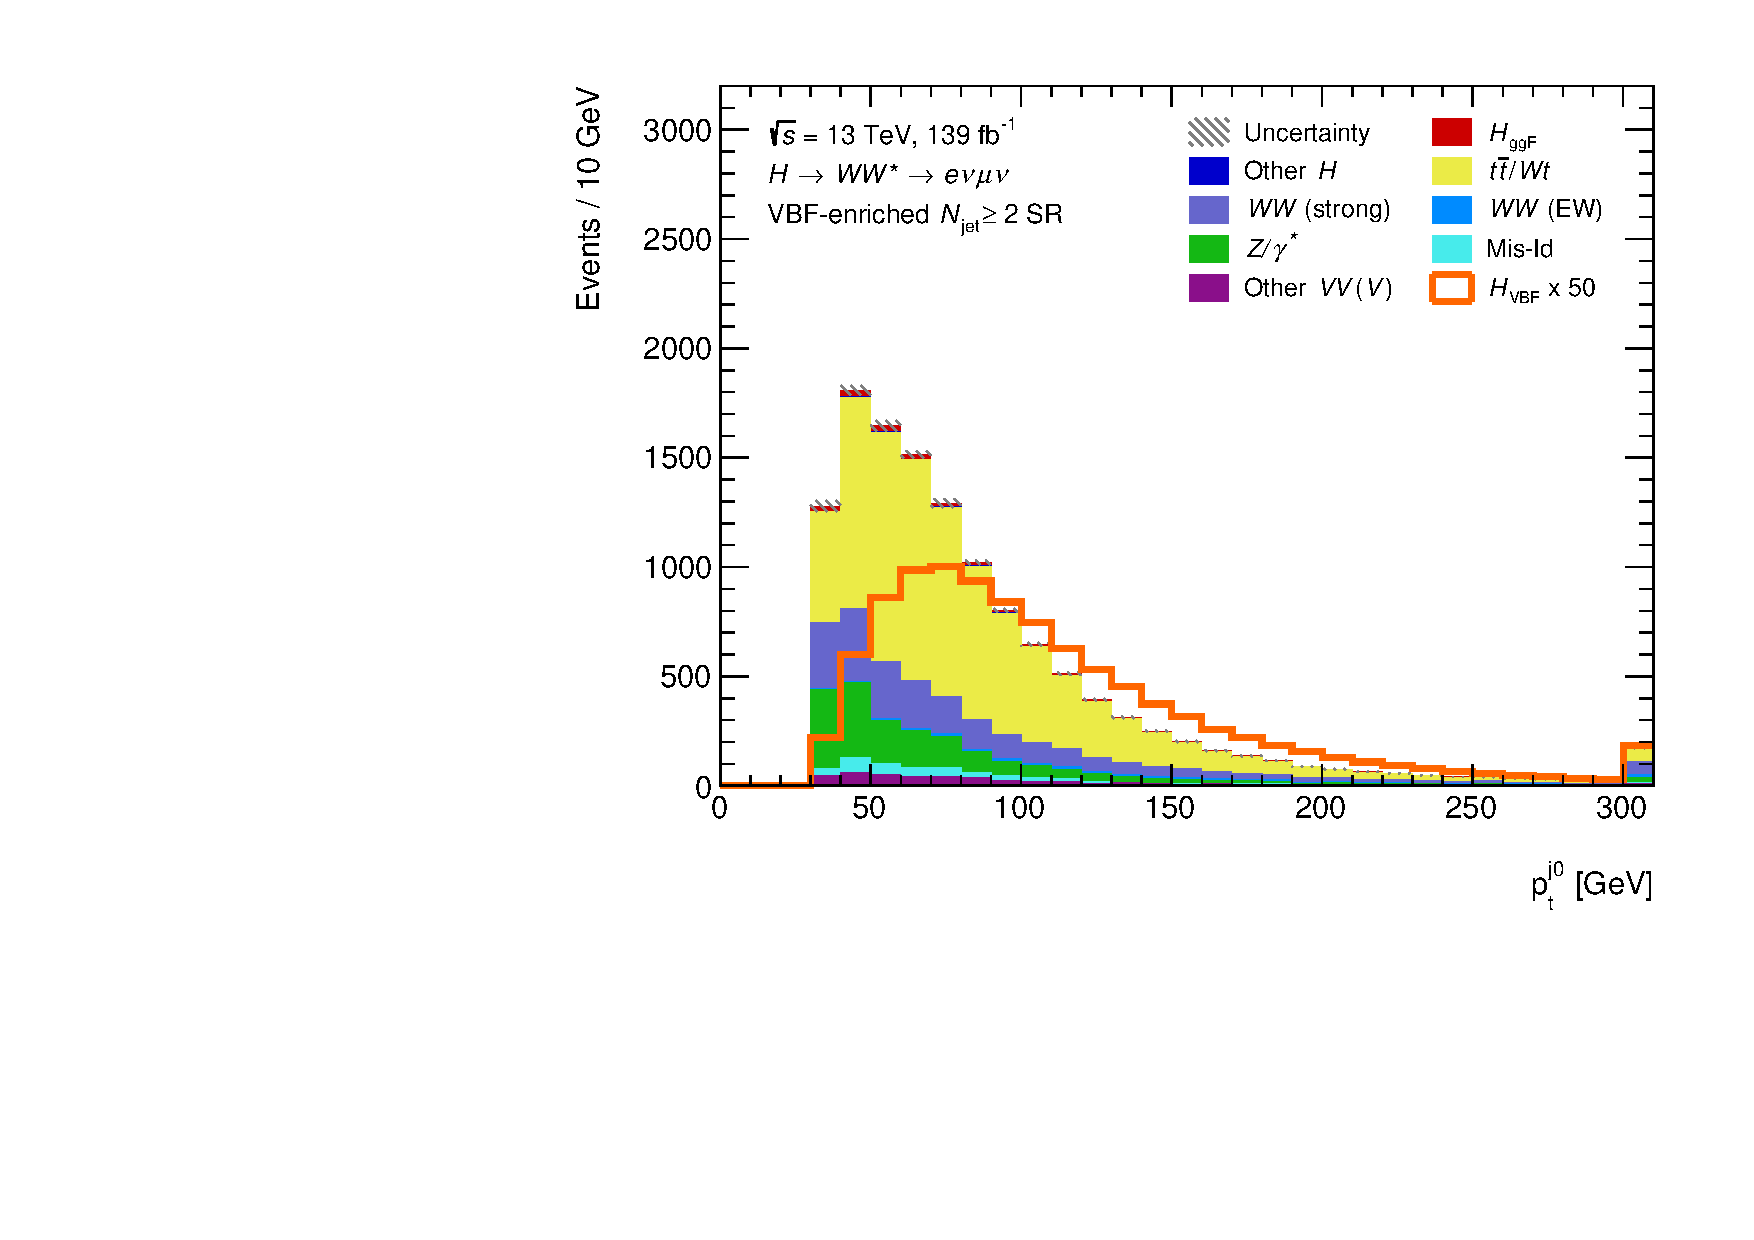
\includegraphics[width=0.32\textwidth]{figures/hww/dnn/blinded/run2-emme-CutVBF_SR-leadJetPt-lin.pdf} \hfill
        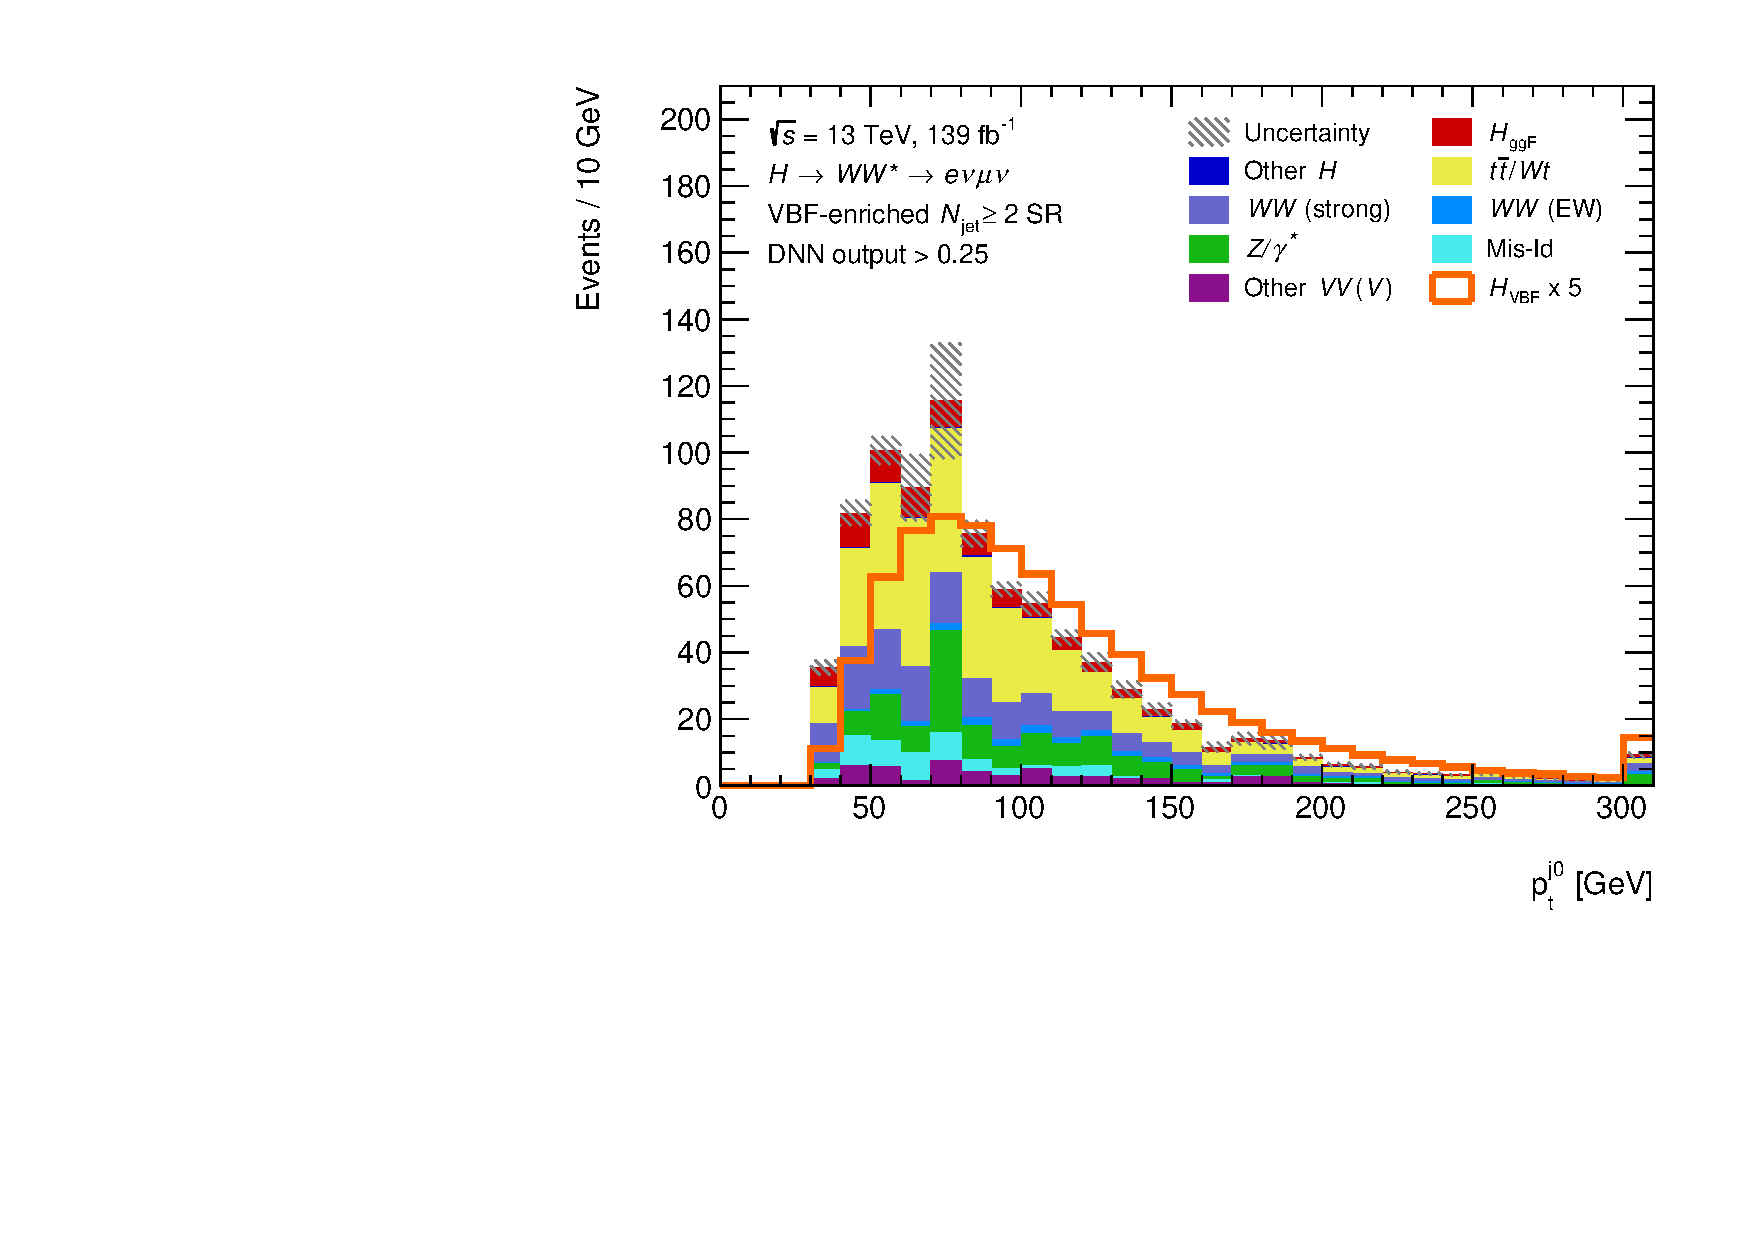
\includegraphics[width=0.32\textwidth]{figures/hww/dnn/blinded/run2-emme-CutVBFSR_DNN25-leadJetPt-lin.pdf} \hfill
        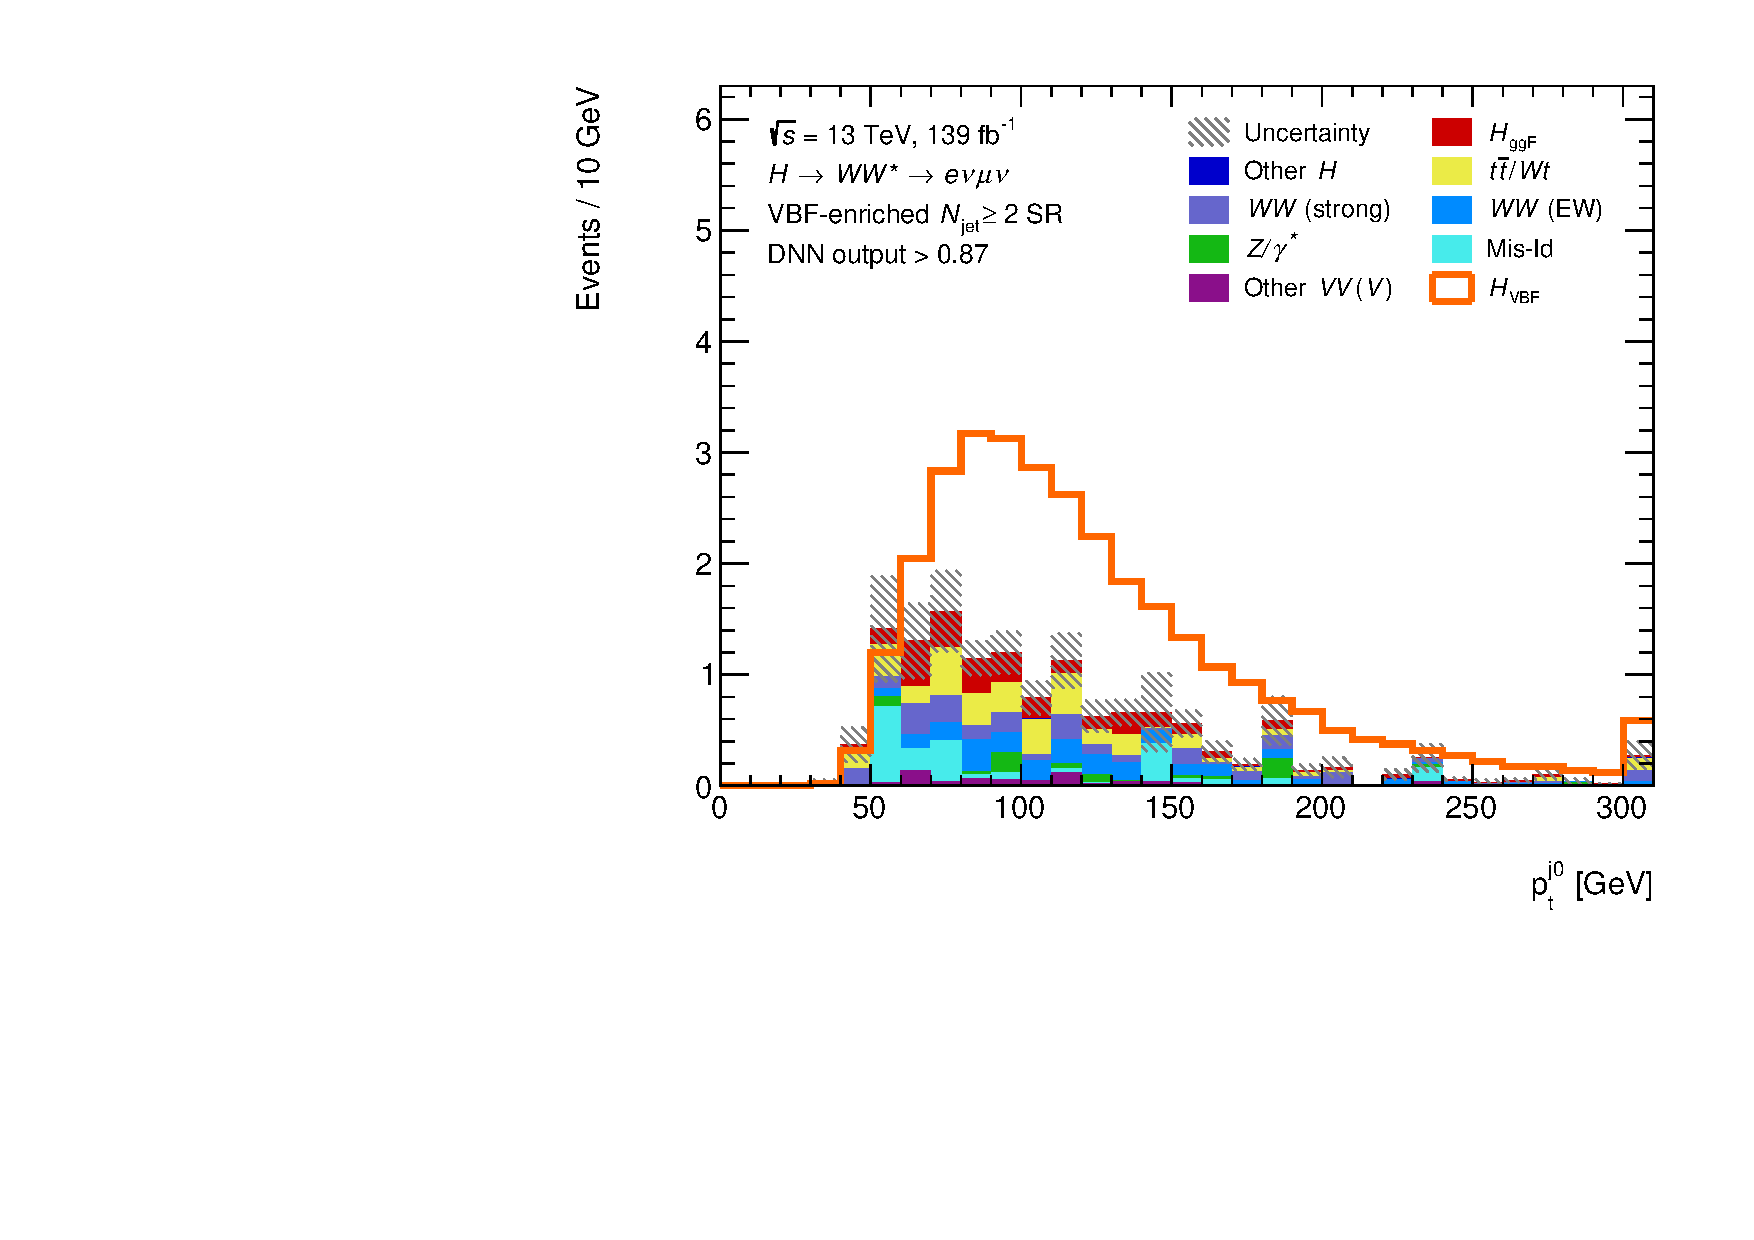
\includegraphics[width=0.32\textwidth]{figures/hww/dnn/blinded/run2-emme-CutVBFSR_DNN87-leadJetPt-lin.pdf}
    } \\
    \subfloat[$\pTjtwo$]{
        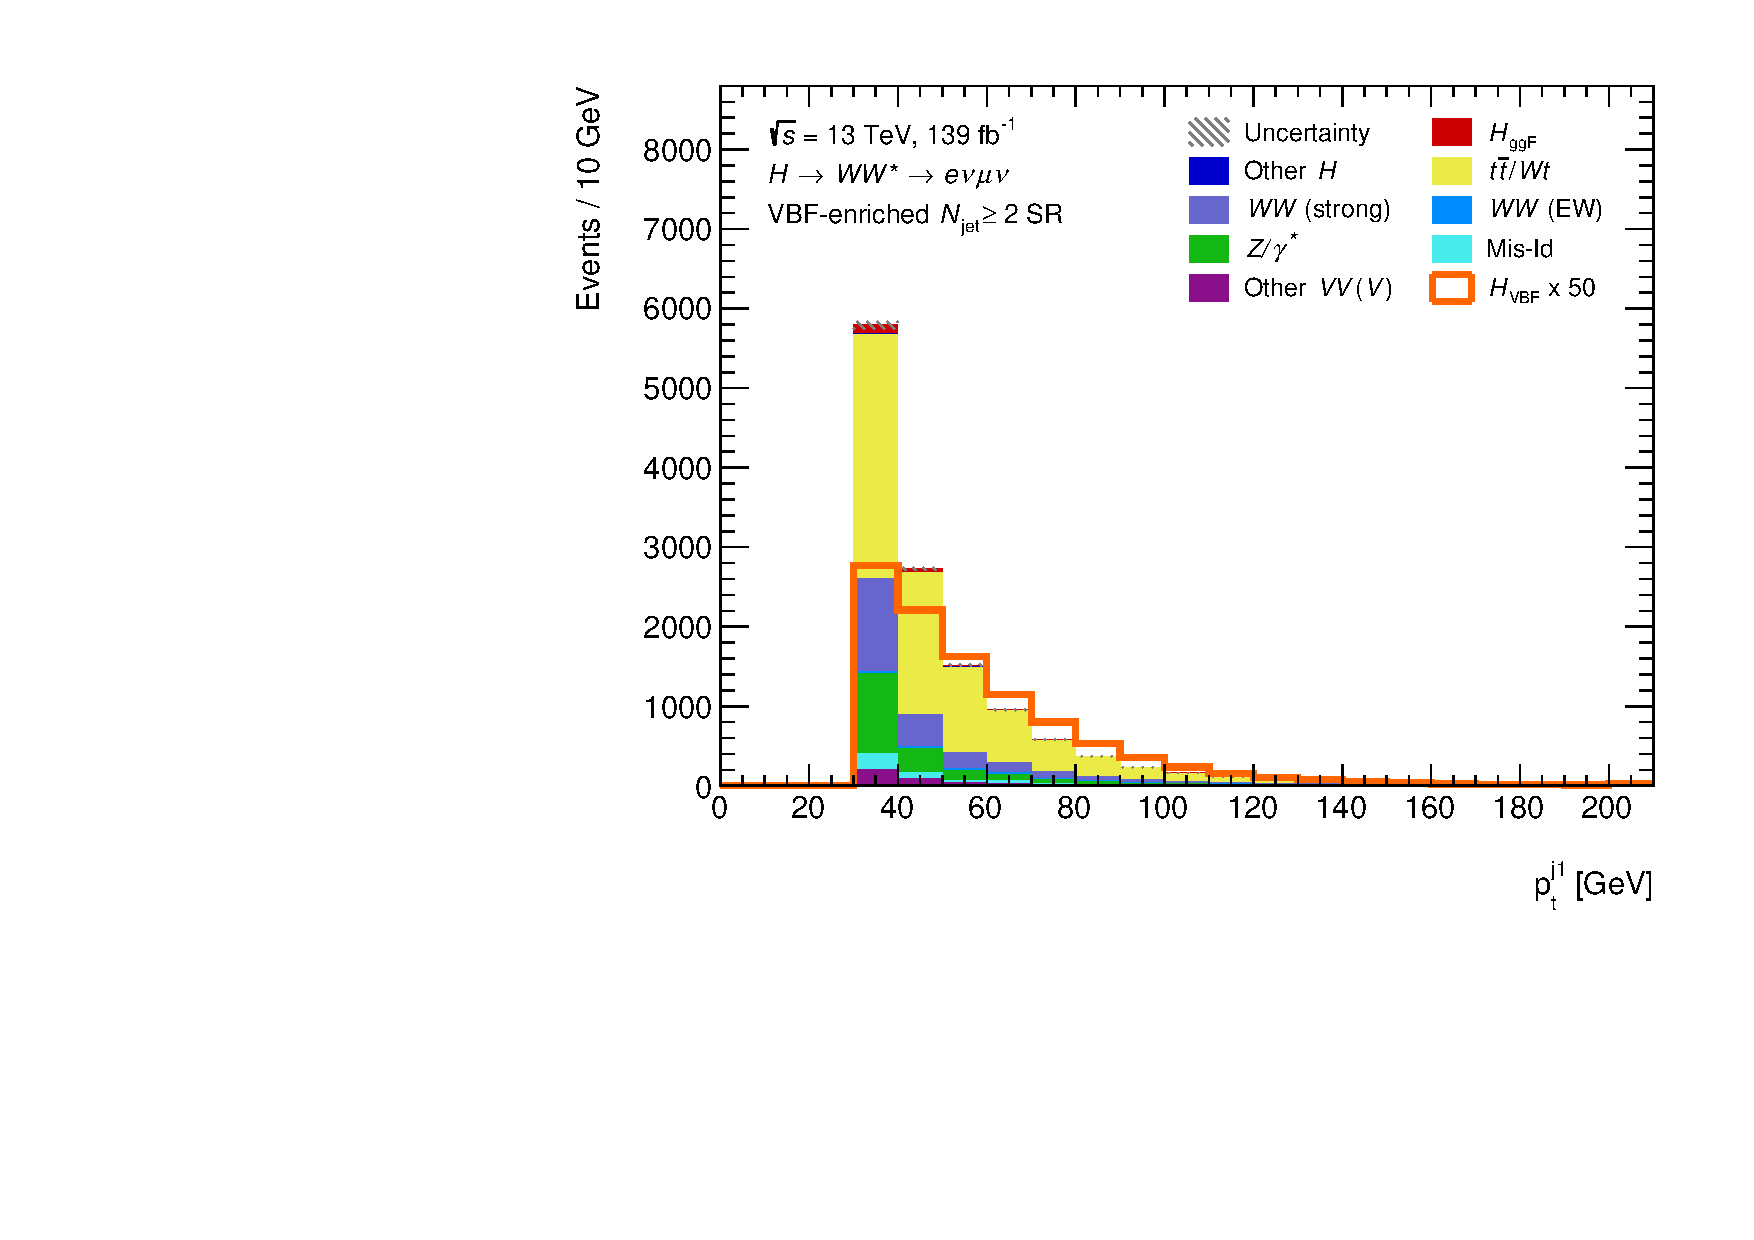
\includegraphics[width=0.32\textwidth]{figures/hww/dnn/blinded/run2-emme-CutVBF_SR-subleadJetPt-lin.pdf} \hfill
        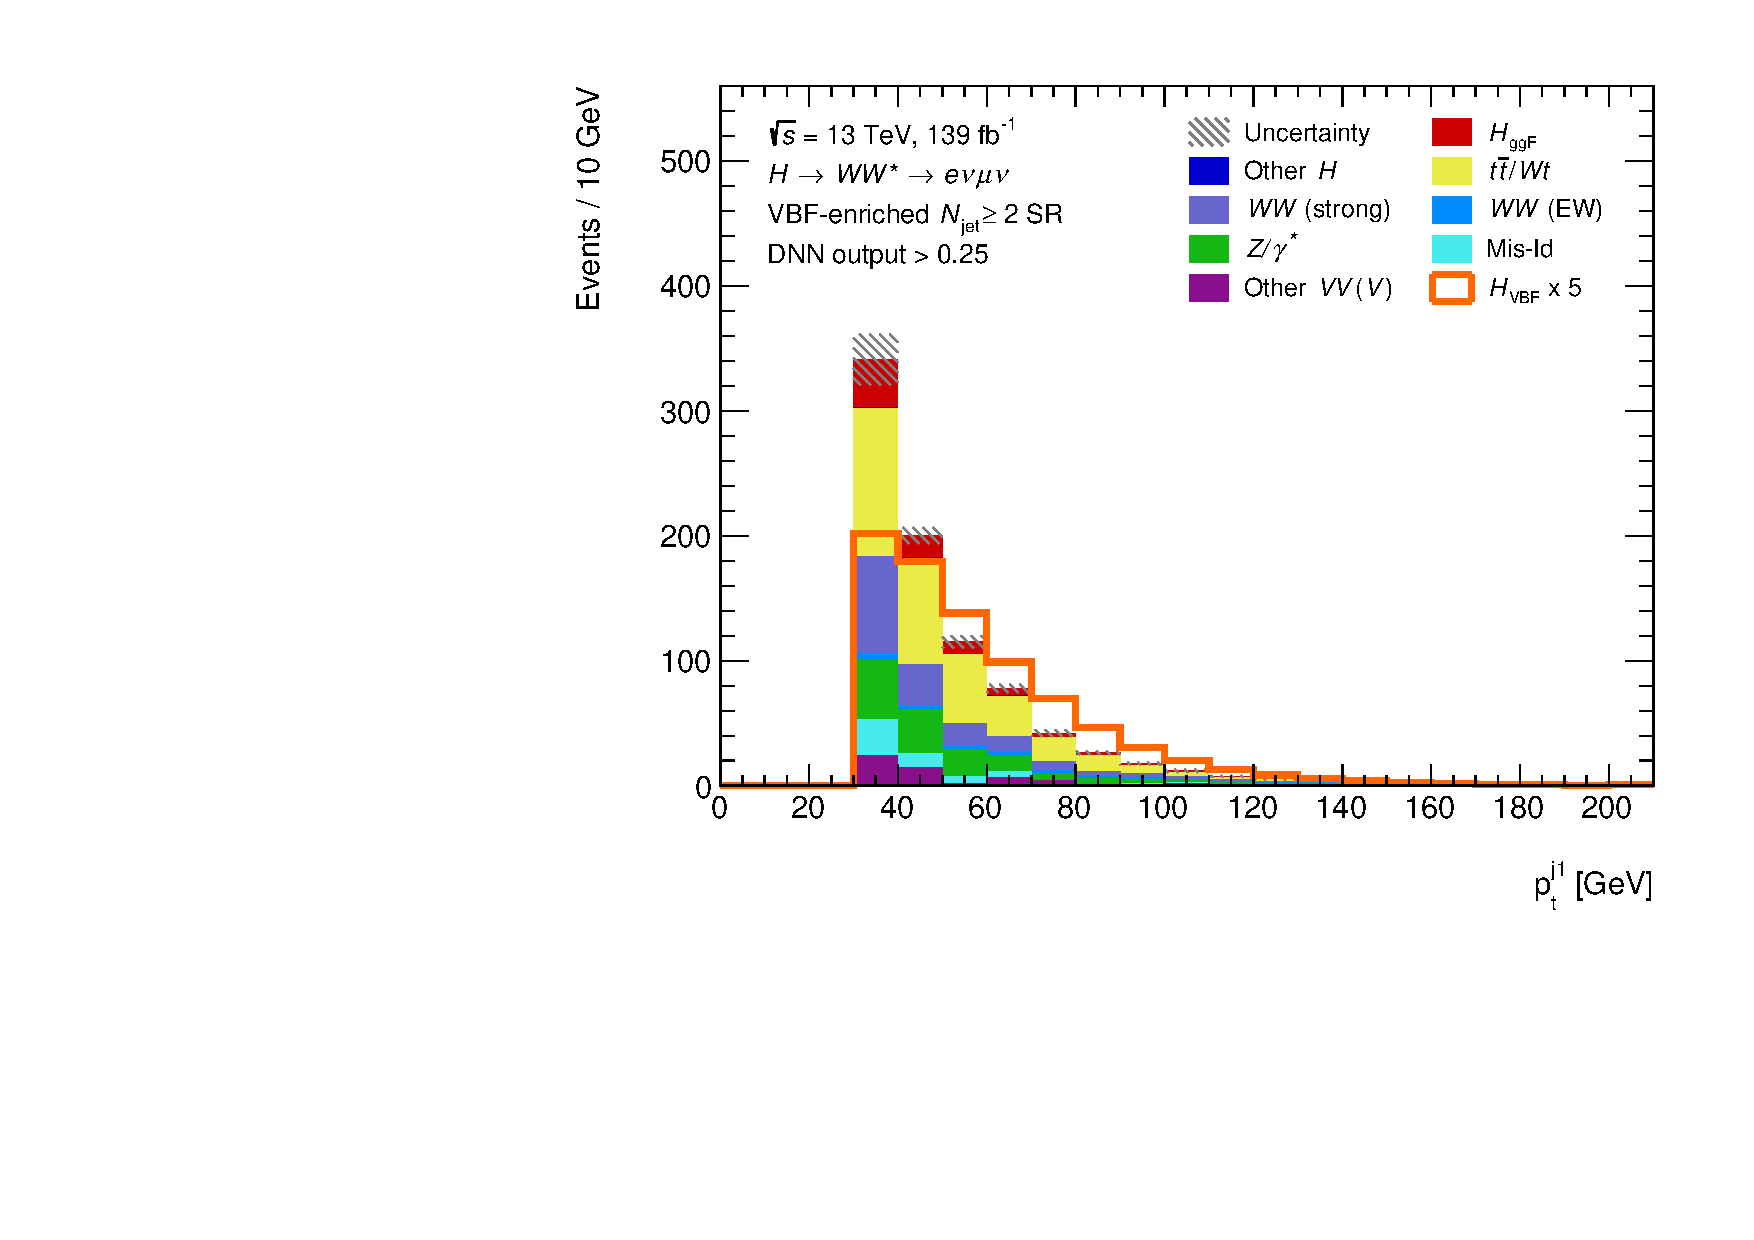
\includegraphics[width=0.32\textwidth]{figures/hww/dnn/blinded/run2-emme-CutVBFSR_DNN25-subleadJetPt-lin.pdf} \hfill
        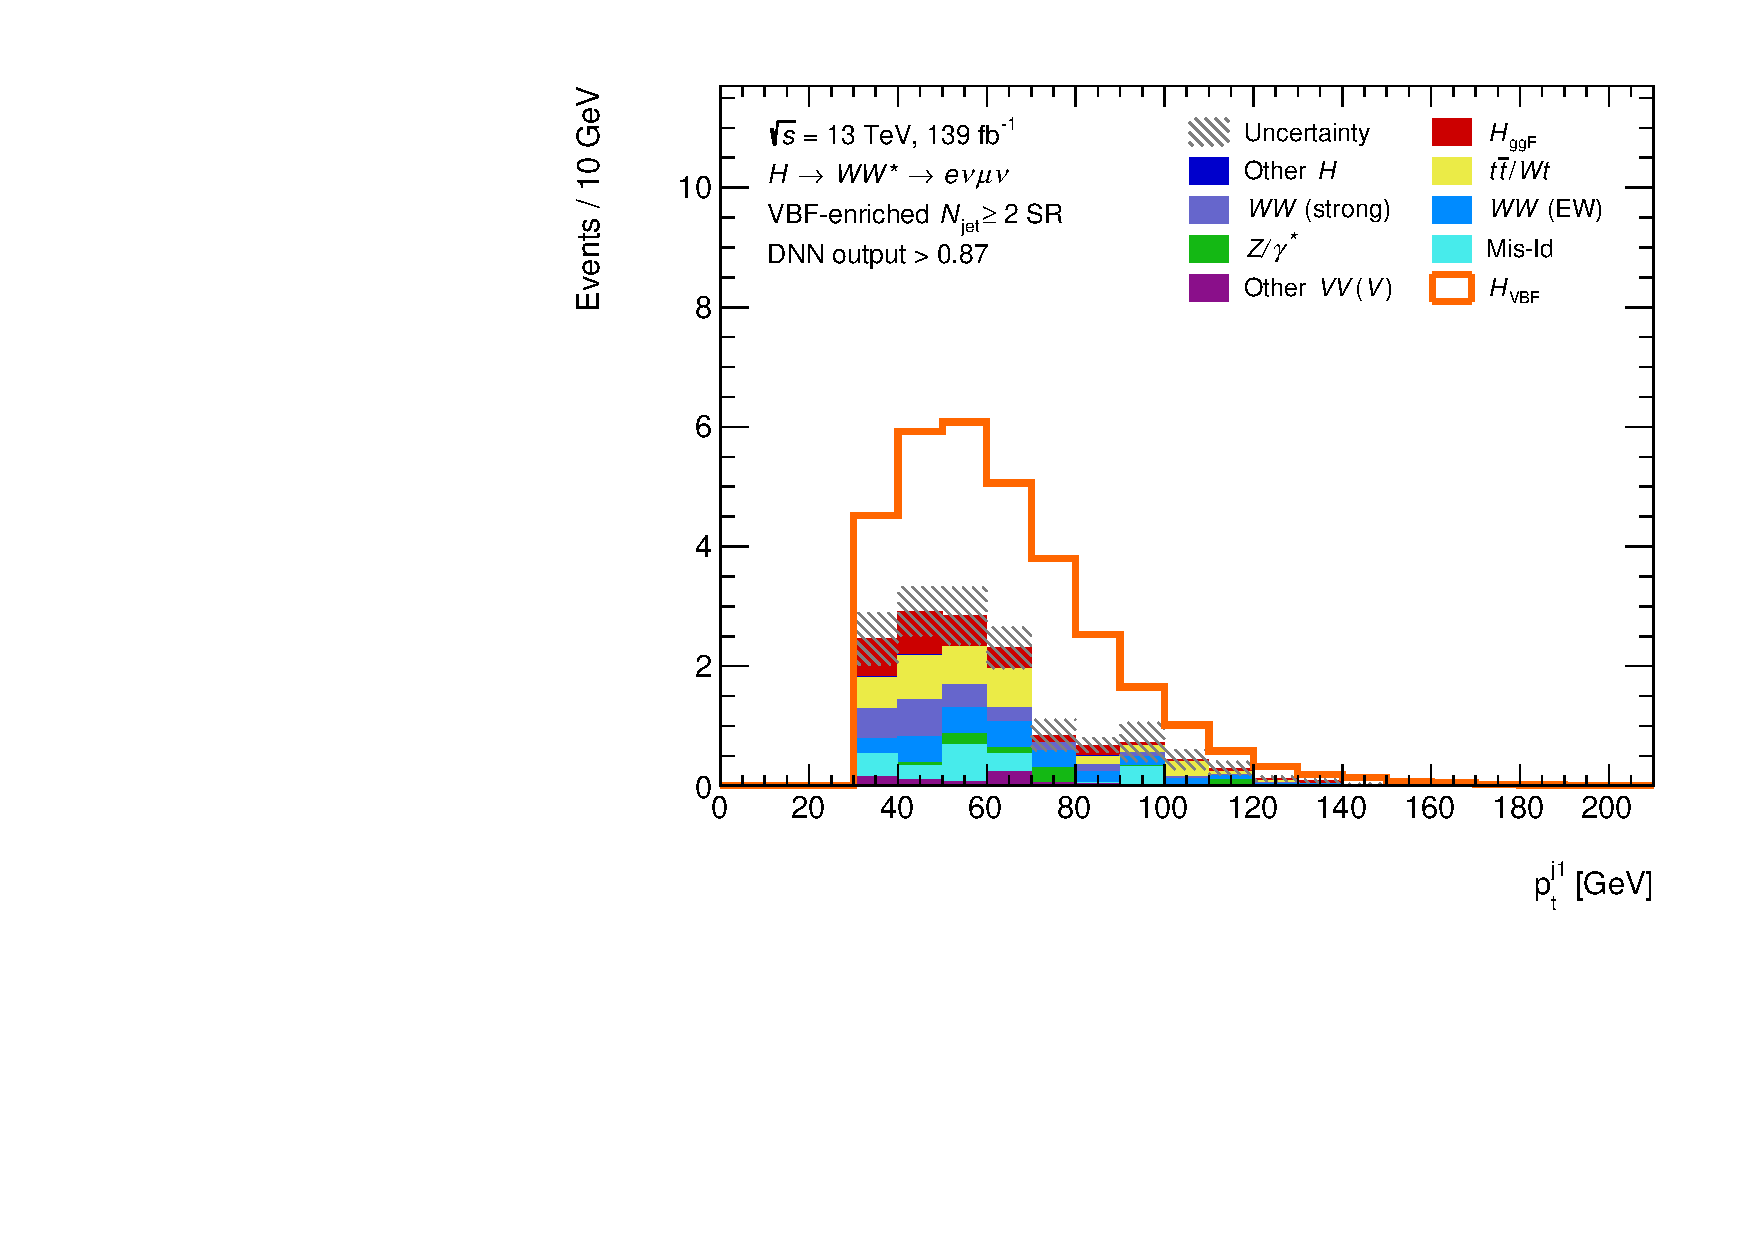
\includegraphics[width=0.32\textwidth]{figures/hww/dnn/blinded/run2-emme-CutVBFSR_DNN87-subleadJetPt-lin.pdf}
    } \\
    \subfloat[$\pTjthree$]{
        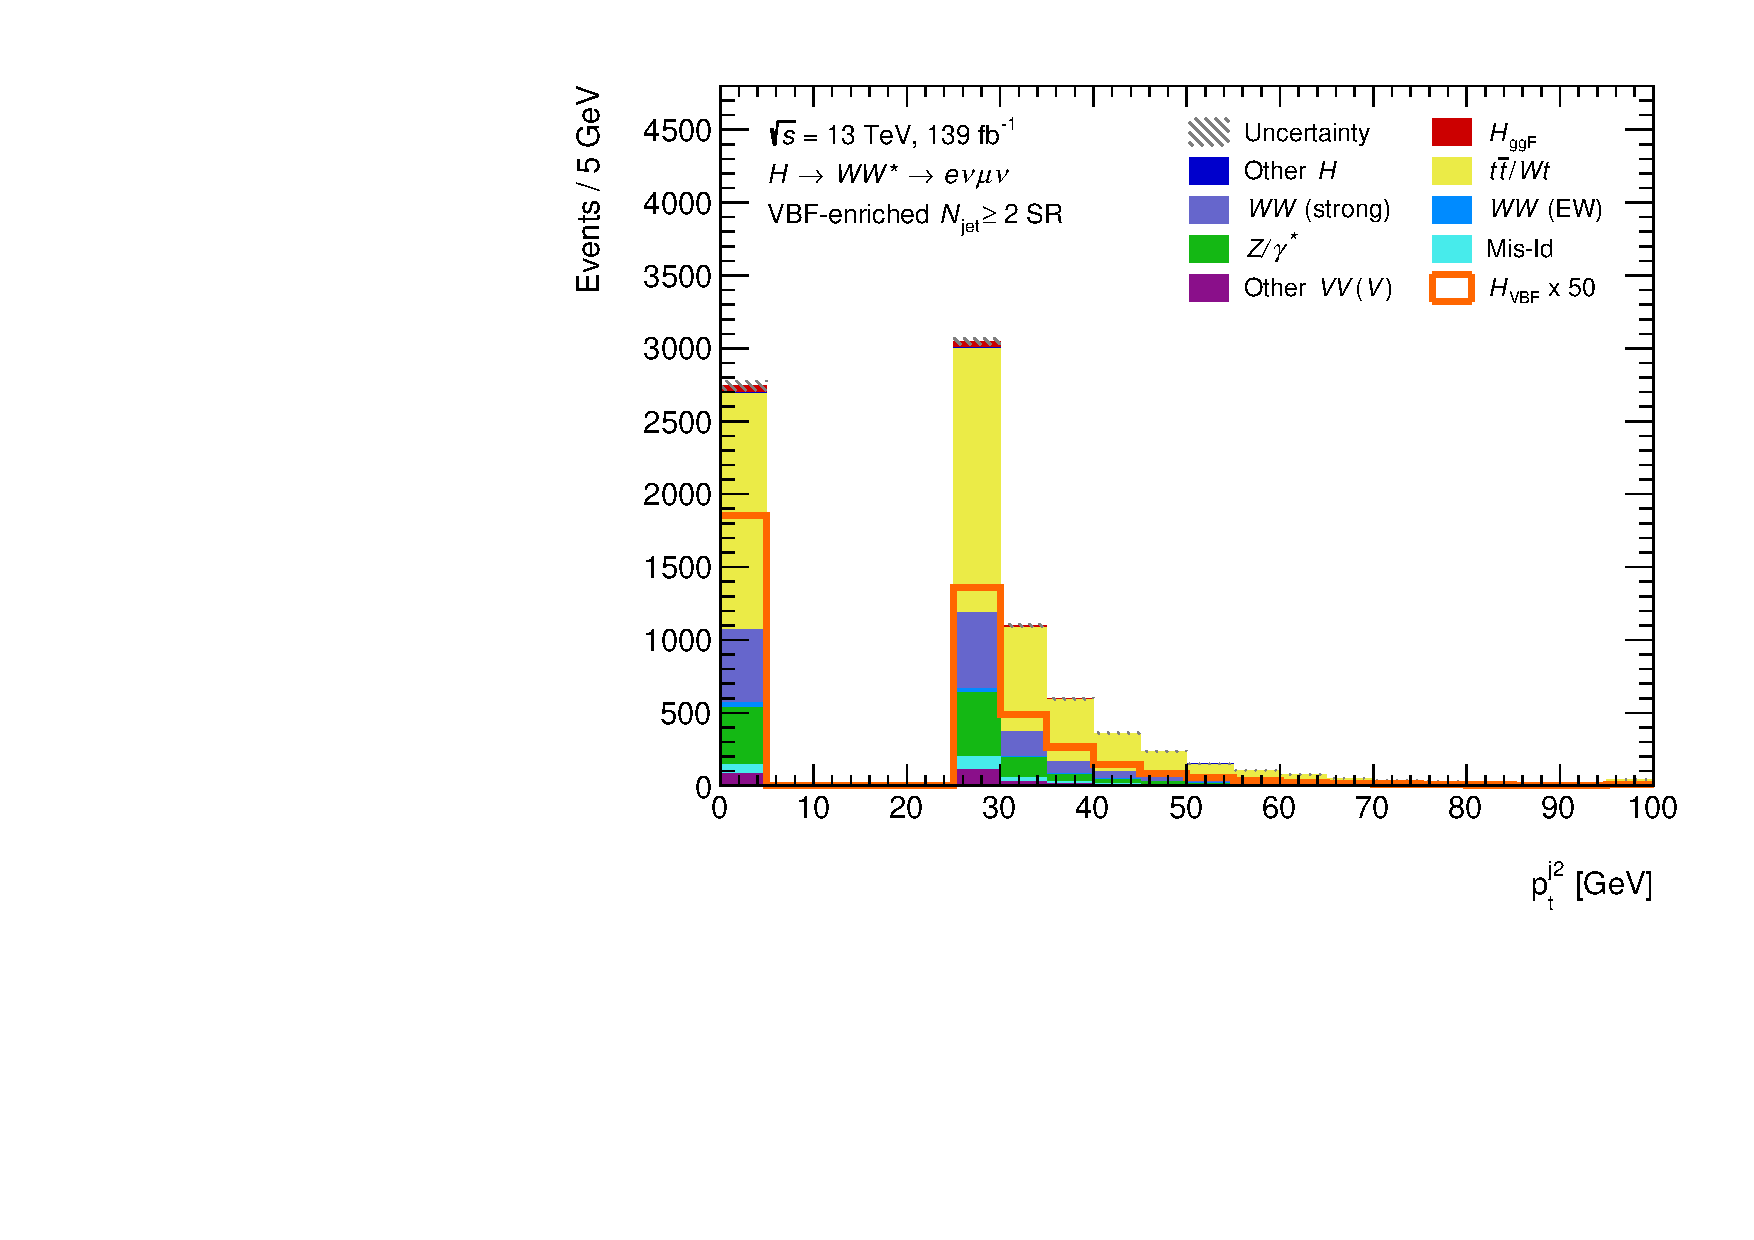
\includegraphics[width=0.32\textwidth]{figures/hww/dnn/blinded/run2-emme-CutVBF_SR-thirdJetPt-lin.pdf} \hfill
        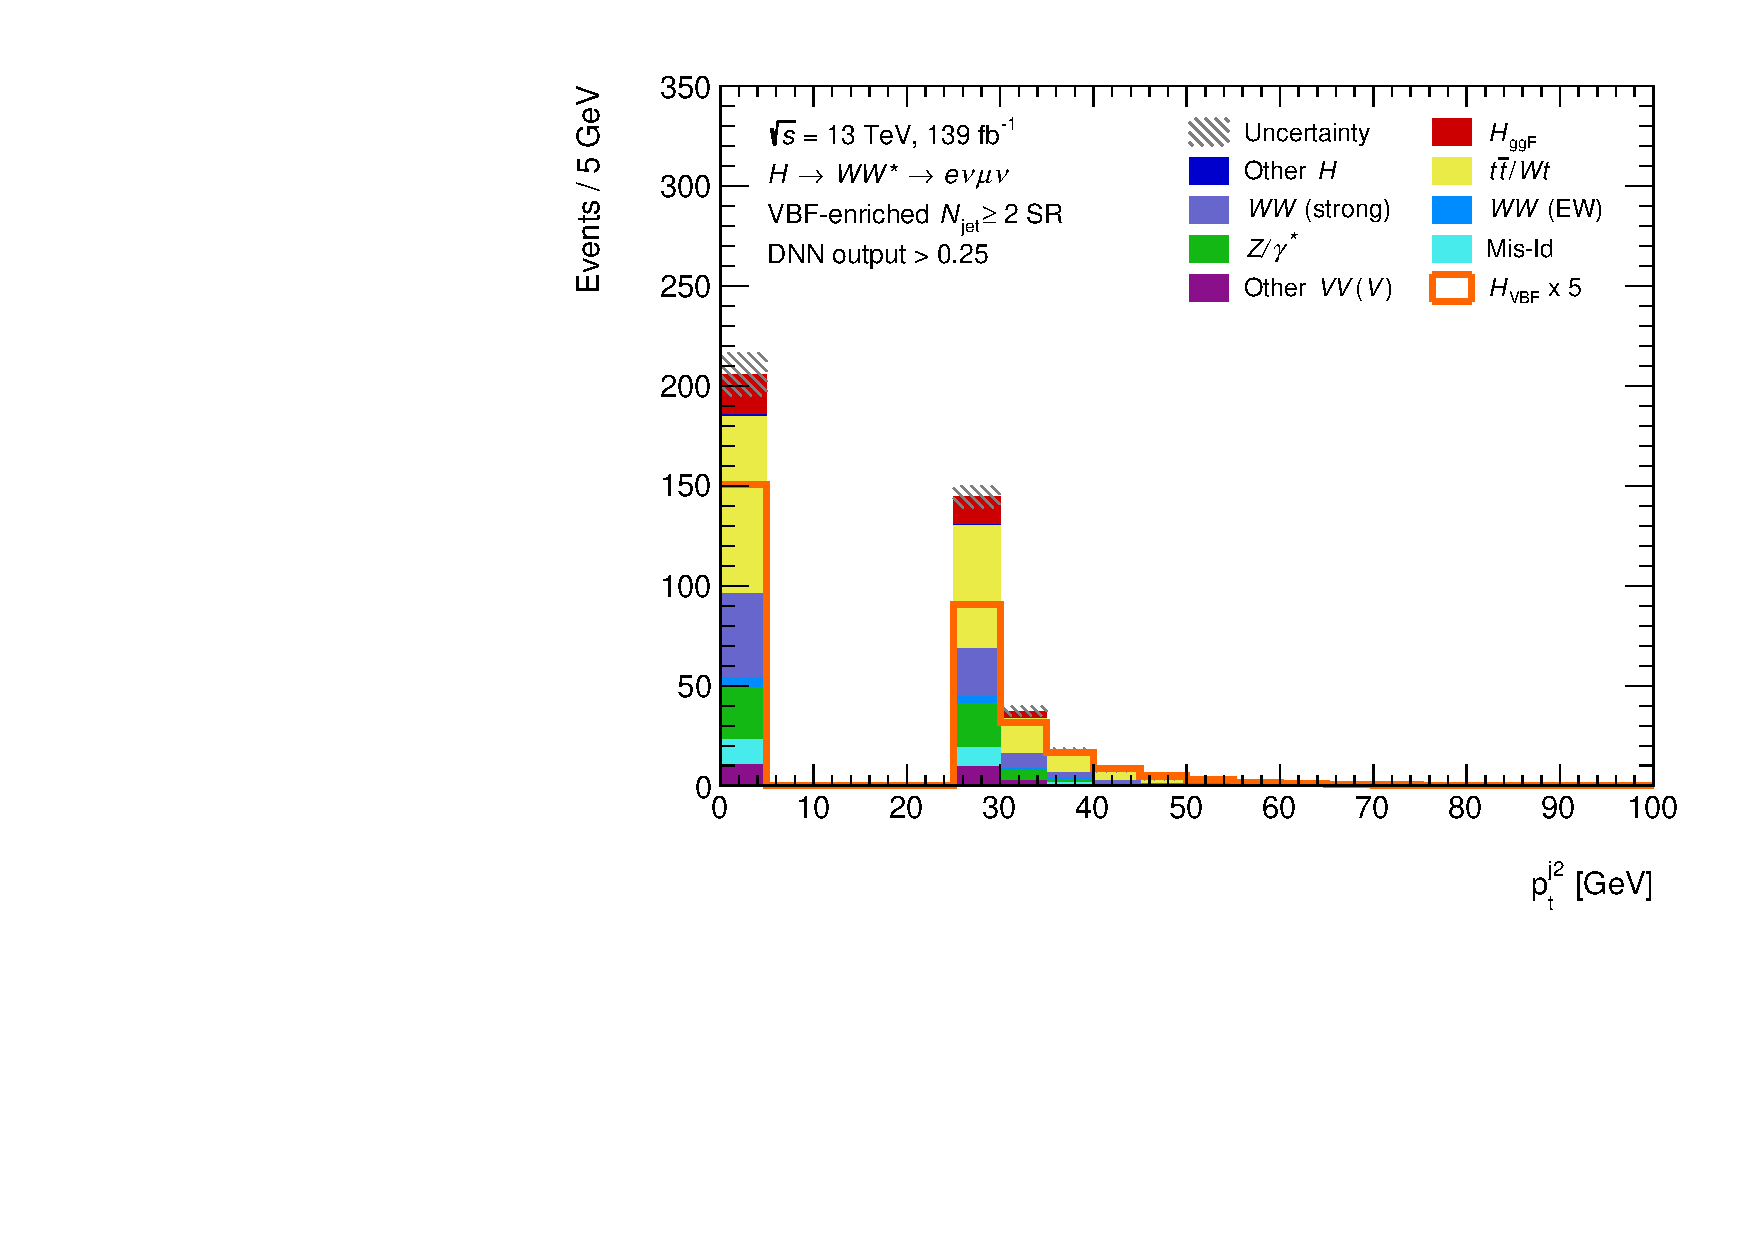
\includegraphics[width=0.32\textwidth]{figures/hww/dnn/blinded/run2-emme-CutVBFSR_DNN25-thirdJetPt-lin.pdf} \hfill
        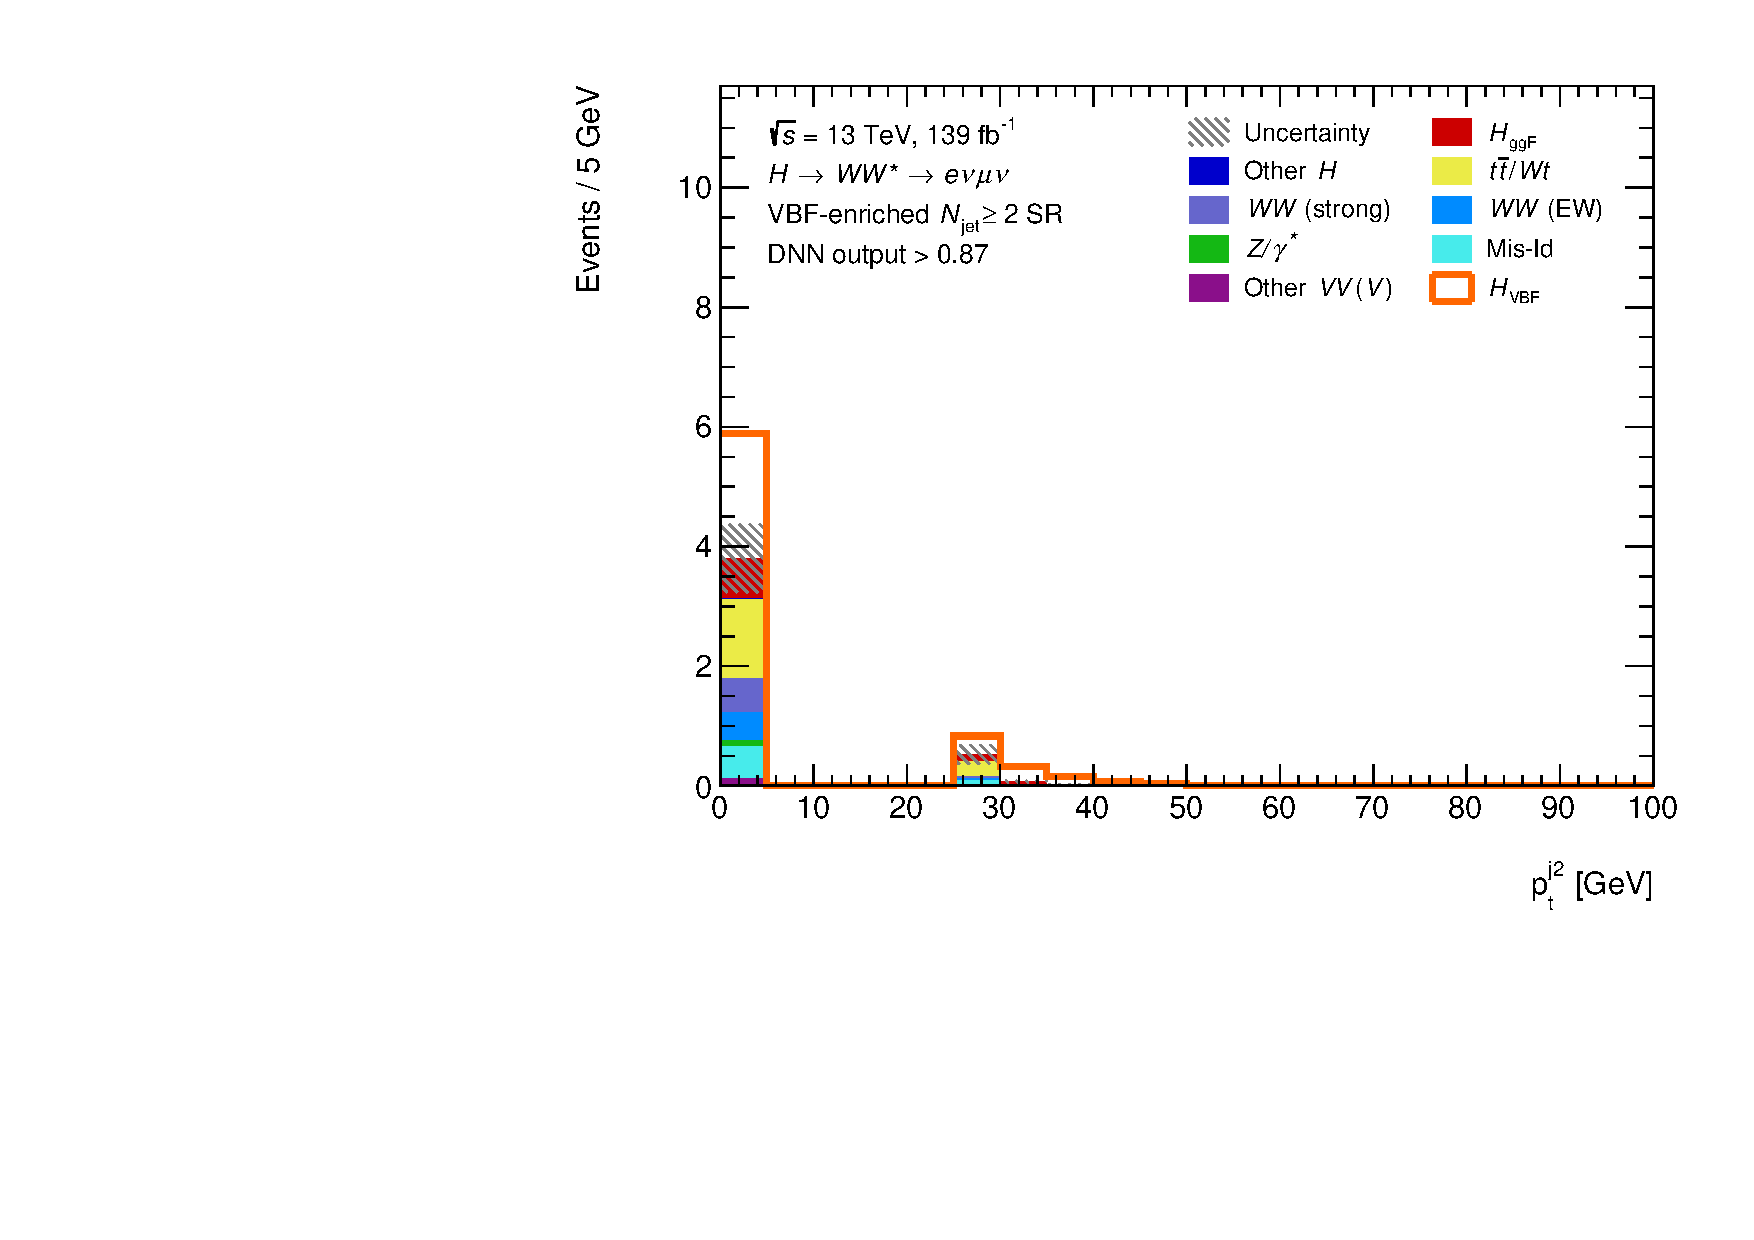
\includegraphics[width=0.32\textwidth]{figures/hww/dnn/blinded/run2-emme-CutVBFSR_DNN87-thirdJetPt-lin.pdf}
    } 
    {\caption{Distributions of $\pTjone$, $\pTjtwo$, and $\pTjthree$ in the VBF signal region.
            Each row shows one variable with different cuts on the DNN output distribution being applied in different columns.
            \label{fig:dnn-inputs-vbf-top3}}}
\end{figure}


\begin{figure}[h]
    \centering
    \subfloat[$\dphill$]{
        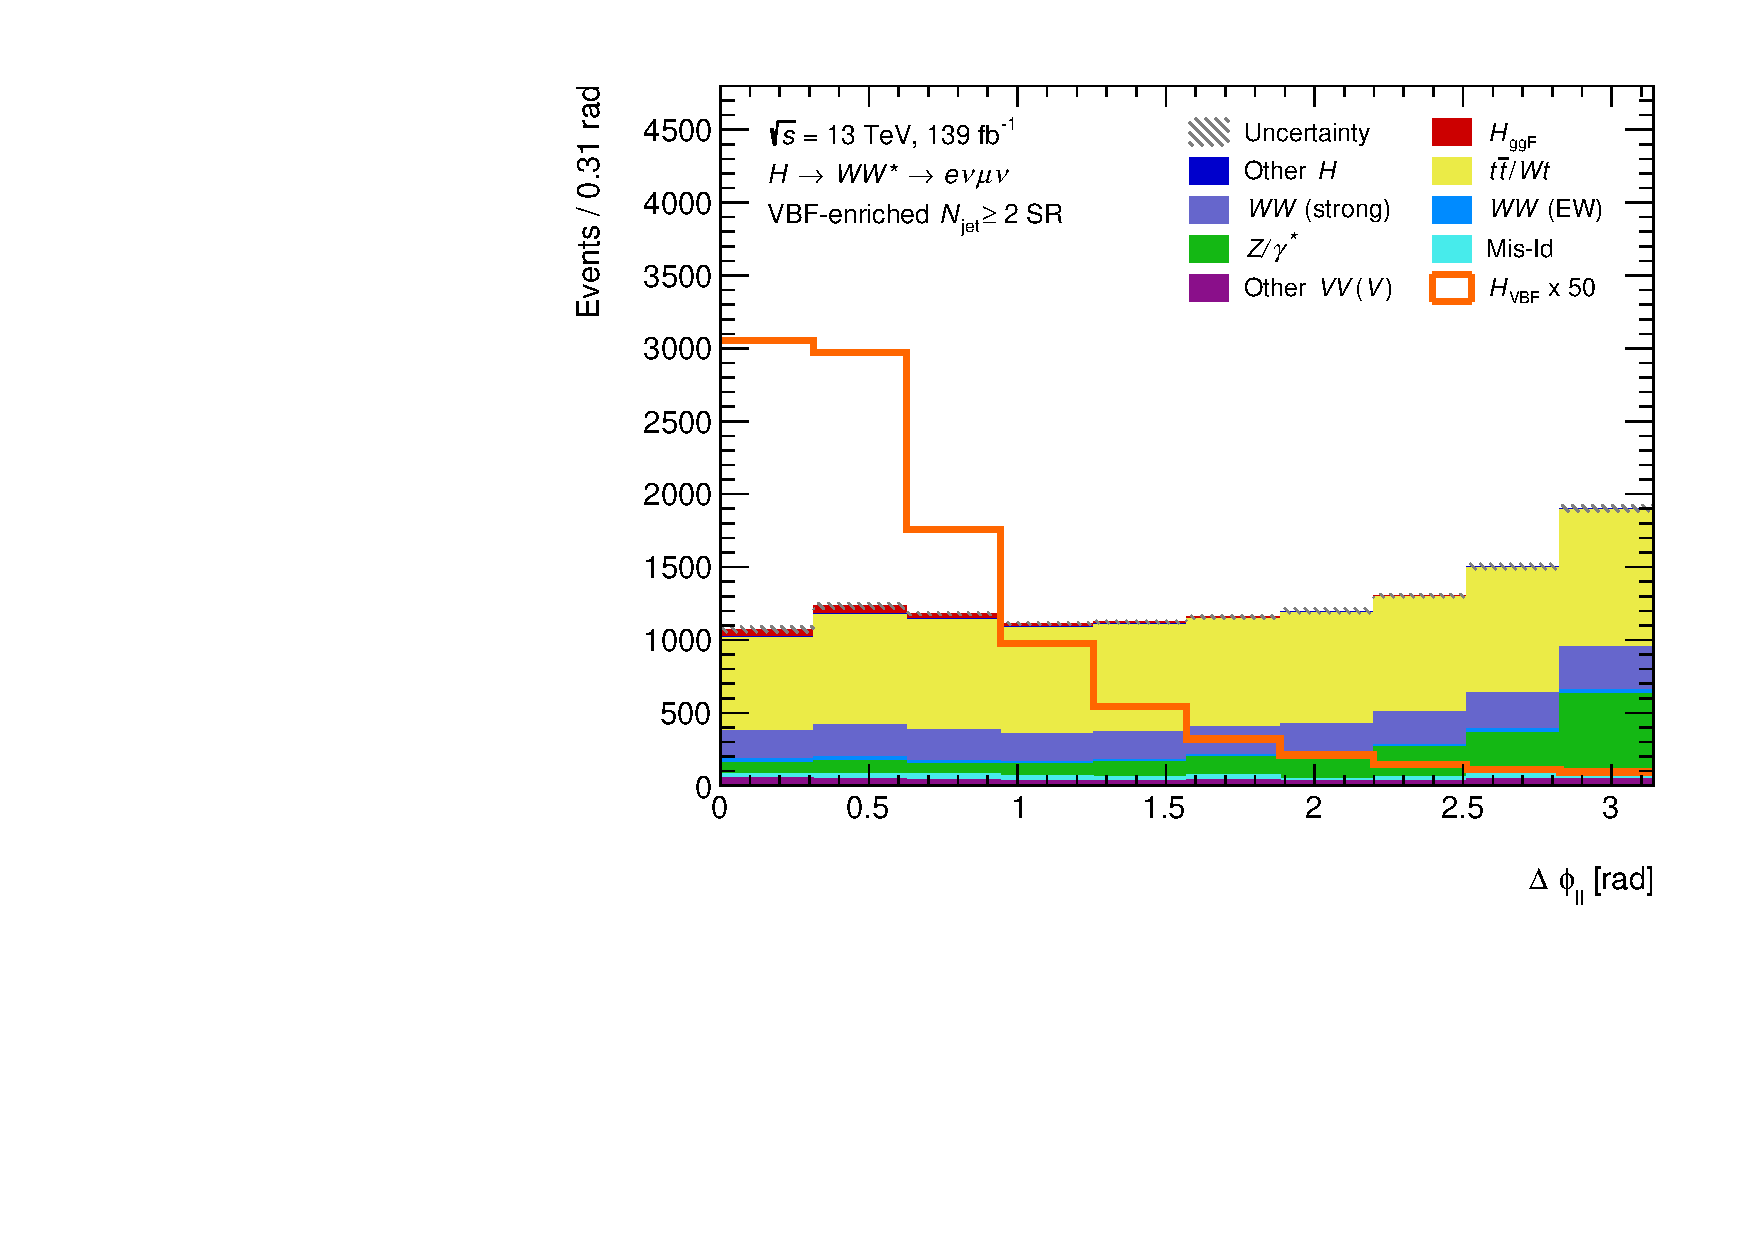
\includegraphics[width=0.32\textwidth]{figures/hww/dnn/blinded/run2-emme-CutVBF_SR-DPhill-lin.pdf} \hfill
        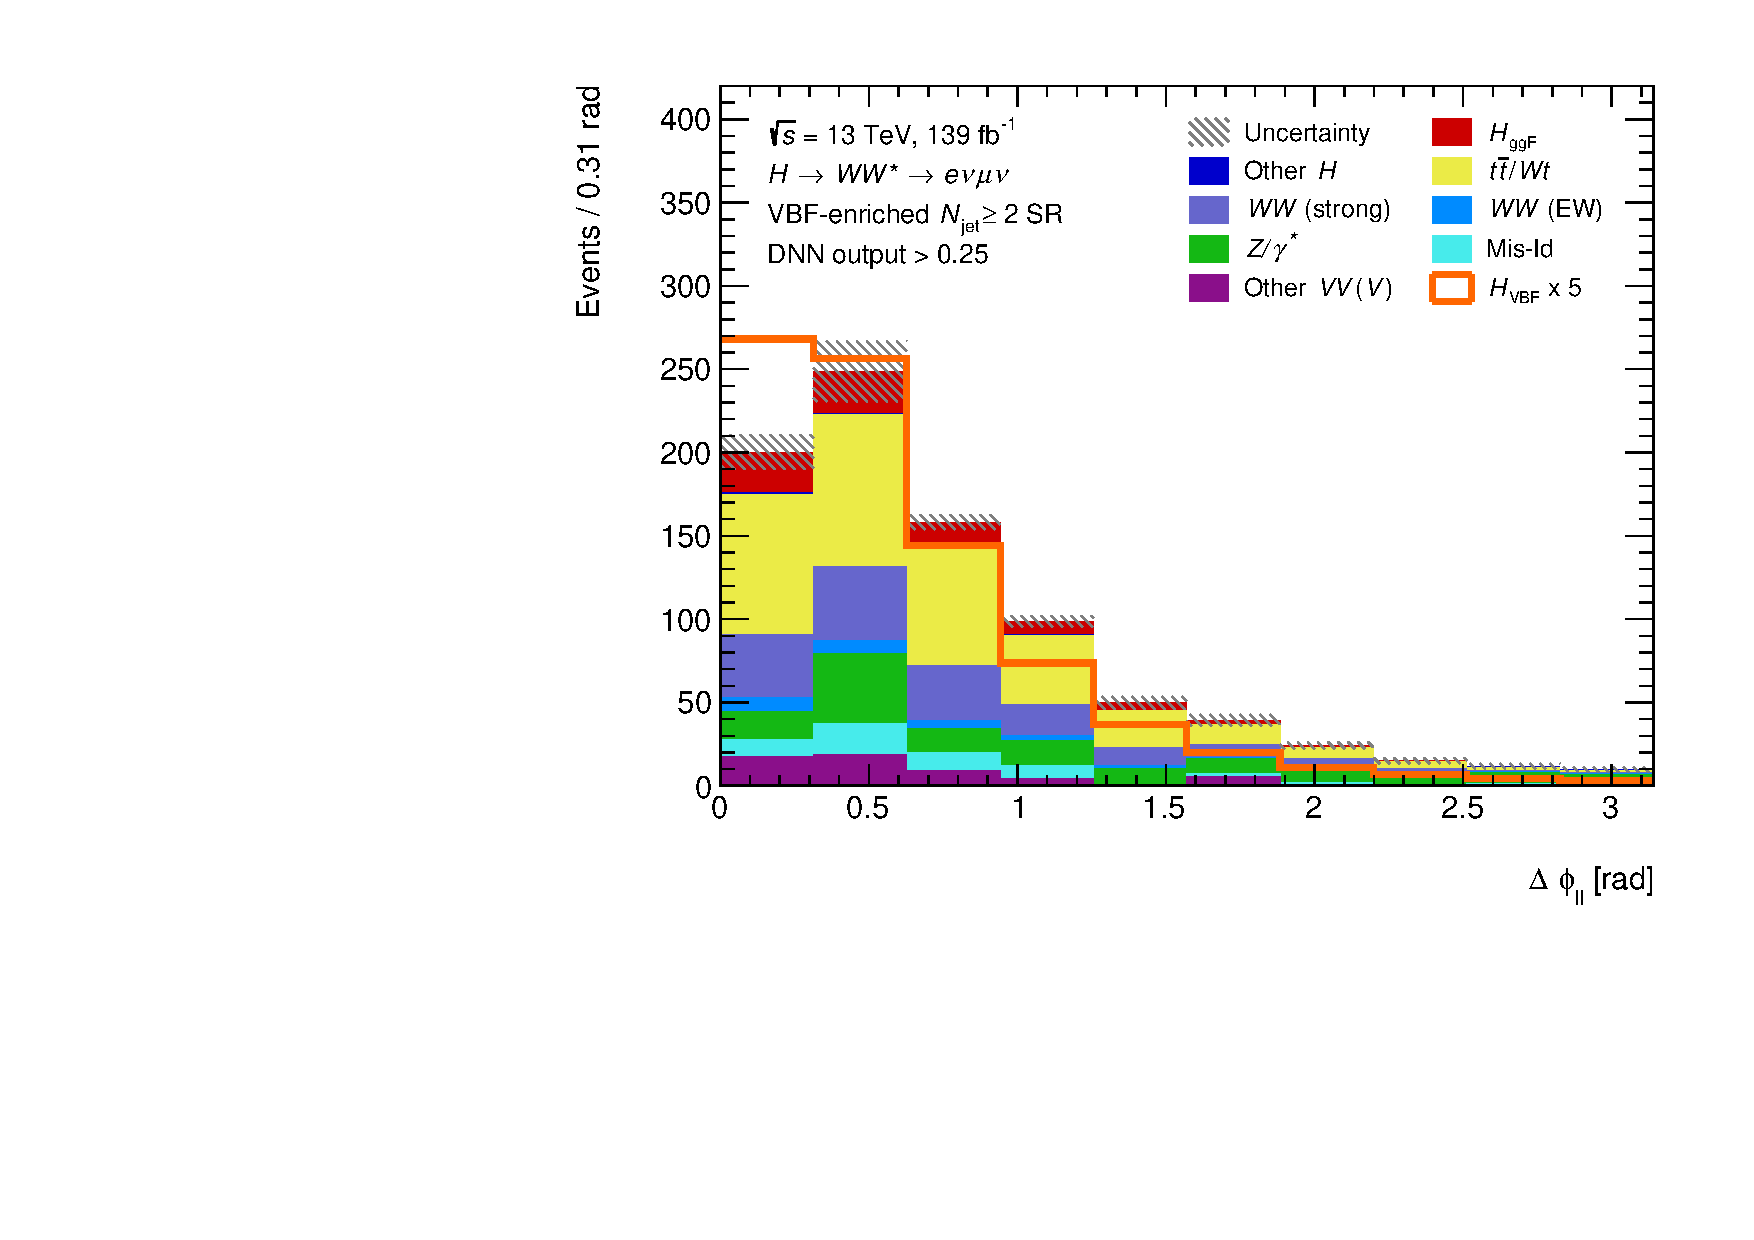
\includegraphics[width=0.32\textwidth]{figures/hww/dnn/blinded/run2-emme-CutVBFSR_DNN25-DPhill-lin.pdf} \hfill
        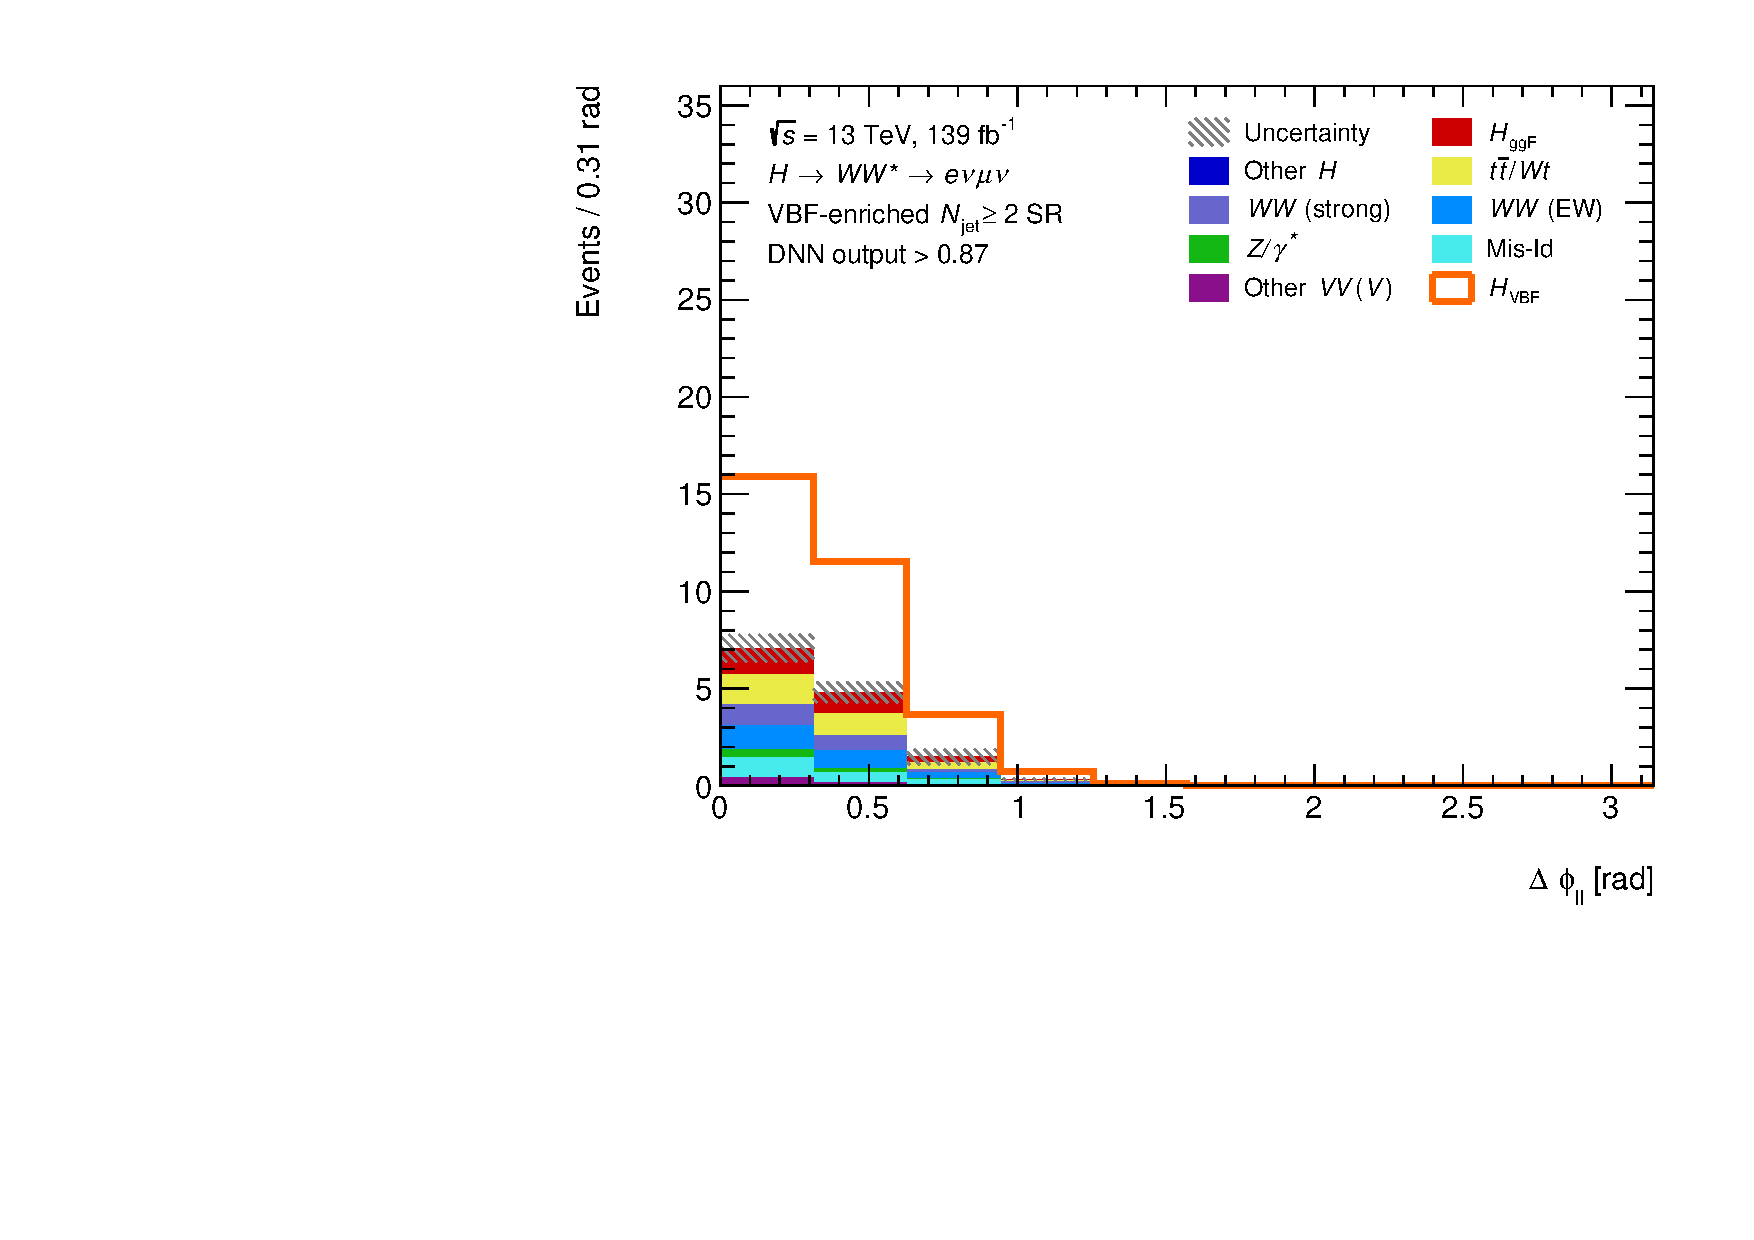
\includegraphics[width=0.32\textwidth]{figures/hww/dnn/blinded/run2-emme-CutVBFSR_DNN87-DPhill-lin.pdf}
    } \\
    \subfloat[$\mll$]{
        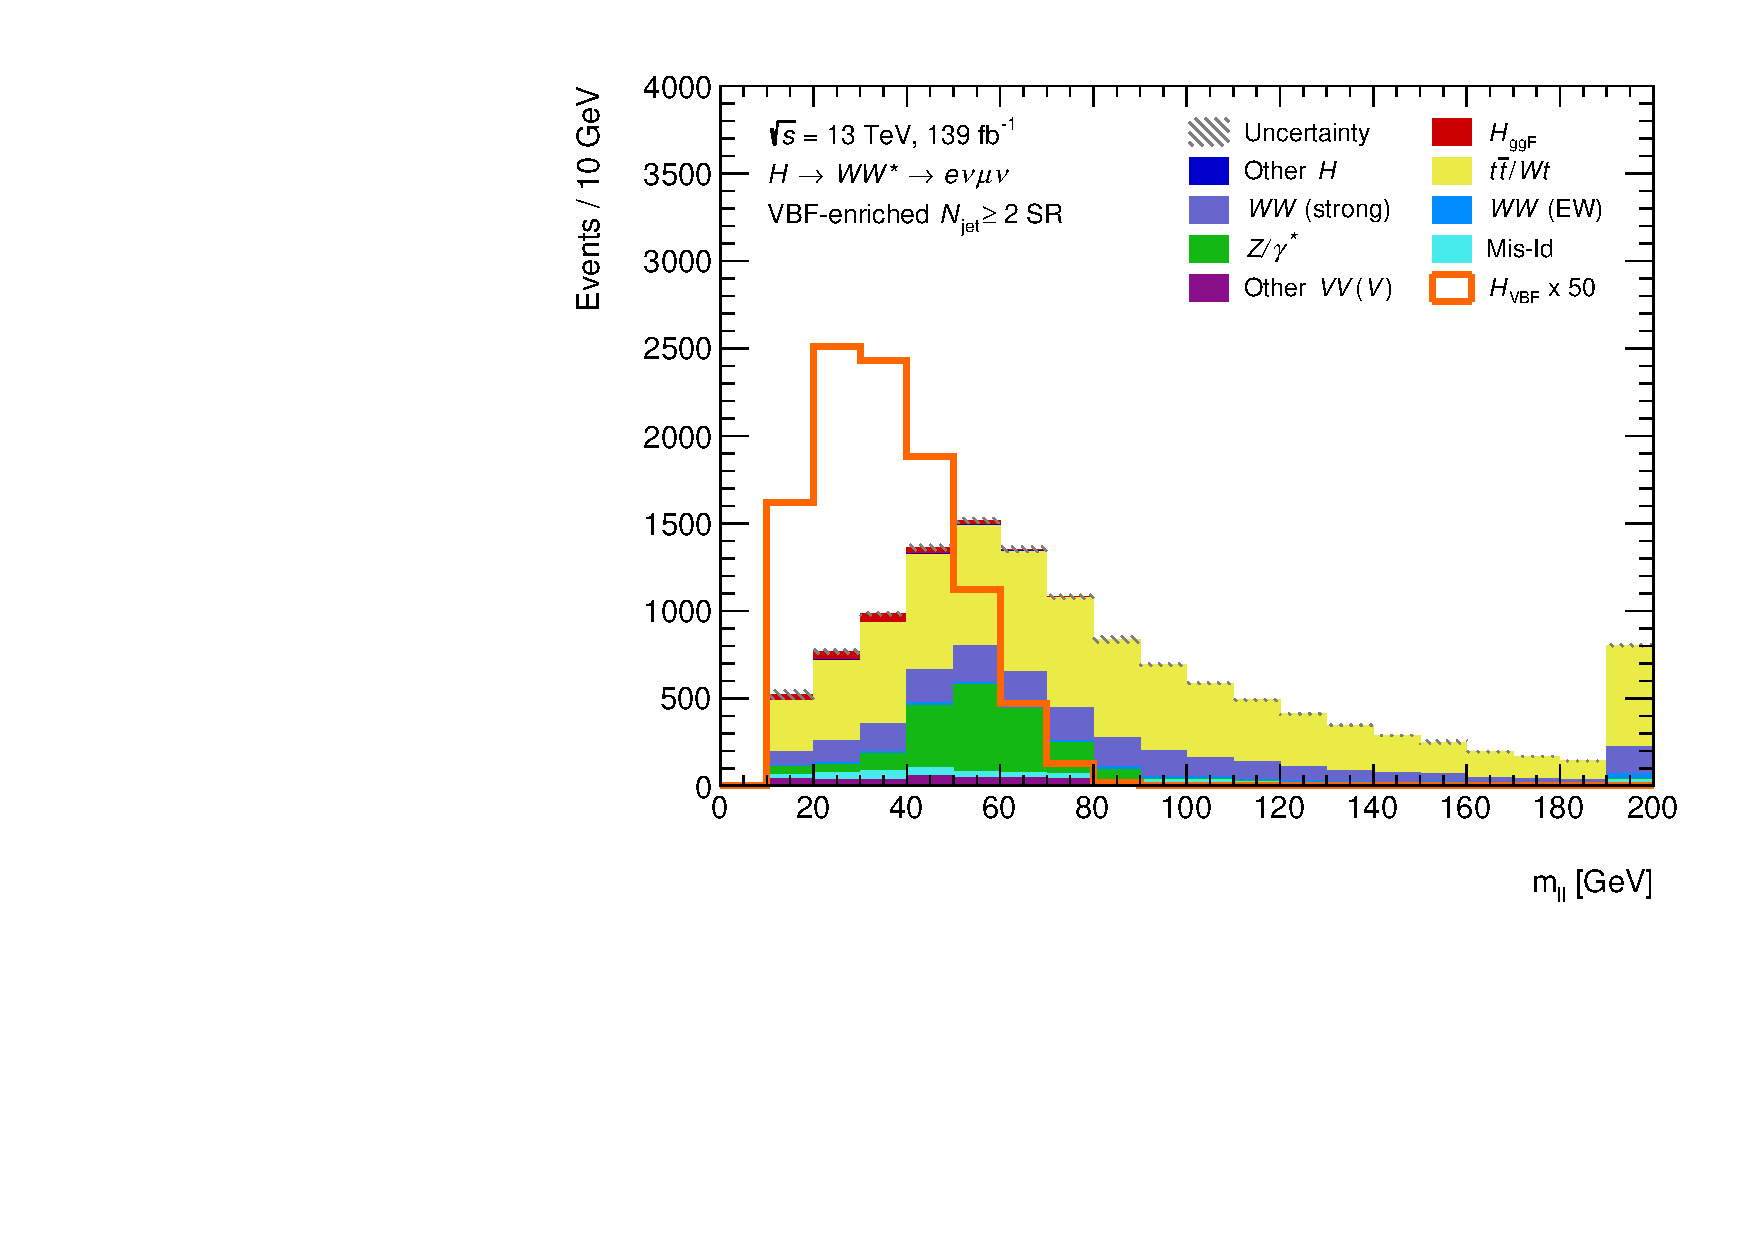
\includegraphics[width=0.32\textwidth]{figures/hww/dnn/blinded/run2-emme-CutVBF_SR-Mll-lin.pdf}
        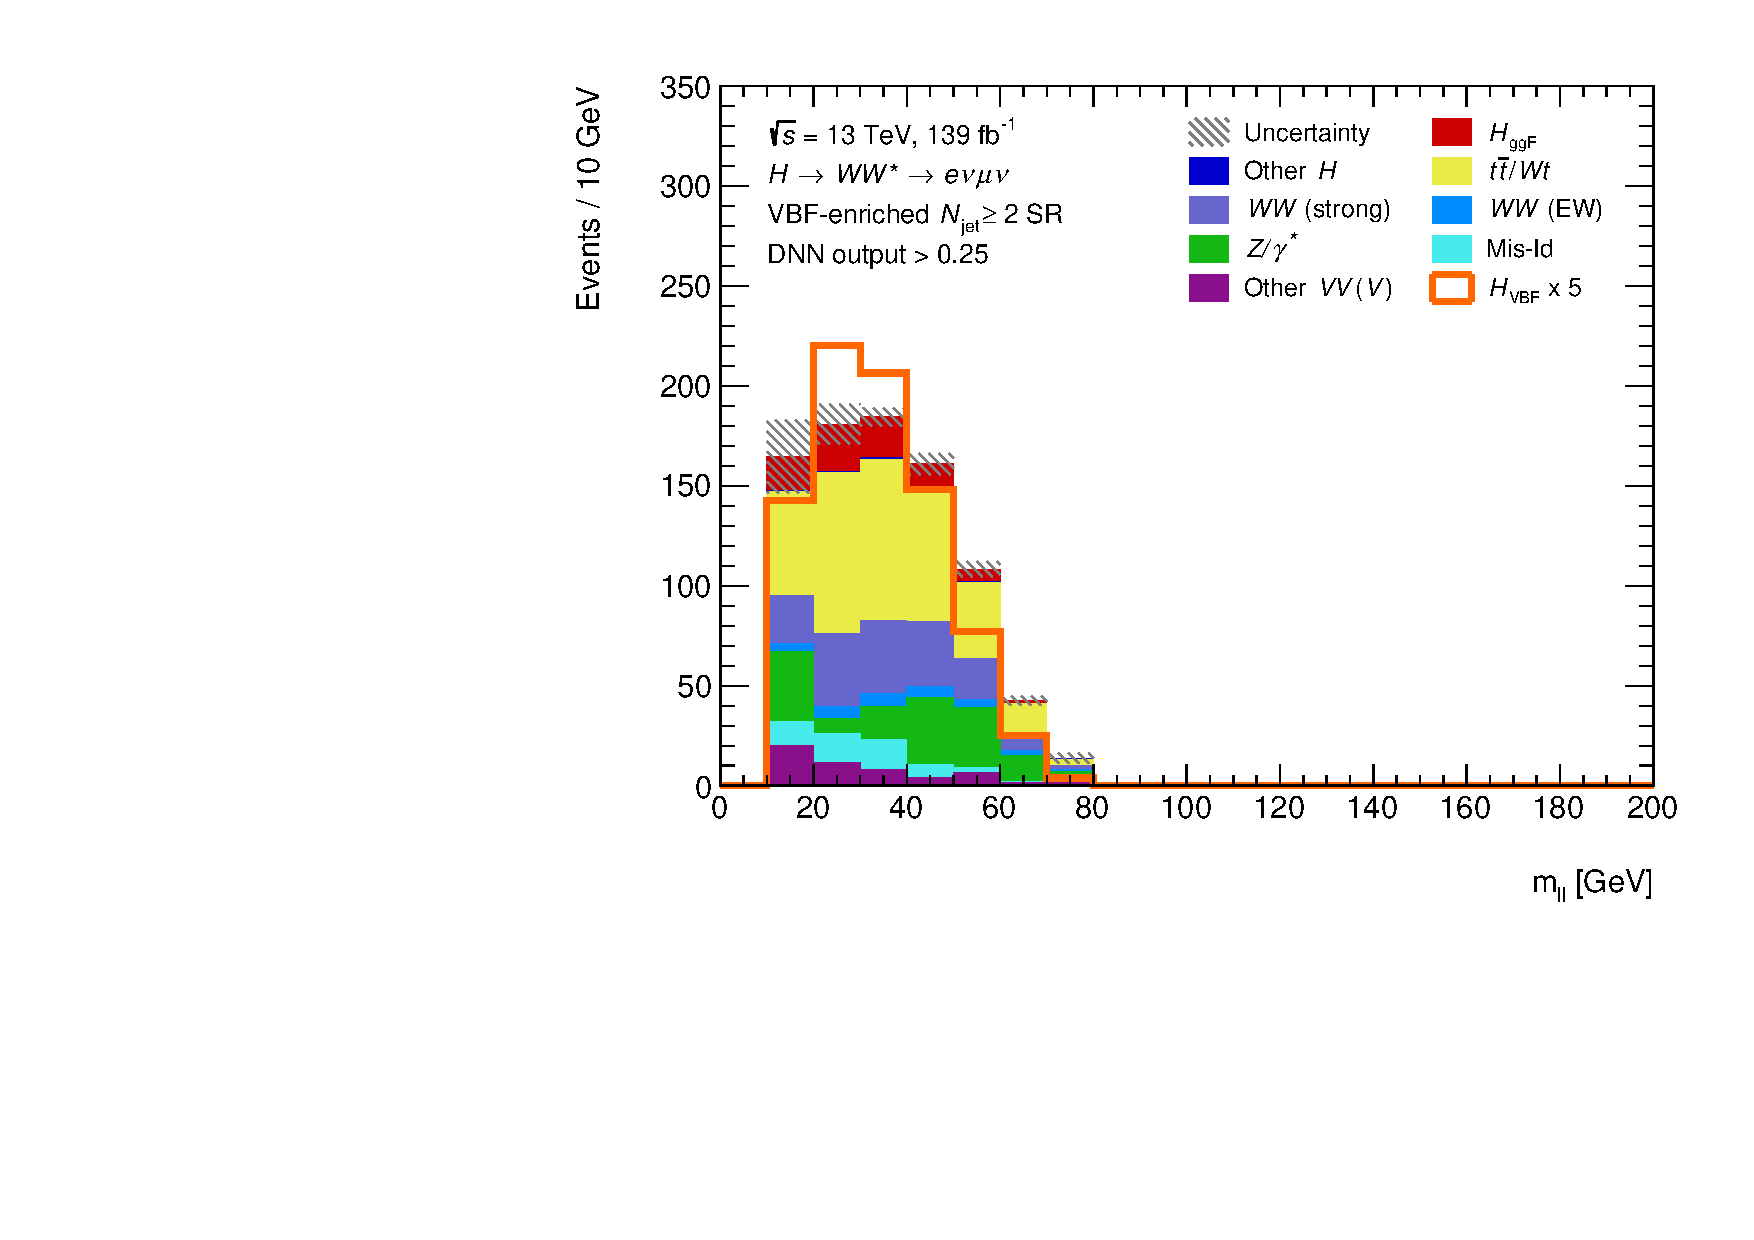
\includegraphics[width=0.32\textwidth]{figures/hww/dnn/blinded/run2-emme-CutVBFSR_DNN25-Mll-lin.pdf}
        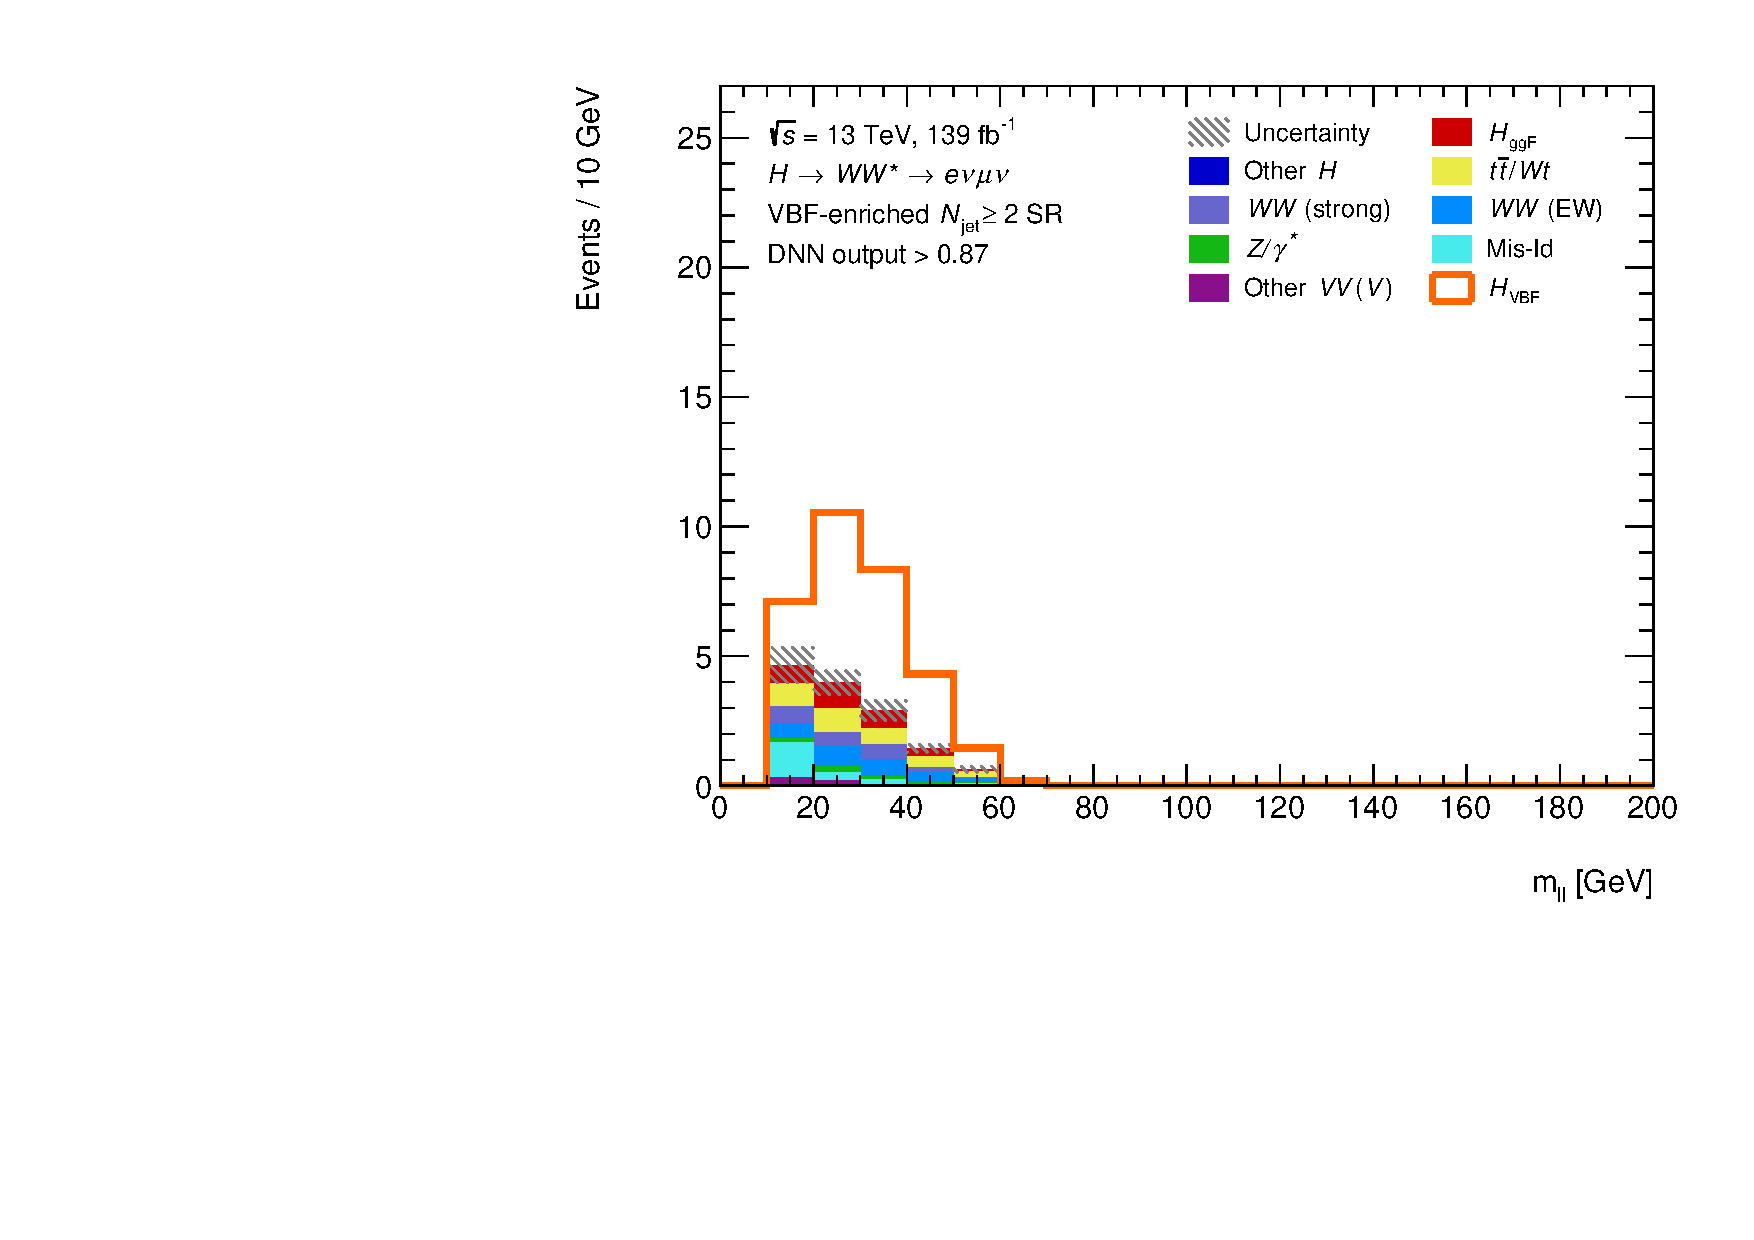
\includegraphics[width=0.32\textwidth]{figures/hww/dnn/blinded/run2-emme-CutVBFSR_DNN87-Mll-lin.pdf}
    } \\
    \subfloat[$\mT$]{
        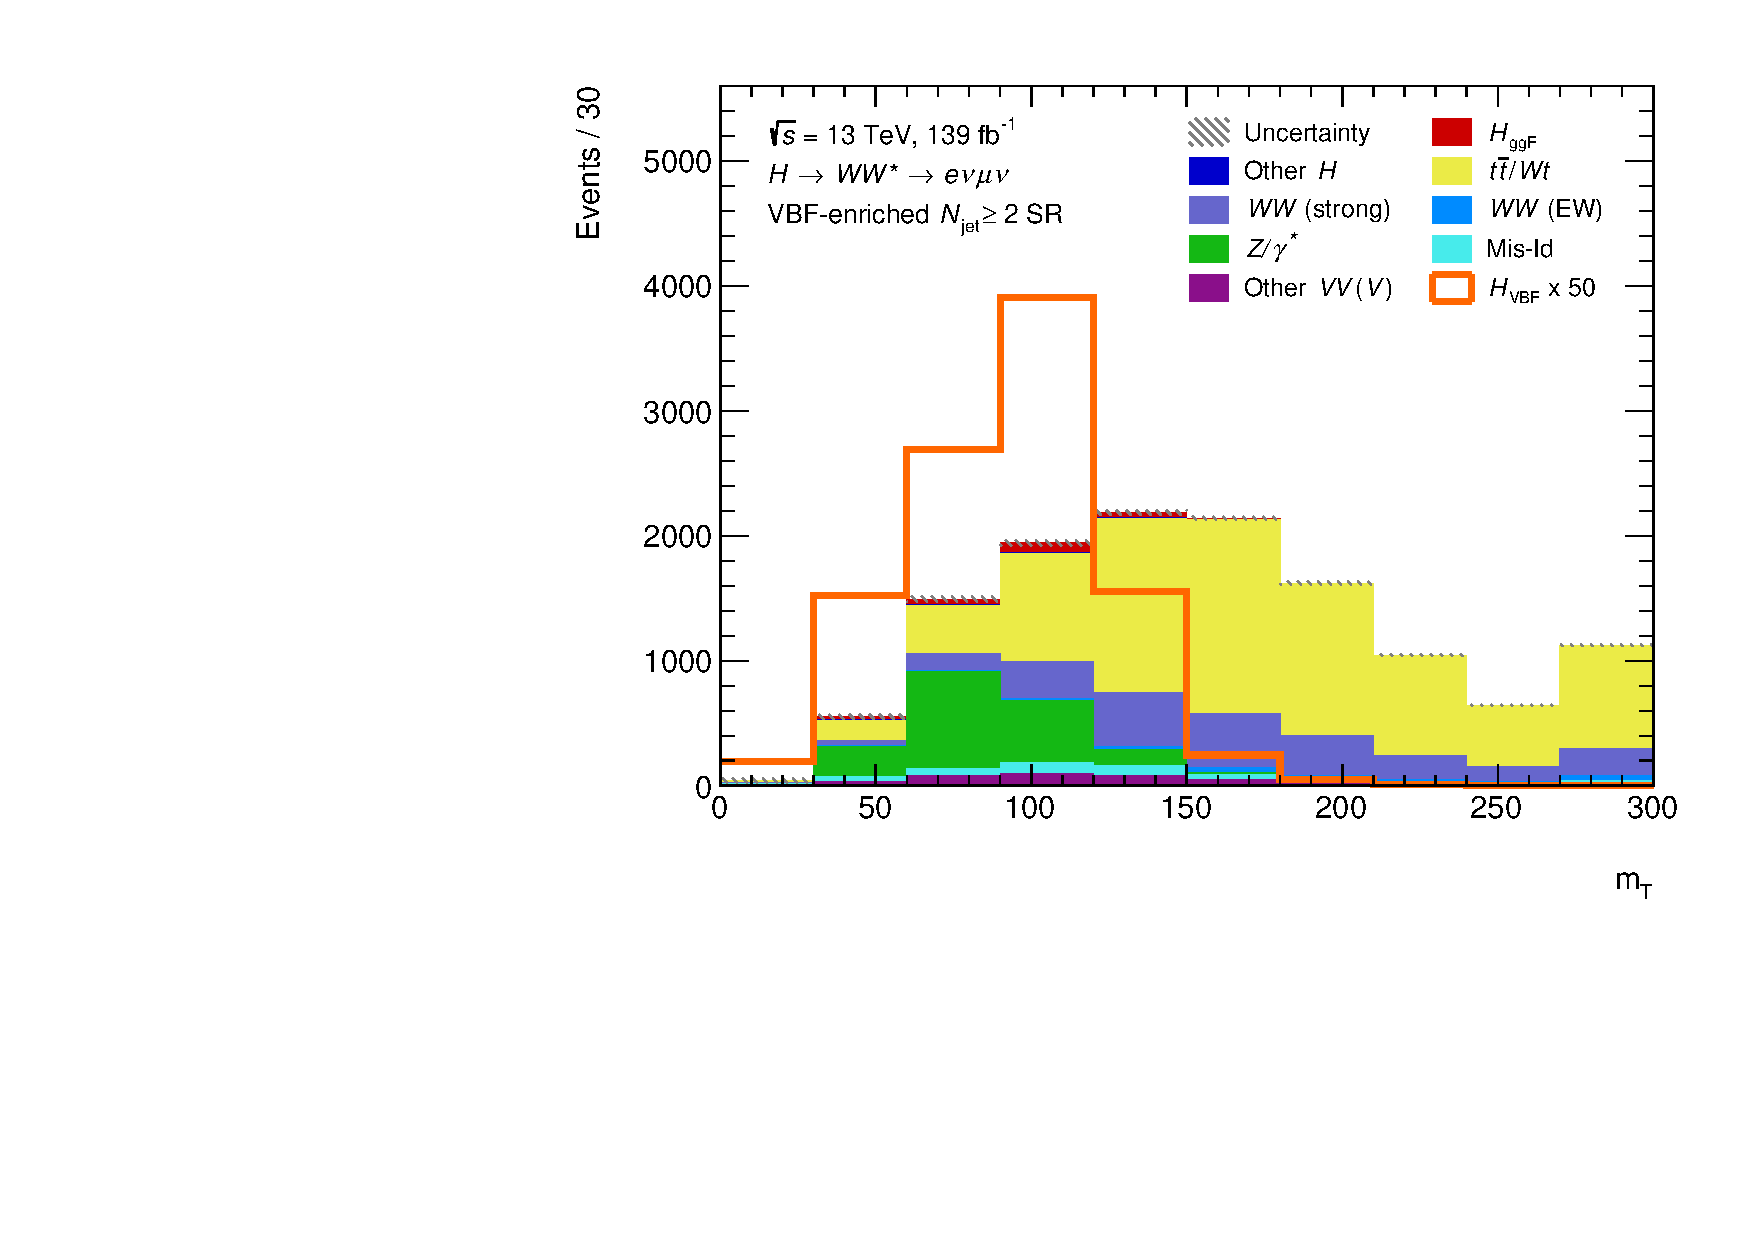
\includegraphics[width=0.32\textwidth]{figures/hww/dnn/blinded/run2-emme-CutVBF_SR-MT-lin.pdf} \hfill
        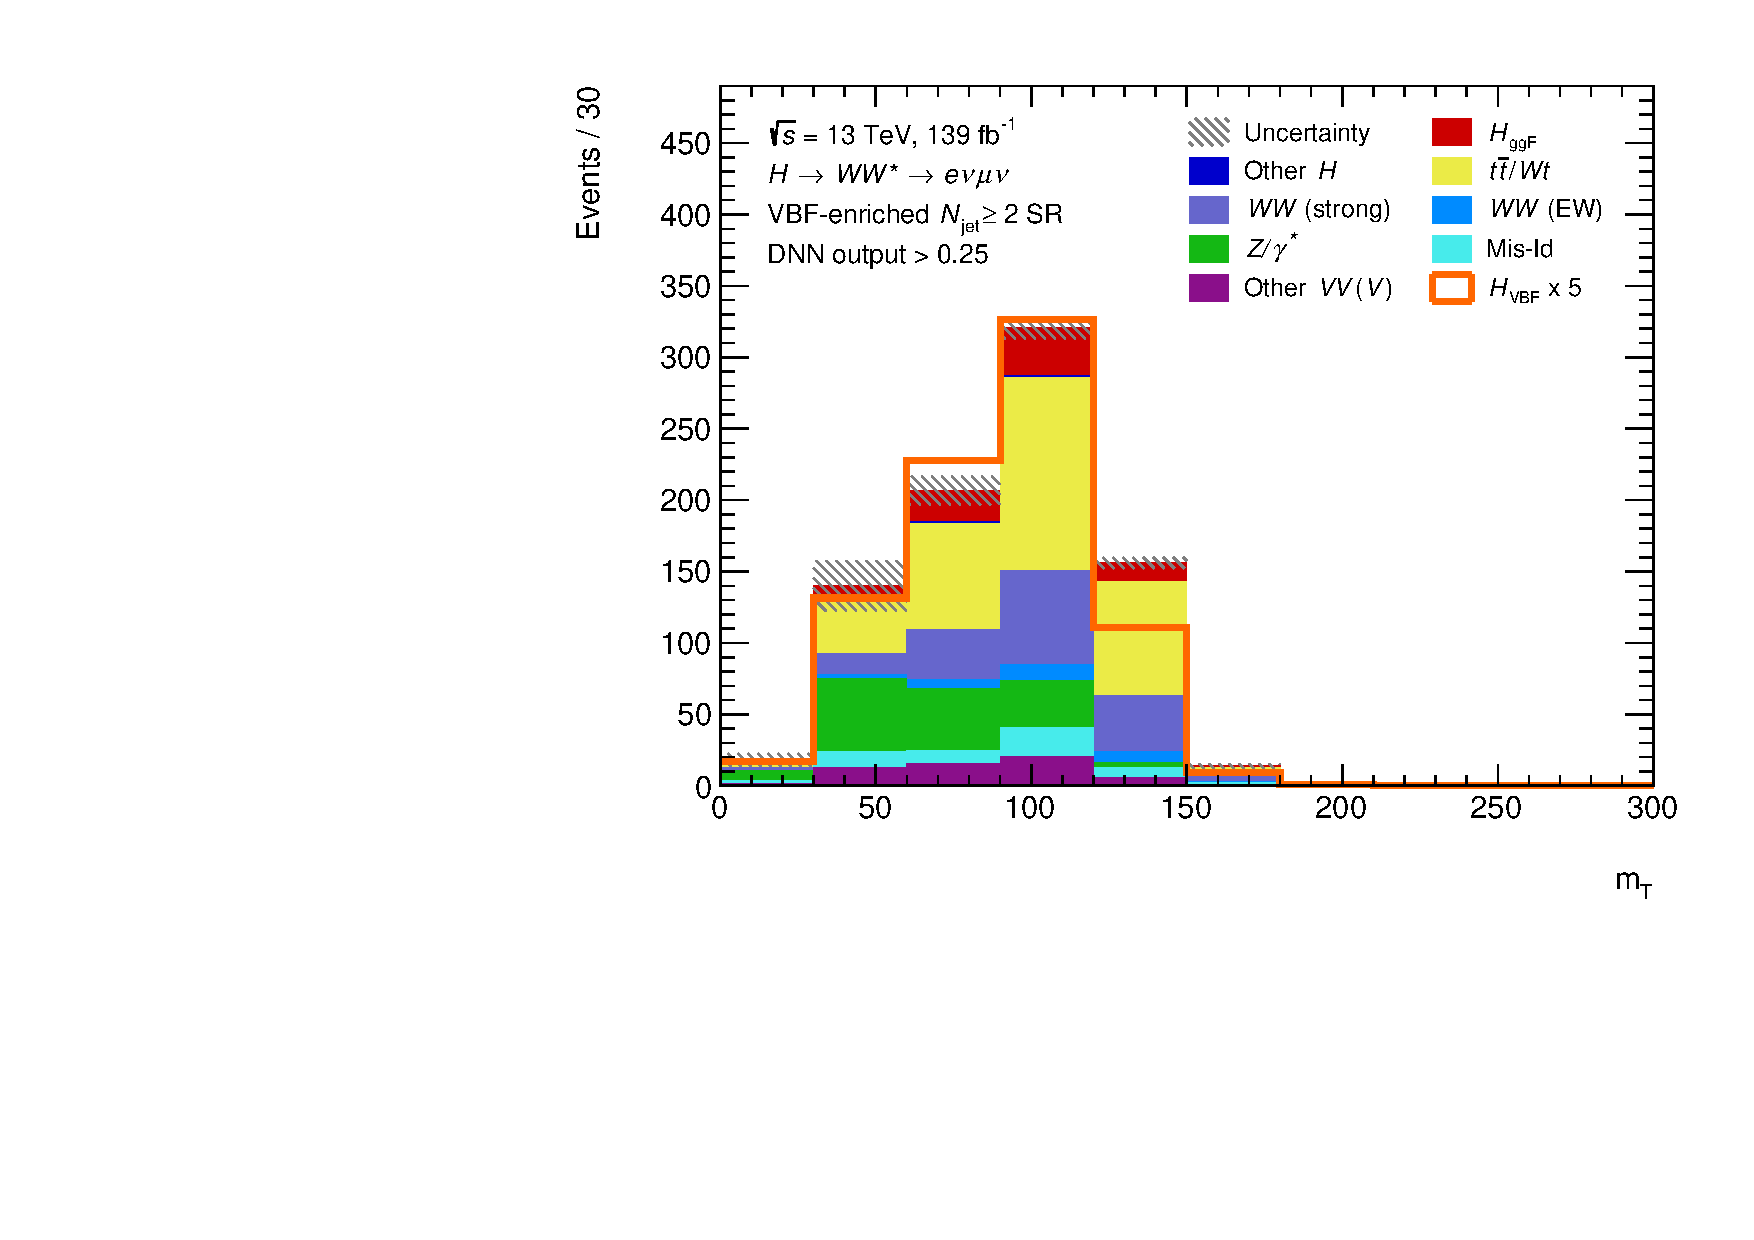
\includegraphics[width=0.32\textwidth]{figures/hww/dnn/blinded/run2-emme-CutVBFSR_DNN25-MT-lin.pdf} \hfill
        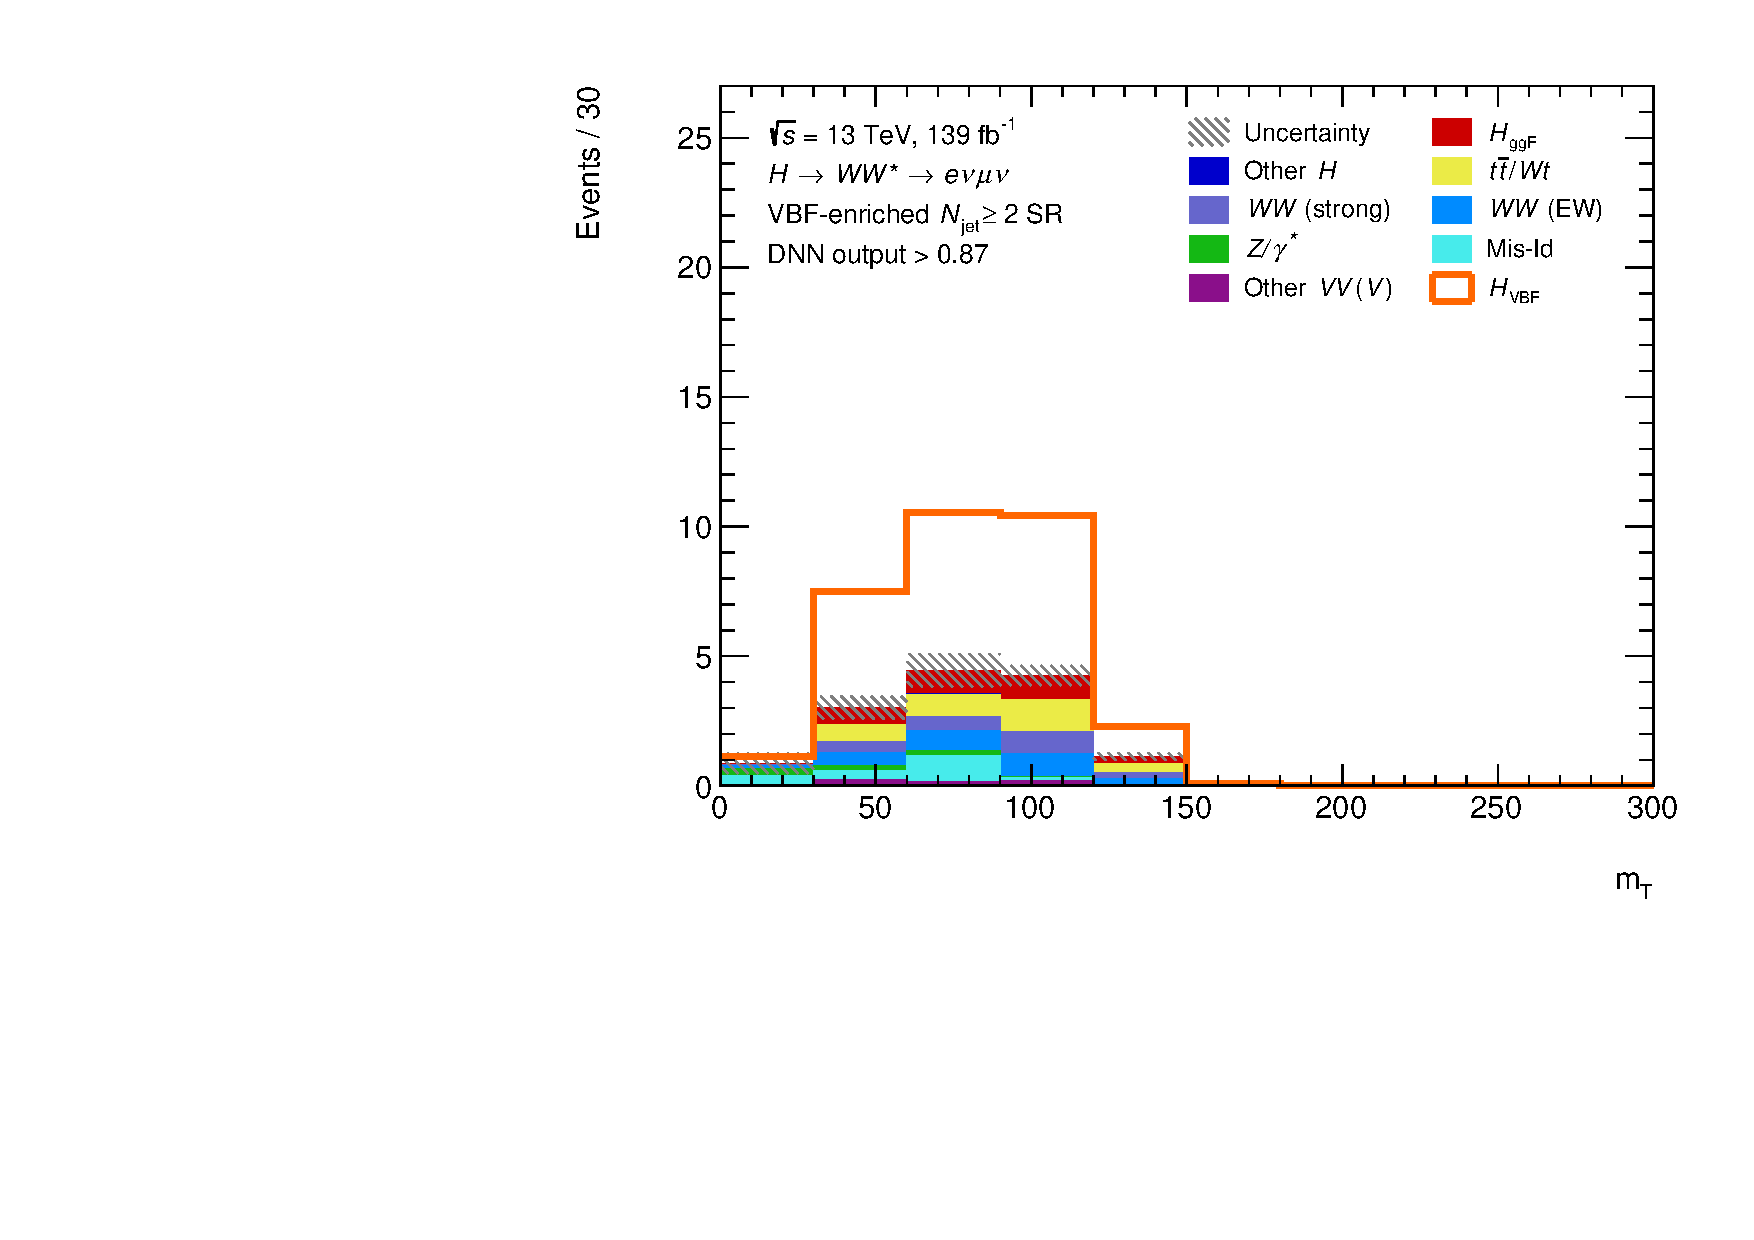
\includegraphics[width=0.32\textwidth]{figures/hww/dnn/blinded/run2-emme-CutVBFSR_DNN87-MT-lin.pdf}
    } 
    {\caption{Distributions of $\dphill$, $\mll$, $\mT$ in the VBF signal region.
        Each row corresponds to one variable with different selections made on the DNN output.
        \label{fig:dnn-inputs-hwwdecay} }}
\end{figure}



\begin{figure}[h]
    \centering
    \subfloat[$\pttot$]{
        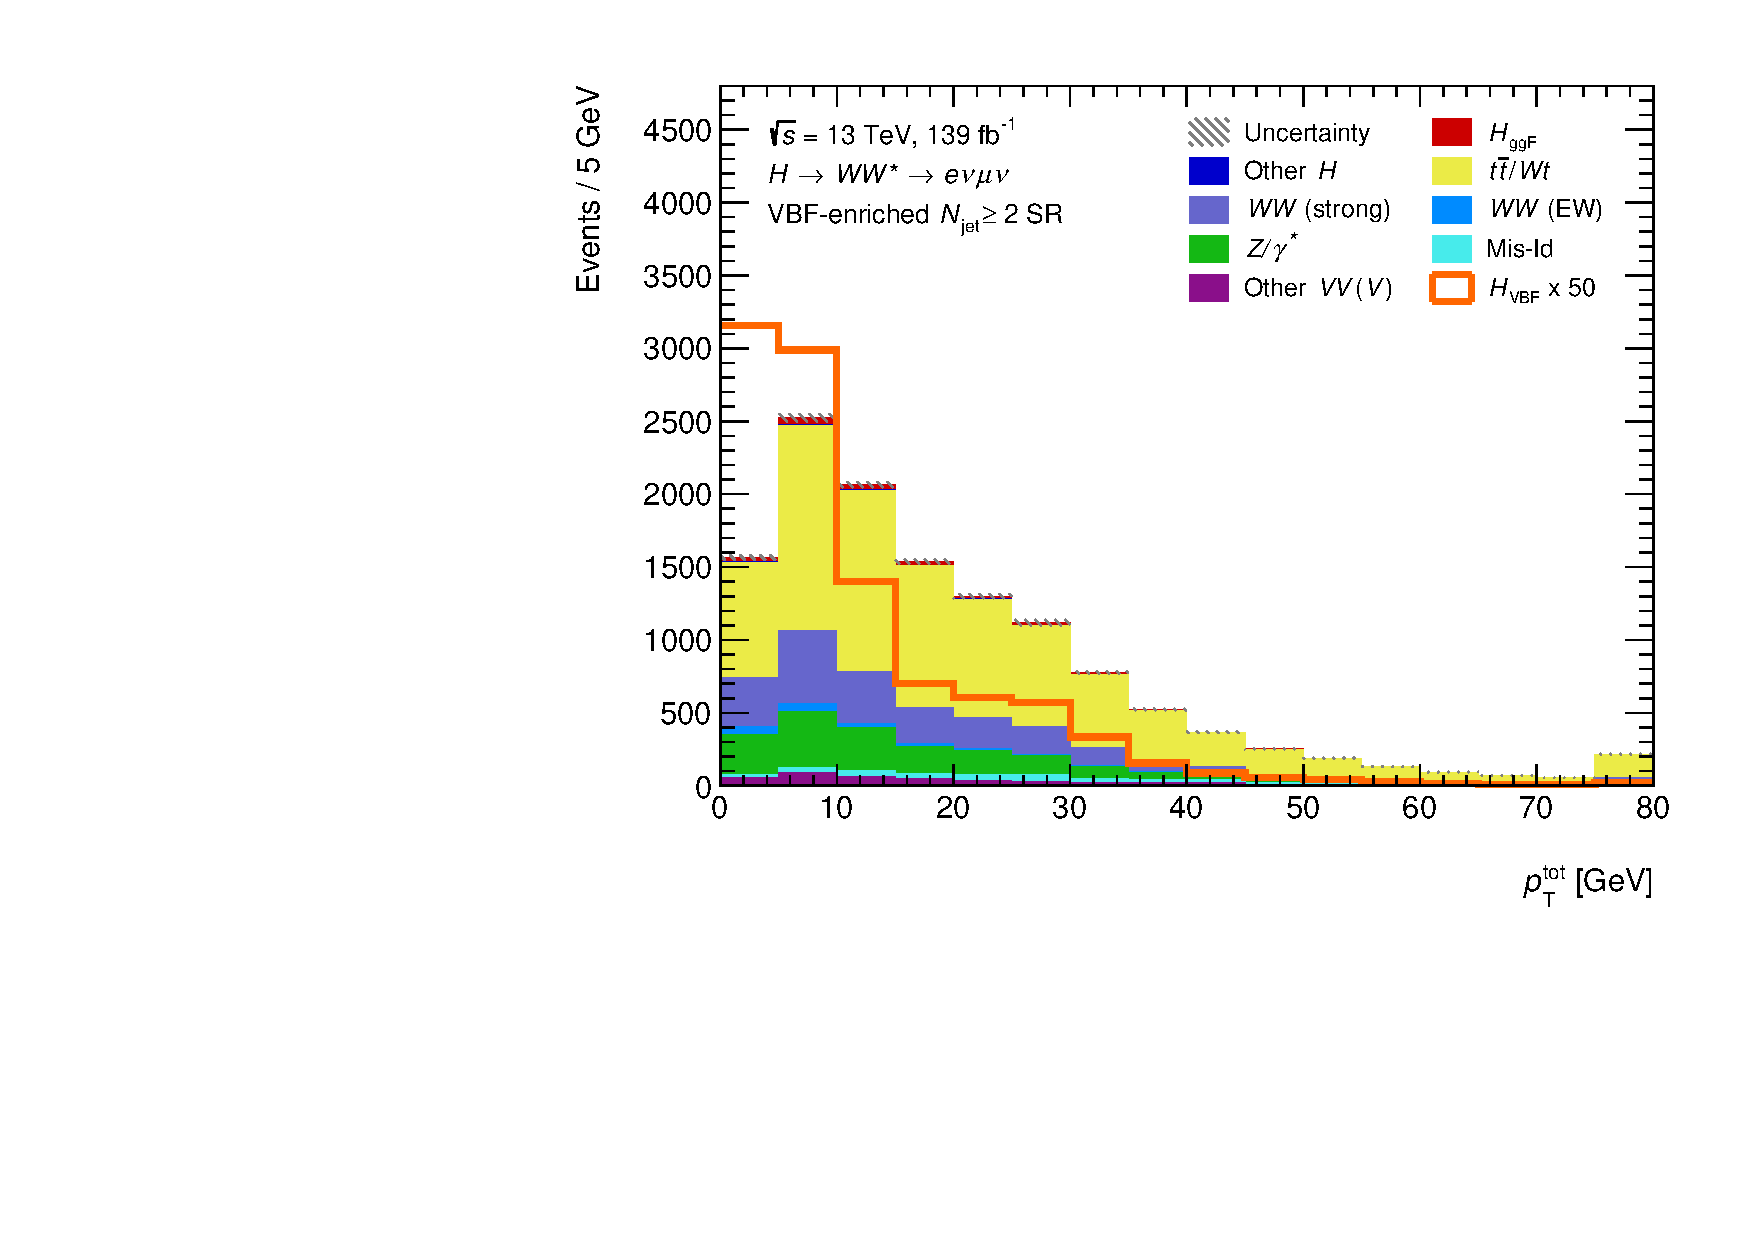
\includegraphics[width=0.32\textwidth]{figures/hww/dnn/blinded/run2-emme-CutVBF_SR-PtTot-lin.pdf} \hfill
        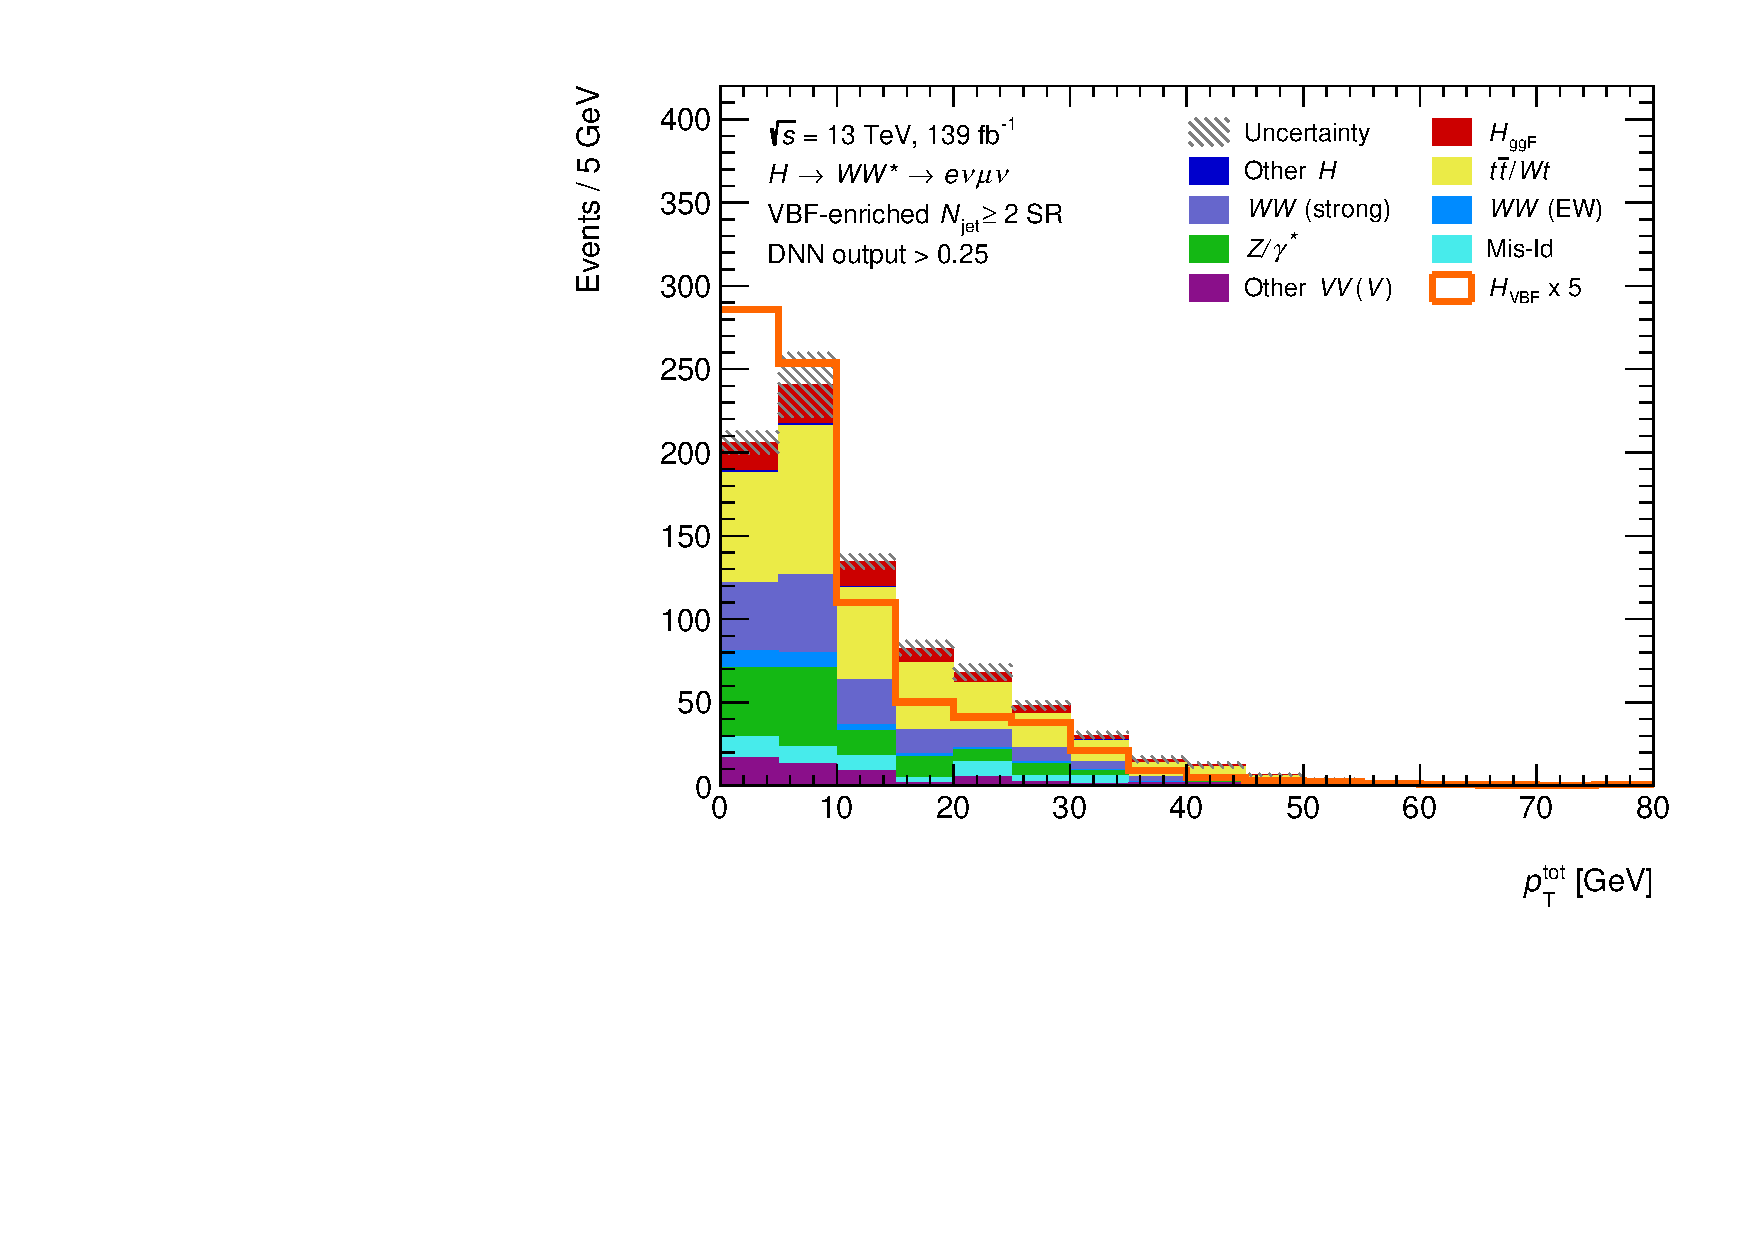
\includegraphics[width=0.32\textwidth]{figures/hww/dnn/blinded/run2-emme-CutVBFSR_DNN25-PtTot-lin.pdf} \hfill
        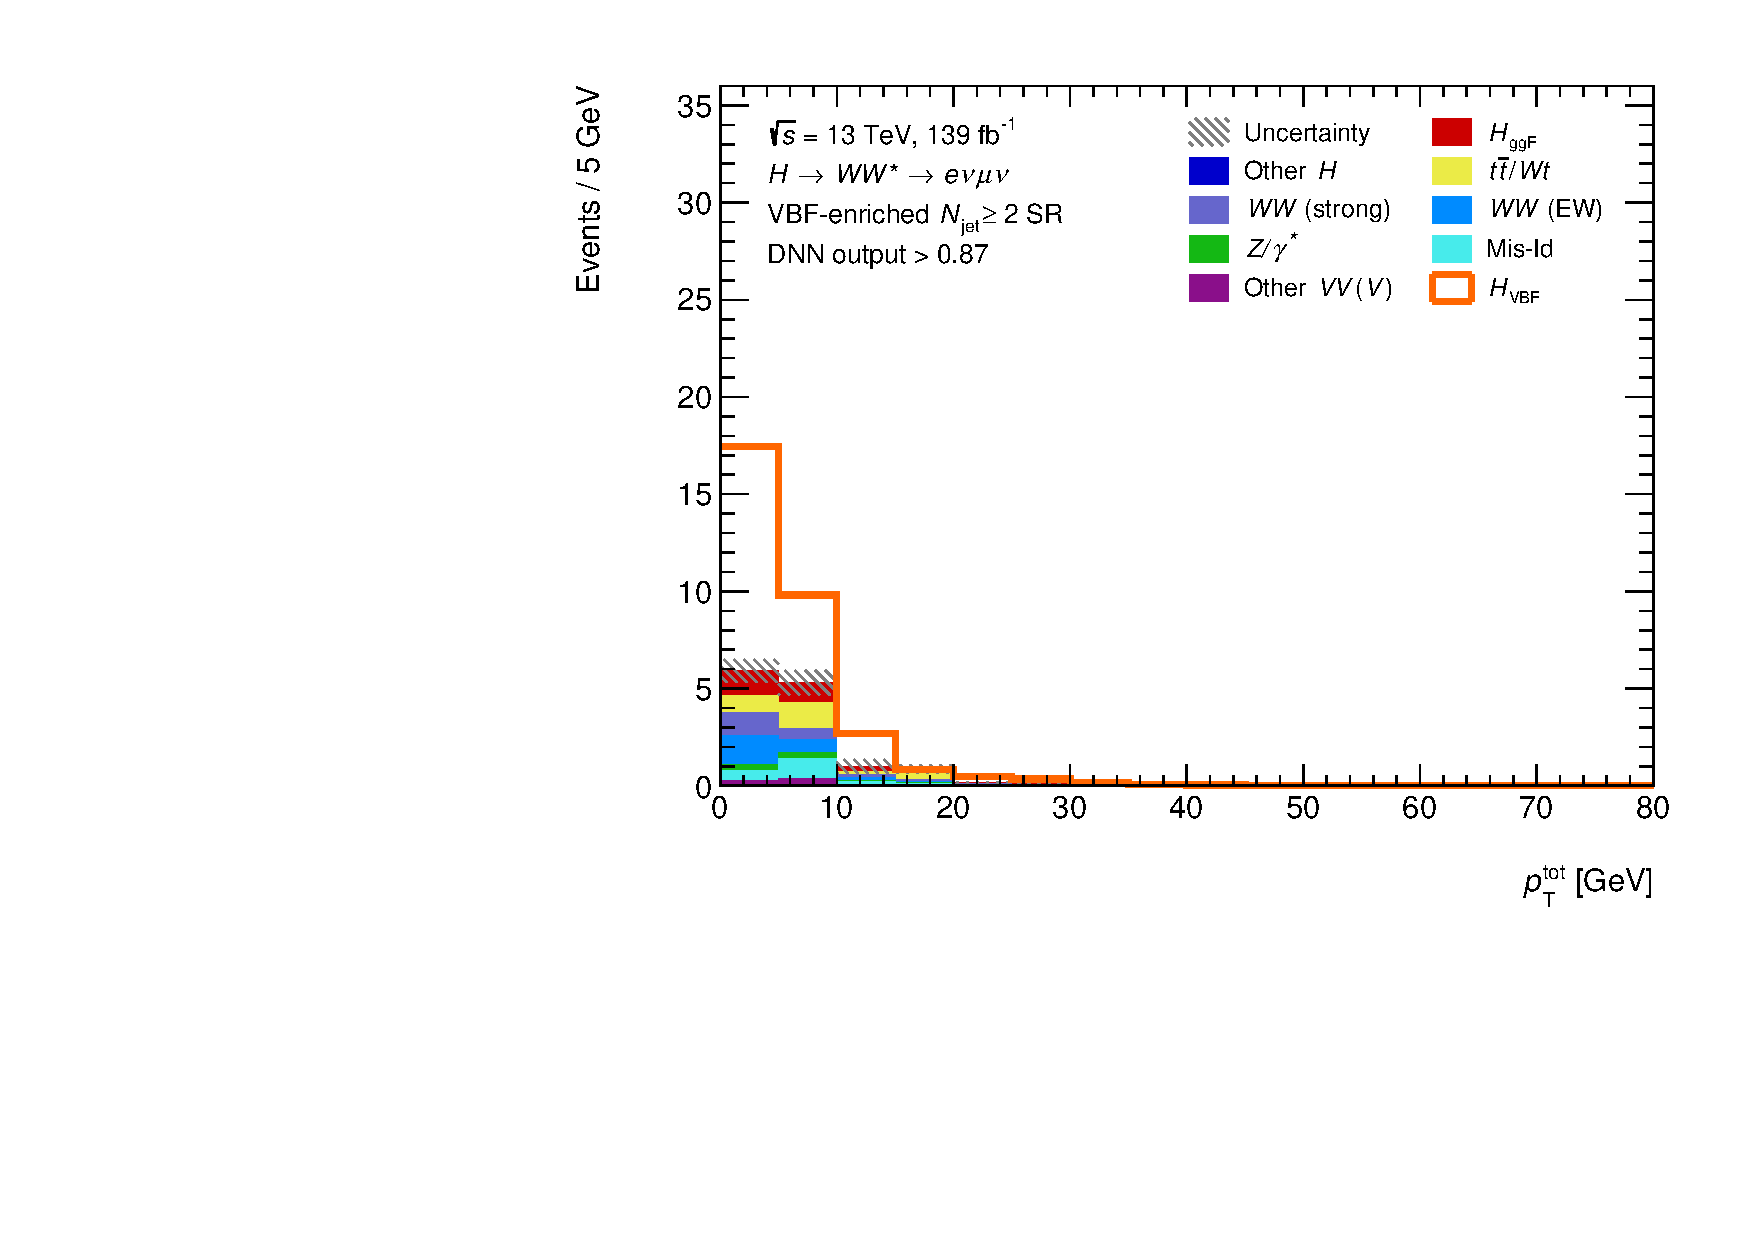
\includegraphics[width=0.32\textwidth]{figures/hww/dnn/blinded/run2-emme-CutVBFSR_DNN87-PtTot-lin.pdf}
    } \\
    \subfloat[$\METSig$]{
        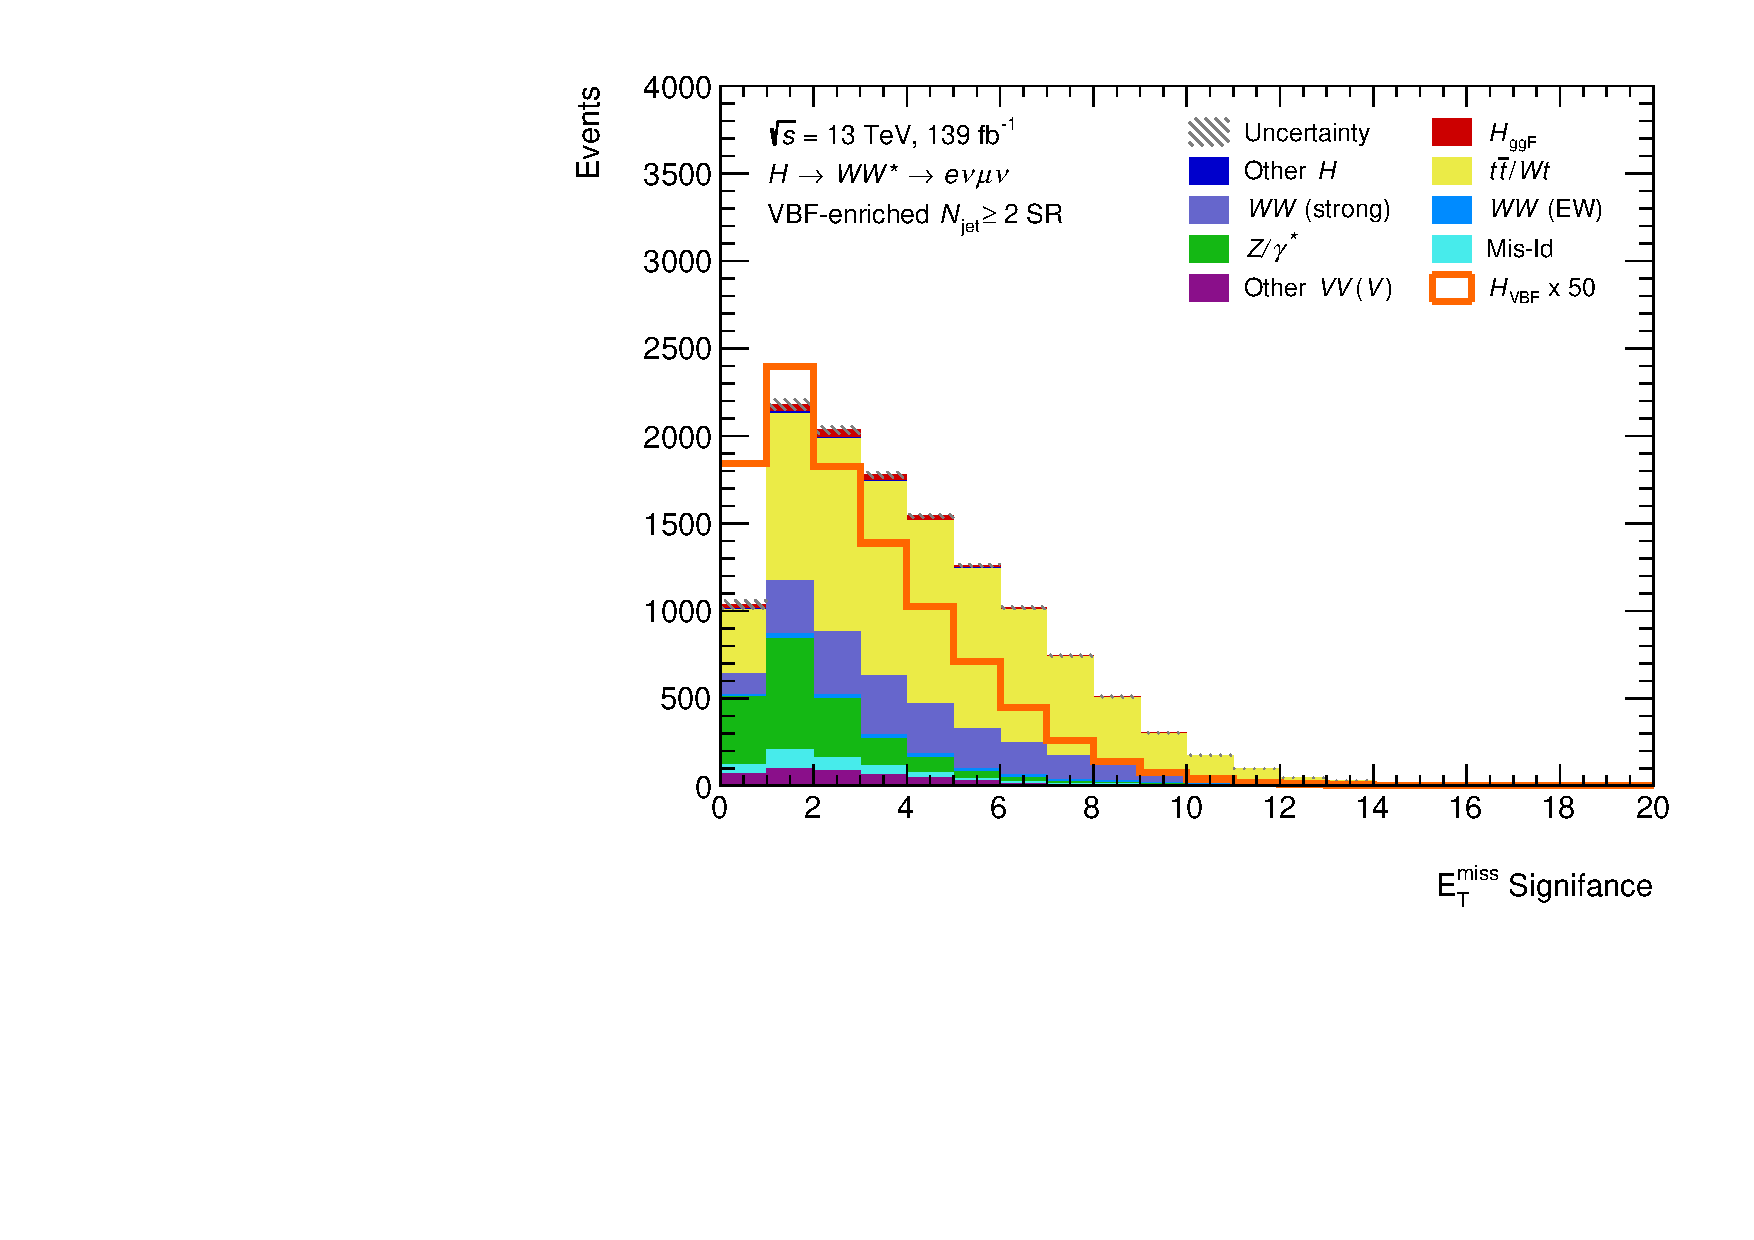
\includegraphics[width=0.32\textwidth]{figures/hww/dnn/blinded/run2-emme-CutVBF_SR-METSig_broad-lin.pdf} \hfill
        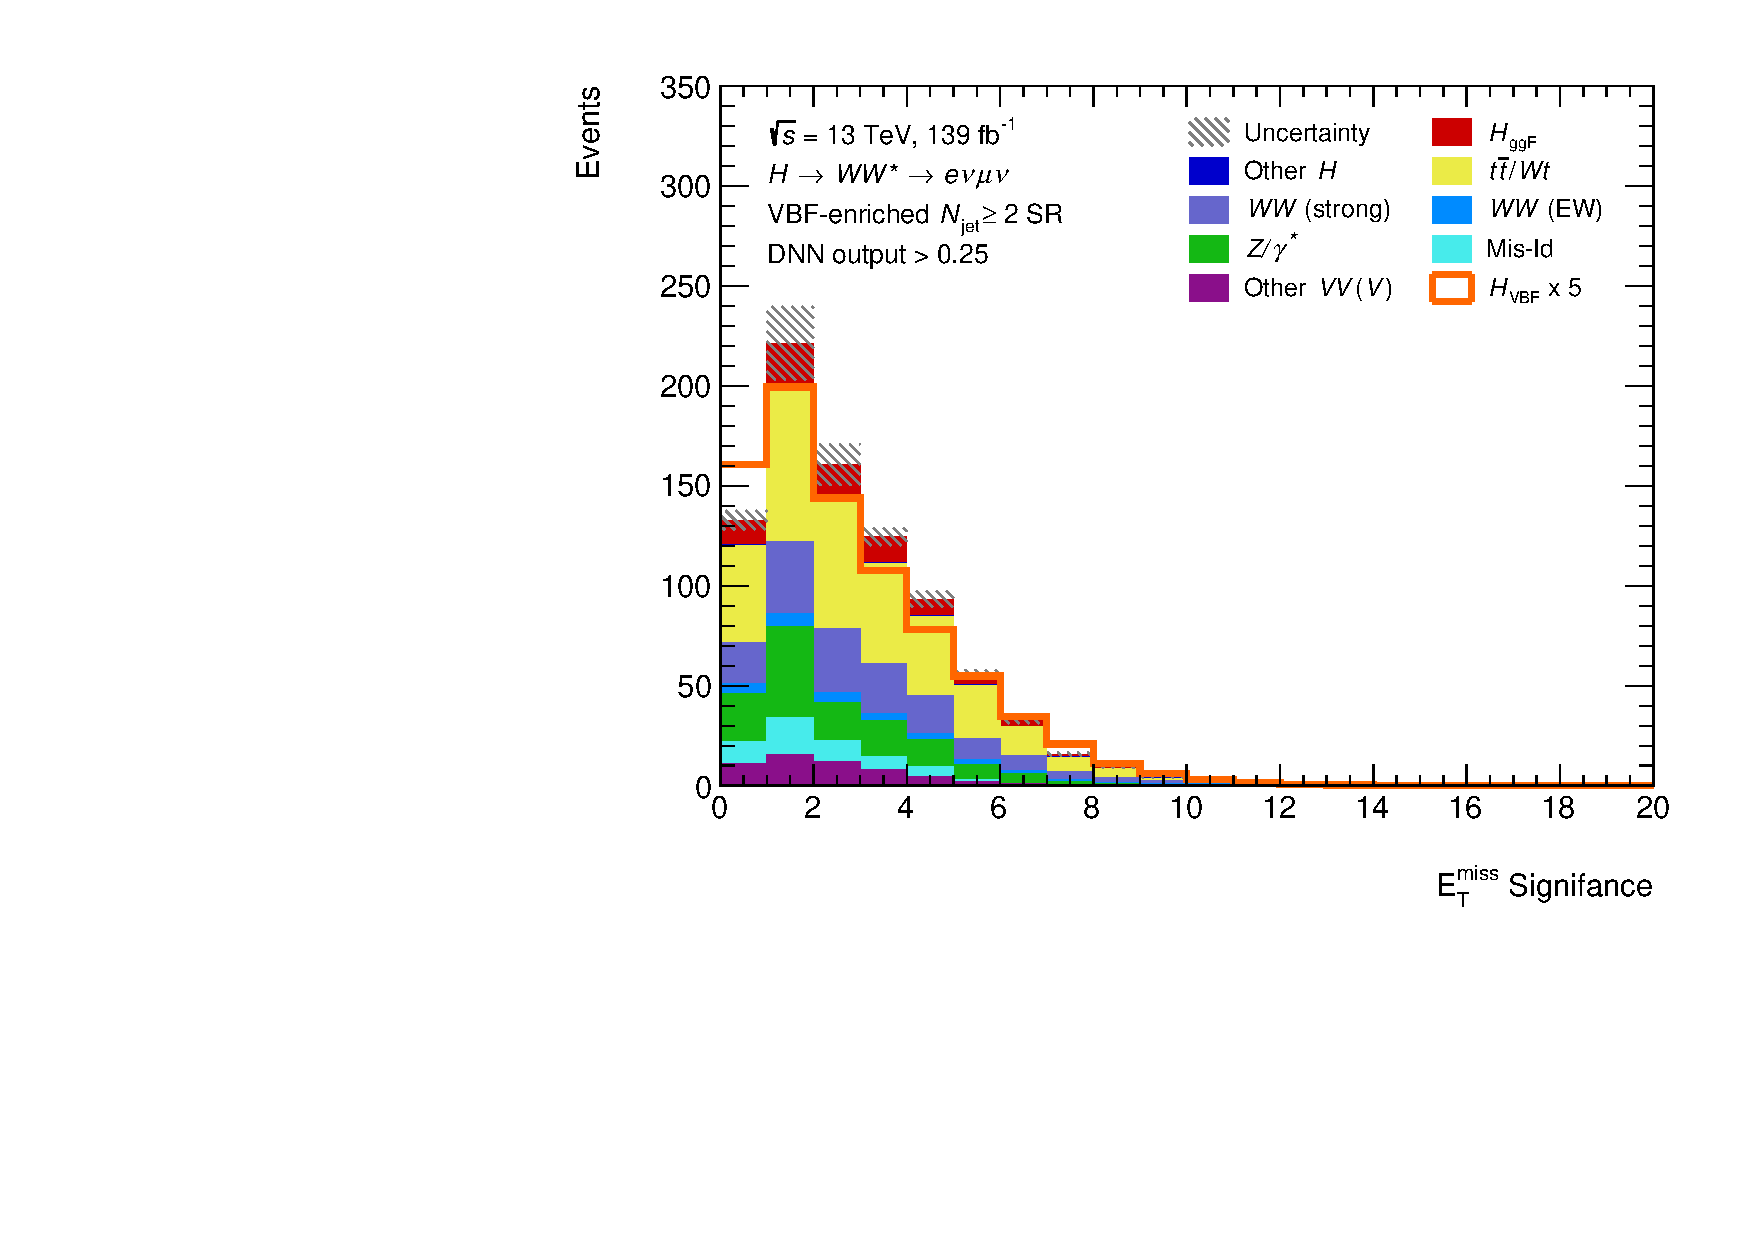
\includegraphics[width=0.32\textwidth]{figures/hww/dnn/blinded/run2-emme-CutVBFSR_DNN25-METSig_broad-lin.pdf} \hfill
        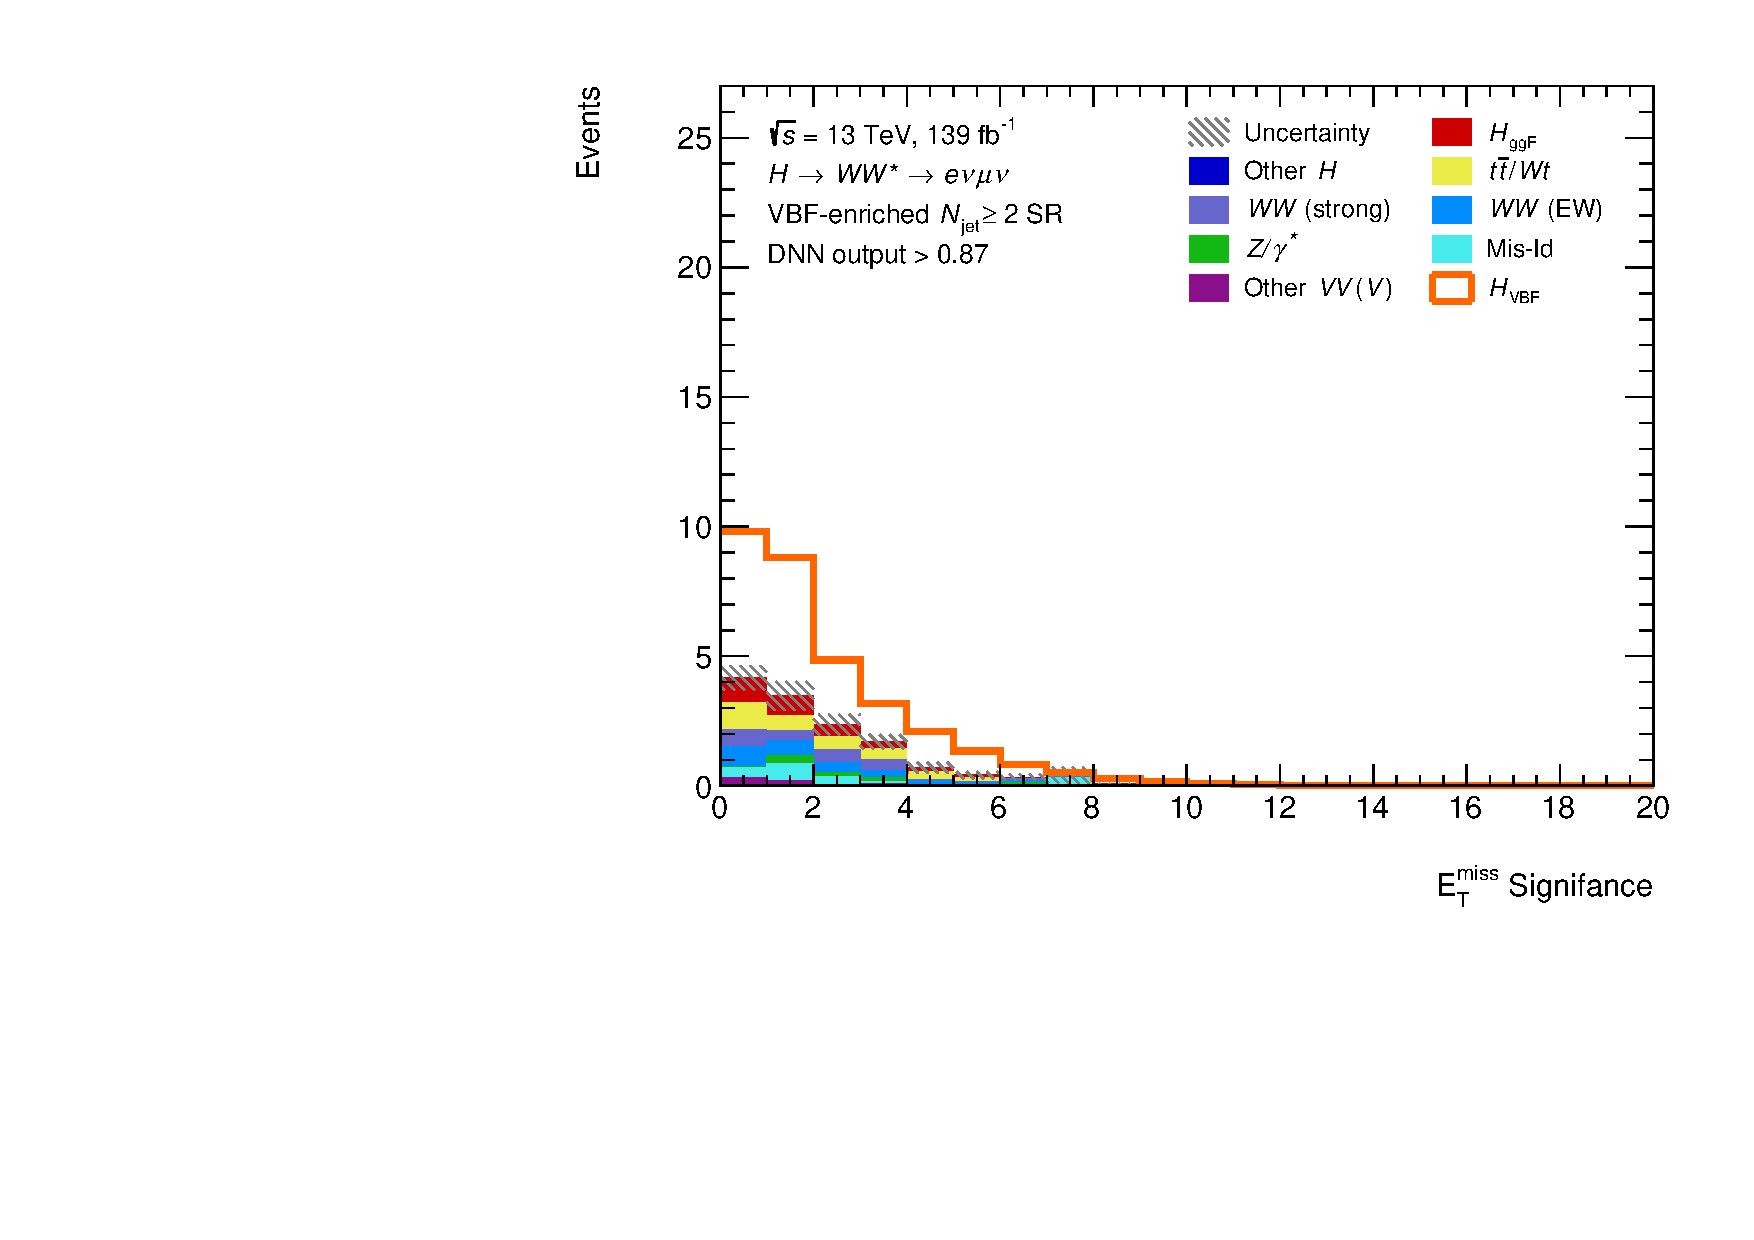
\includegraphics[width=0.32\textwidth]{figures/hww/dnn/blinded/run2-emme-CutVBFSR_DNN87-METSig_broad-lin.pdf}
    } \\
    {\caption{Distributions of $\pttot$ and $\METSig$ in the VBF signal region.
            Each row shows one variable with different cuts on the DNN output distribution being applied in different columns.
            \label{fig:dnn-inputs-top-sup} }}
\end{figure}




\FloatBarrier
\chapter{Auxiliary material for \HWW analysis}


\FloatBarrier
\section{Post-fit Distributions of the DNN input variables}
\label{app:post-fit-distributions}
\TDinote{}{MAYBE!?}


\FloatBarrier
\section{DNN distributions in STXS SRs}
\Cref{fig:dnn-output-vbf-stxs} shows the distribution of the DNN output in the top-quark and \Ztautau CRs used in the VBF, STXS analysis. 

\captionsetup[subfloat]{captionskip=5pt} % space between subfloat caption and image
\begin{figure}[t]
    \centering
    \subfloat[{\tiny $350 \leq \mjj < 700~\GeV, \pTH < 200~\GeV$}]{
        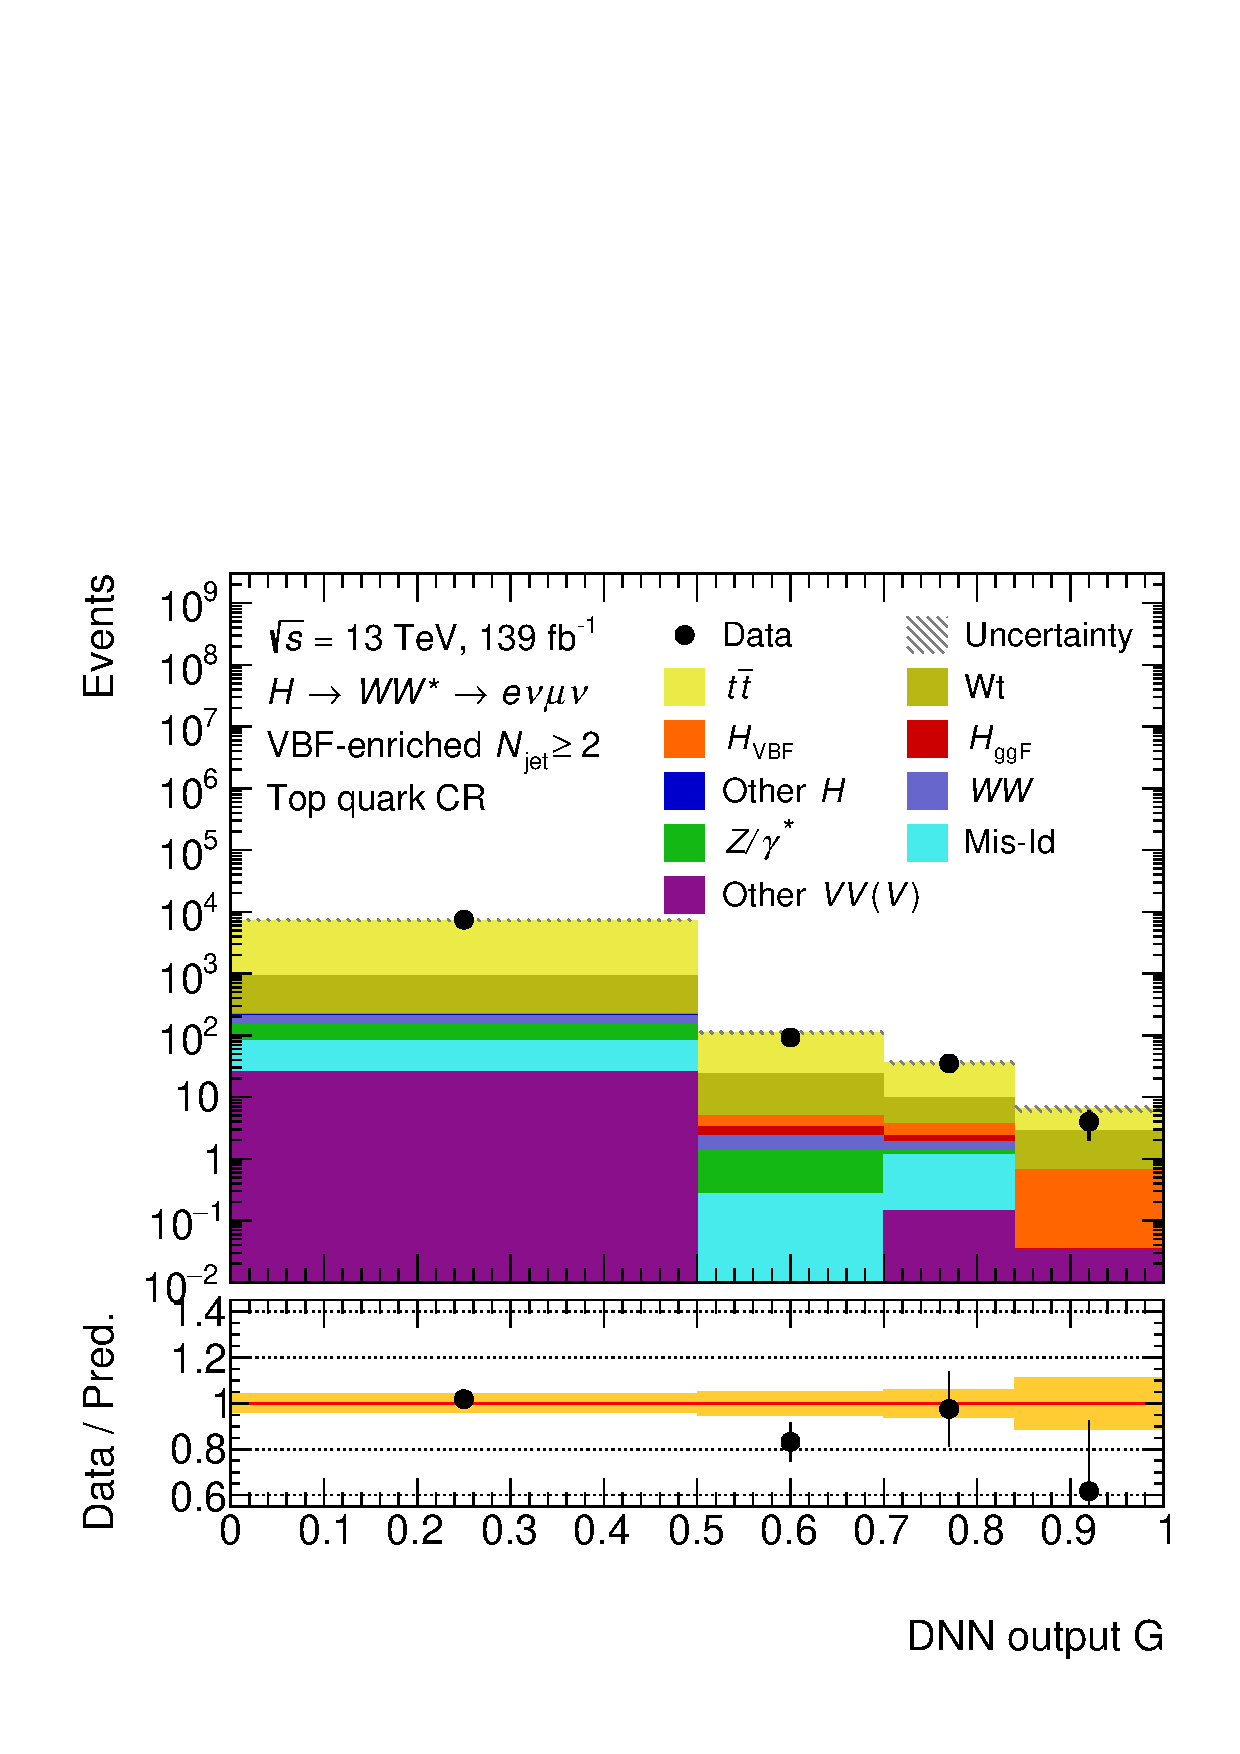
\includegraphics[width=0.32\textwidth]{figures/220605-Thesis/topcr/stxs/plots/run2-emme-CutVBF_TopControl_2jet_MJJ_350_700_PTH_0_200-DNNoutputG_FitBin1-log.pdf} \hfill
    }
    \subfloat[{\tiny $\mjj \geq 700~\GeV, \pTH < 200~\GeV$}]{
        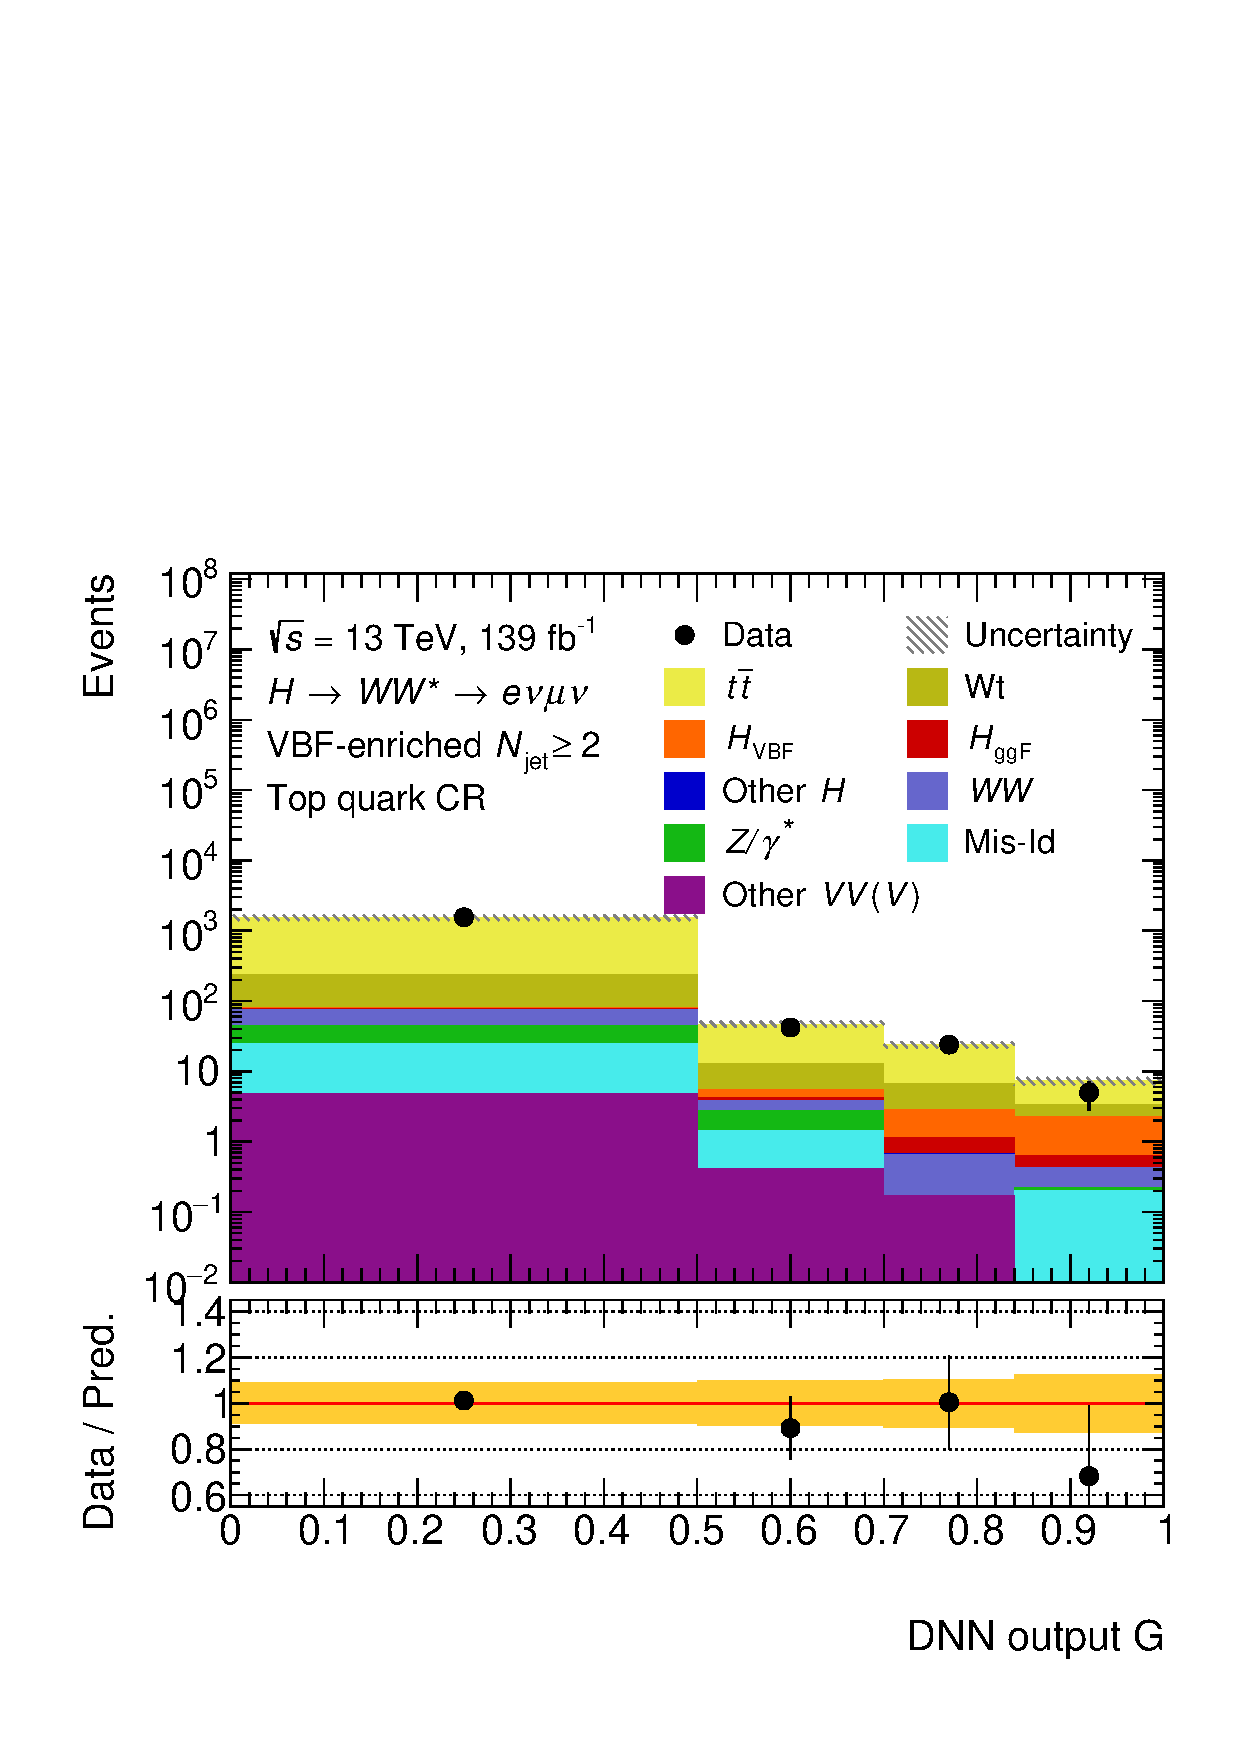
\includegraphics[width=0.32\textwidth]{figures/220605-Thesis/topcr/stxs/plots/run2-emme-CutVBF_TopControl_2jet_MJJ_GT700_PTH_0_200-DNNoutputG_FitBin1-log.pdf} \hfill
    }
    \subfloat[{\tiny $\mjj \geq 350~\GeV, \pTH \geq 200~\GeV$}]{
        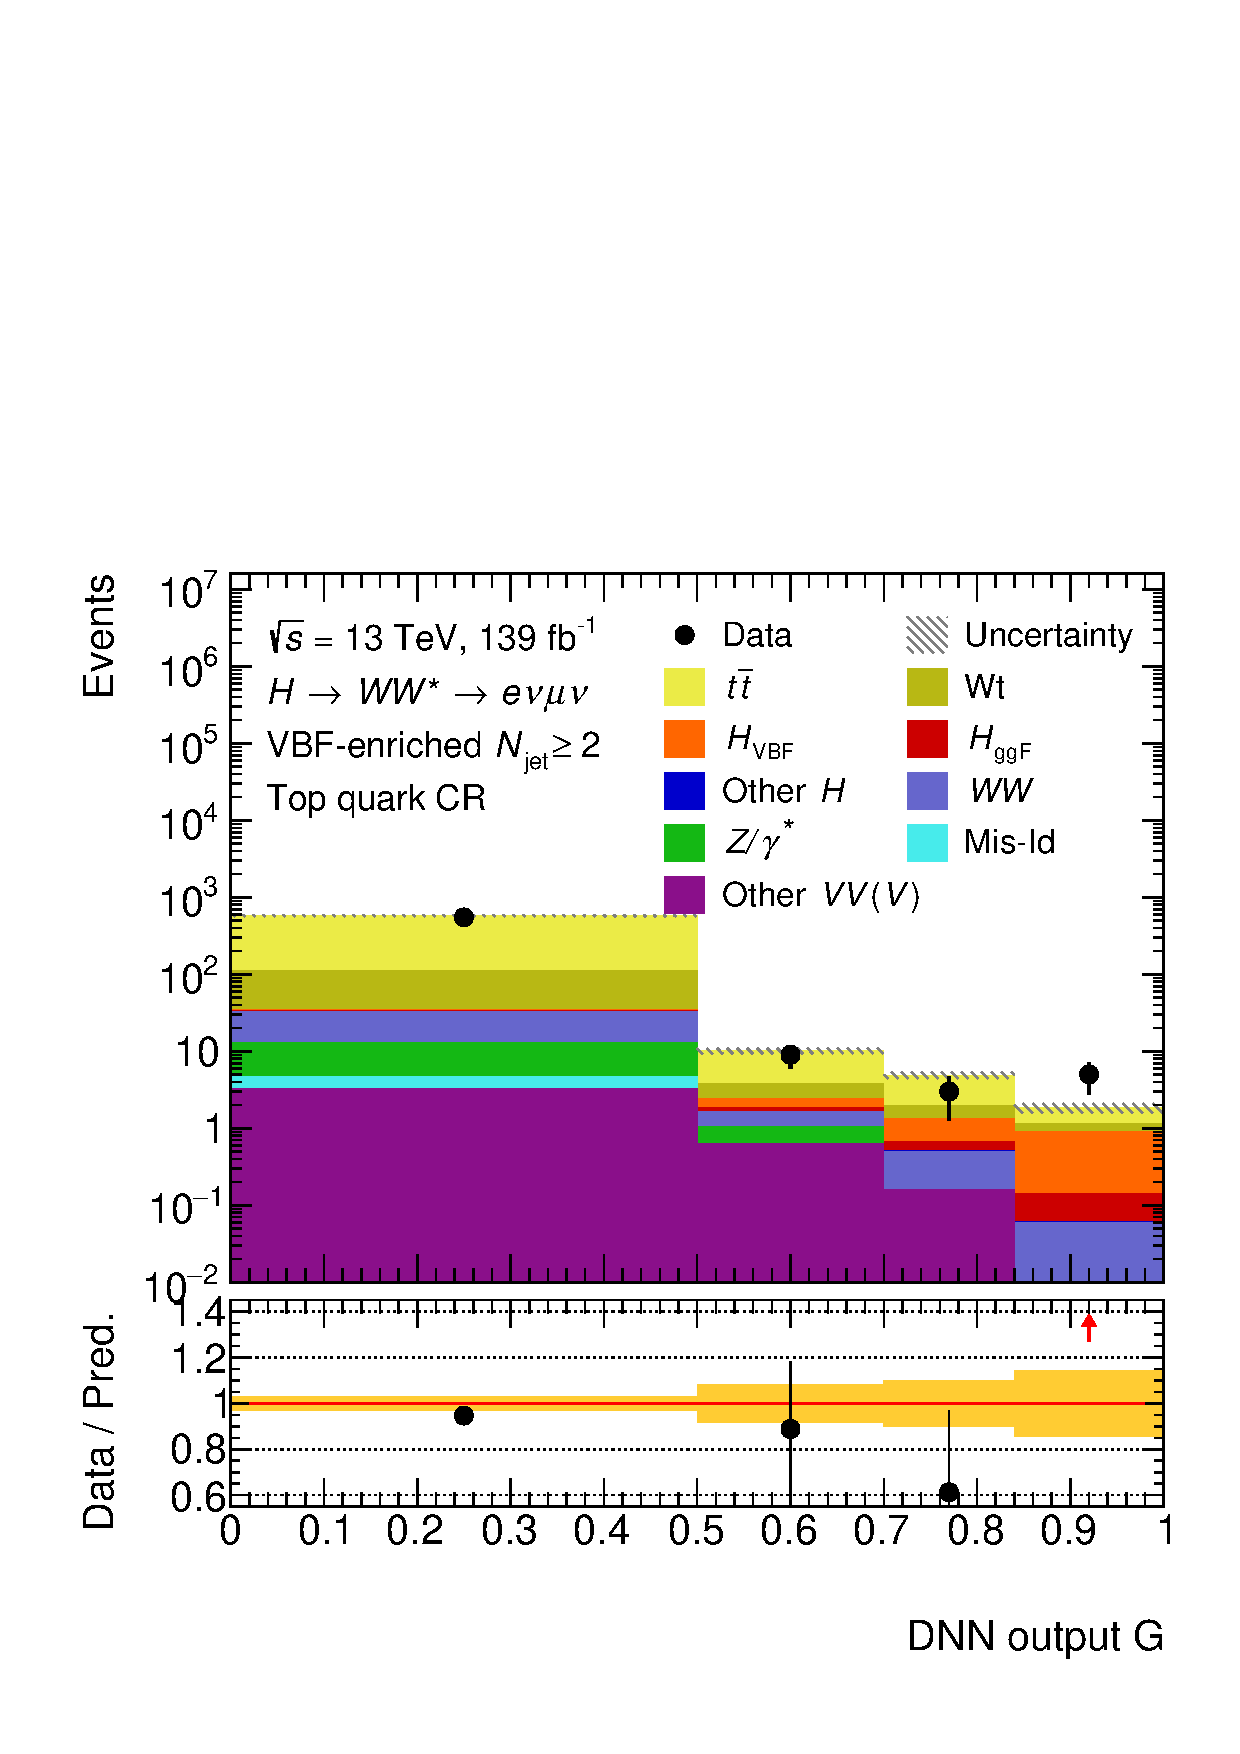
\includegraphics[width=0.32\textwidth]{figures/220605-Thesis/topcr/stxs/plots/run2-emme-CutVBF_TopControl_2jet_MJJ_GT350_PTH_GT200-DNNoutputG_FitBin1-log.pdf} \hfill
    }  \\
    \subfloat[{\tiny $350 \leq \mjj < 700~\GeV, \pTH < 200~\GeV$}]{
        \includegraphics[width=0.32\textwidth]{figures/220605-Thesis/zttcr/stxs/plots/run2-emme-CutVBF_ZtautauControl_2jet_MJJ_350_700_PTH_0_200-DNNoutputG_FitBin1-log.pdf} \hfill
    }
    \subfloat[{\tiny $\mjj \geq 700~\GeV, \pTH < 200~\GeV$}]{
        \includegraphics[width=0.32\textwidth]{figures/220605-Thesis/zttcr/stxs/plots/run2-emme-CutVBF_ZtautauControl_2jet_MJJ_GT700_PTH_0_200-DNNoutputG_FitBin1-log.pdf} \hfill
    }
    \subfloat[{\tiny $\mjj \geq 350~\GeV, \pTH \geq 200~\GeV$}]{
        \includegraphics[width=0.32\textwidth]{figures/220605-Thesis/zttcr/stxs/plots/run2-emme-CutVBF_ZtautauControl_2jet_MJJ_GT350_PTH_GT200-DNNoutputG_FitBin1-log.pdf} \hfill
    }
    {\caption{Distribution of the DNN output in the (a)-(c) top-quark CRs and (d)-(f) \Ztautau CRs used in the VBF, STXS analysis.
            \label{fig:dnn-output-vbf-stx} }}
\end{figure}
\captionsetup[subfloat]{captionskip=7pt} % space between subfloat caption and image


\FloatBarrier
\section{Event Selections in the ggF \ZeroJet and \OneJet Category}

\begin{figure}[!h]
    \centering
    \subfloat[]{
      \includegraphics[width=0.49\textwidth]{\paperfiguredir/ggF/ZeroJet/CutGGF_Ptll_0jet-Mll}
    }
    \subfloat[]{
      \includegraphics[width=0.49\textwidth]{\paperfiguredir/ggF/ZeroJet/CutGGF_bVeto_0jet-DPhill}
    } \\
    \subfloat[]{
      \includegraphics[width=0.49\textwidth]{\paperfiguredir/ggF/OneJet/CutGGF_ZttVeto_1jet-Mll}
    }
    \subfloat[]{
      \includegraphics[width=0.49\textwidth]{\paperfiguredir/ggF/OneJet/CutGGF_TopoMll_1jet-DPhill}
    }
  \caption{
  Distributions of (a) \mll and (b) \dphill in the \ZeroJet category as well as (c) \mll and (d) \dphill in the \OneJet category, after the preselection and background rejection steps, and also after the selection on \mll for the \dphill plots. The dashed lines indicate where the selection on the observable is made. The distributions are normalized to
  their nominal yields, before the final fit to all SRs and CRs (pre-fit normalizations). The hatched band shows the normalization component of the total pre-fit uncertainty, assuming SM Higgs boson production. The bottom panels show the normalized distributions for the signal and backgrounds, from which it can be inferred which background processes are primarily removed by the indicated selections.
  Figure and caption taken from \cref{HWWPaper}. 
  \label{fig:ggf:Plots:selections}
  }
  \end{figure}
  

\FloatBarrier
\section{STXS Measurement}
\label{app:stxs-measurement}
\begin{table}[htp]
    \caption{
    Best-fit values and uncertainties for the production cross section times $\hww$ branching fraction $({\sigma_i \cdot \mathcal{B}_{H \to WW^{\ast}}})$ in each STXS bin.
    }
    \begin{center}
      \small
      \renewcommand{\arraystretch}{1.5}
      \scalebox{0.90}{
        \begin{tabular}{l|rccccc|S[table-format=5,table-number-alignment=right]@{$\,\pm\,$}
  S[table-format=3,table-number-alignment=left]}
\toprule
\multirow{2}{*}{STXS bin $({\sigma_i \cdot \mathcal{B}_{H \to WW^{\ast}}})$} & \multicolumn{1}{c}{Value} & \multicolumn{5}{c|}{ Uncertainty [fb]} & \multicolumn{2}{c}{SM prediction} \\
&  \multicolumn{1}{c}{[fb]} &     Total                 & Stat.                       & Exp.\ Syst.                  & Sig.\ Theo.                  &    Bkg.\ Theo.    & \multicolumn{2}{c}{[fb]}   \\
\midrule
\makecell[l]{\noalign{\vskip 2mm} \ggHZeroJ  \\ {\scriptsize \ggHZeroJMath}}                  & $7100$                    & $^{+ 950}_{-910}$           & $^{+480}_{-470}$          & $^{+570}_{-530}$            & $^{+320}_{-260}$            & $^{+490}_{-480}$          & 5870  & 390           \\ [0.4cm]
\makecell[l]{\noalign{\vskip 1mm}\ggHOneJVLowPt  \\ {\scriptsize \ggHOneJVLowPtMath}}          & $1140$                    & $^{+ 800}_{-820}$           & $^{+420}_{-410}$          & $^{+380}_{-380}$            & $^{+80\phantom{0}}_{-70}$   & $^{+570}_{-600}$          & 1400 &  190            \\ [0.4cm]
\makecell[l]{\ggHOneJLowPt  \\ {\scriptsize \ggHOneJLowPtMath}}                 & $540$                     & $^{+ 470}_{-470}$           & $^{+310}_{-310}$          & $^{+230}_{-230}$            & $^{+42\phantom{0}}_{-47}$   & $^{+270}_{-280}$          & 970  & 150             \\ [0.4cm]
\makecell[l]{\ggHOneJMedPt  \\ {\scriptsize \ggHOneJMedPtMath}}                 & $230$                     & $^{+ 130}_{-120}$           & $^{+100}_{-100}$ & $^{+60\phantom{0}}_{-60}$   & $^{+10\phantom{0}}_{-10}$   & $^{+50\phantom{0}}_{-50}$ & 160  & 30             \\ [0.4cm]
\makecell[l]{\ggHTwoJ  \\ {\scriptsize \ggHTwoJMath}}                     & $1610$                    & $^{+ 900}_{-890}$           & $^{+440}_{-440}$          & $^{+430}_{-420}$            & $^{+300}_{-150}$   & $^{+640}_{-650}$          & 1010  & 220             \\ [0.4cm]
\makecell[l]{\ggHHighPt  \\ {\scriptsize \ggHHighPtMath}}                  & $260$                     & $^{+ 100}_{-100}$           & $^{+80\phantom{0}}_{-80}$ & $^{+40\phantom{0}}_{-40}$   & $^{+40\phantom{0}}_{-20}$   & $^{+40\phantom{0}}_{-40}$ & 122 & 31             \\ [0.4cm]
\makecell[l]{\qqHLowMjj \\ {\scriptsize \qqHLowMjjMath}}                  & $6$                     & $^{+ 63\phantom{0}}_{-62}$  & $^{+46\phantom{0}}_{-42}$ & $^{+31\phantom{0}}_{-34}$   & $^{+11\phantom{0}}_{-14}$   & $^{+24\phantom{0}}_{-26}$ & 109 & 7             \\ [0.4cm]
\makecell[l]{\qqHMedMjj \\ {\scriptsize \qqHMedMjjMath}}                   & $31$                      & $^{+ 35\phantom{0}}_{-33}$  & $^{+30\phantom{0}}_{-27}$ & $^{+15\phantom{0}}_{-14}$   & $^{+8\phantom{0}}_{-7}$    & $^{+11\phantom{0}}_{-10}$ & 56 & 4             \\ [0.4cm]
\makecell[l]{\qqHHighMjj \\ {\scriptsize \qqHHighMjjMath}}                 & $60$                      & $^{+ 26\phantom{0}}_{-23}$  & $^{+23\phantom{0}}_{-21}$ & $^{+7\phantom{00}}_{-7}$    & $^{+9\phantom{00}}_{-5}$    & $^{+5\phantom{00}}_{-5}$  & 51 & 4            \\ [0.4cm]
\makecell[l]{\qqHVHighMjj \\ {\scriptsize \qqHVHighMjjMath}}          & $57$                      & $^{+ 20\phantom{0}}_{-18}$  & $^{+18\phantom{0}}_{-17}$ & $^{+5\phantom{00}}_{-5}$    & $^{+3\phantom{00}}_{-3}$    & $^{+4\phantom{00}}_{-4}$  & 50 & 4             \\ [0.4cm]
\makecell[l]{\qqHHighPt \\ {\scriptsize   \qqHHighPtMath}}                & $37$                      & $^{+ 16\phantom{0}}_{-14}$  & $^{+14\phantom{0}}_{-13}$ & $^{+4\phantom{00}}_{-3}$    & $^{+4\phantom{00}}_{-3}$    & $^{+3\phantom{00}}_{-3}$  & 32 & 1            \\ [0.4cm]
\bottomrule
\end{tabular}

      }
    \end{center}
    \label{tab:STXS-XSecs}
  \end{table}

\FloatBarrier
\section{STXS Stage-1.2 Framework}
\label{app:stxs-measurements-aux}

\Cref{fig:stxs:stage-12-definition} shows the definitions of the fiducial kinematic regions in the Stage-1.2 STXS framework, including an indication of the merged regions measured in the \HWW analysis. 

\begin{figure}[h]
    \centering
    \subfloat[]{
        \newImageResizeCustom{0.9}{figures/hww/stxs/ggFSTXS-measured.pdf}
    } \\
    \subfloat[]{
        \newImageResizeCustom{0.9}{figures/hww/stxs/VBFSTXS-measured.pdf}
    } \\
    {\caption{Definition of fiducial kinematic regions in the Stage-1.2 STXS framework for (a) $ggH$ and (b) EW $qqH$ production. The colored boxes indicate the merged regions measured in the \HWW analysis.
            \label{fig:stxs:stage-12-definition} }}
\end{figure}


\chapter{Improvements of the \TwoJet Categories using Multiclass Classification}
\label{app:multi-class-2jet-strategy}

% %-----------------------------------------------------------------------
% %-----------------------------------------------------------------------
% \chapter{Mismodelling of data at the jet constituent level}
% \label{app:constituents-mismodelling}

% The reason is the challenge to model pile-up correctly, as it is impacted by non-perturbative effects.

% The MC samples therefore rely on theoretical models which parameters are \emph{tuned} to correctly describe the data in as many variables as possible.

% The effect is constant with pile-up and independent of the energy of the jet. The jet calibration can thereforegreatly reduce the effects of this mismodelling.

% \TDinote{Checkout notes for pile-up task force meetings}

% %-----------------------------------------------------------------------
% %-----------------------------------------------------------------------
% \chapter{Noise Term Measurement for \Rscan Jets}
% \label{app:noise-term-rscan}


% \section{Cluster Weighting}
% An alternative approach to correct for energy losses is the so-called \emph{local hadronic cell weighting} (LCW), which applies energy corrections already at cluster level.
% This approach is used for different jet definitions, one of which is described in \cref{app:noise-term-rscan}
% Different variables can be defined to characterize a topo-cluster based on its shape and other properties. These observables, known as \emph{cluster moments}, are used to extract information about the hadronic signal content in a given cluster which in turn is used to correct the energy to the \emph{LCW scale}. More information can be found in \ccite{PERF-2014-07}.

% \section{Definition and Calibration of \Rscan jets}

% \section{Changes to Noise Term Measurement}

% - Additional uncertainty from mu=0 fit range

% - Additional uncertainty based on the difference between different parametrisations


% \section{Results}
